\batchmode
\documentclass[a4paper]{book}
\usepackage{makeidx}
\usepackage{graphicx}
\usepackage{multicol}
\usepackage{float}
\usepackage{listings}
\usepackage{color}
\usepackage{ifthen}
\usepackage[table]{xcolor}
\usepackage{textcomp}
\usepackage{alltt}
\usepackage[utf8]{inputenc}
\usepackage{mathptmx}
\usepackage[scaled=.90]{helvet}
\usepackage{courier}
\usepackage{doxygen}
\lstset{language=C++,inputencoding=utf8,basicstyle=\footnotesize,breaklines=true,breakatwhitespace=true,tabsize=4,numbers=left }
\makeindex
\setcounter{tocdepth}{3}
\renewcommand{\footrulewidth}{0.4pt}
\begin{document}
\begin{titlepage}
\vspace*{7cm}
\begin{center}
{\Large FTGL \\[1ex]\large 2.1.3$\sim$rc5 }\\
\vspace*{1cm}
{\large Generated by Doxygen 1.7.2}\\
\vspace*{0.5cm}
{\small Tue Apr 8 2014 13:53:05}\\
\end{center}
\end{titlepage}
\clearemptydoublepage
\pagenumbering{roman}
\tableofcontents
\clearemptydoublepage
\pagenumbering{arabic}
\chapter{FTGL User Guide}
\label{index} 
\begin{DoxyImageNoCaption}
  \mbox{
\includegraphics[width=0.3\textwidth]{logo.png}}
\end{DoxyImageNoCaption}
\section{Introduction}\label{index_intro}
OpenGL doesn't provide direct font support, so the application must use any of OpenGL's other features for font rendering, such as drawing bitmaps or pixmaps, creating texture maps containing an entire character set, drawing character outlines, or creating a 3D geometry for each character.

More information can be found on the OpenGL website:
\begin{DoxyItemize}
\item {\tt http://www.opengl.org/resources/faq/technical/fonts.htm}
\item {\tt http://www.opengl.org/resources/features/fontsurvey/}
\end{DoxyItemize}

Most of these systems require a pre-\/processing stage to take the native fonts and convert them into a proprietary format.

FTGL was born out of the need to treat fonts in OpenGL applications just like any other application. For example when using Adobe Photoshop or Microsoft Word you don't need an intermediate pre-\/processing step to use high quality scalable fonts.\section{Documentation}\label{index_documentation}

\begin{DoxyItemize}
\item \doxyref{FTGL tutorial}{p.}{ftgl-tutorial}
\end{DoxyItemize}


\begin{DoxyItemize}
\item C API reference:
\begin{DoxyItemize}
\item \doxyref{FTGlyph.h}{p.}{FTGlyph_8h}
\item \doxyref{FTFont.h}{p.}{FTFont_8h}
\item \doxyref{FTLayout.h}{p.}{FTLayout_8h}
\end{DoxyItemize}
\end{DoxyItemize}


\begin{DoxyItemize}
\item C++ API reference:
\begin{DoxyItemize}
\item class \doxyref{FTGlyph}{p.}{classFTGlyph}
\item class \doxyref{FTFont}{p.}{classFTFont}
\item class \doxyref{FTLayout}{p.}{classFTLayout}
\end{DoxyItemize}
\end{DoxyItemize}\section{Additional information}\label{index_information}

\begin{DoxyItemize}
\item \doxyref{Frequently Asked Questions}{p.}{ftgl-faq}
\end{DoxyItemize}


\begin{DoxyItemize}
\item \doxyref{Projects using FTGL}{p.}{ftgl-projects} 
\end{DoxyItemize}
\chapter{Frequently Asked Questions}
\label{ftgl-faq}
\section{FAQ}\label{ftgl-faq_faq}
\subsection{When I try to compile \%FTGL it complains about a missing file from the include: \#include $<$ft2build.h$>$}\label{ftgl-faq_faq1}
FTGL relies on FreeType 2 for opening and decoding font files. This include is the main include for FreeType. You will need to download Freetype 2 and install it. Then make sure that the FTGL project that you are using points to your FreeType installation.\subsection{Is it possible to map a font to a \char`\"{}unit\char`\"{} size? My application relies on the fonts being a certain \char`\"{}physical\char`\"{} height (in OpenGL coordinate space) rather than a point size in display space. Any thoughts/suggestions?}\label{ftgl-faq_faq2}
We can do anything:) It would be easy to allow you to set the size in pixels, though I'm not sure this is what you want. Setting the size to 'OpenGL units' may be a bit harder. What does 1.0 in opengl space mean and how does that relate to point size? For one person it might mean scaling the font up, for someone else it may mean scaling down. Plus bitmaps and pixmaps have a pixel to pixel relationship that you can't change.

Here's some guidelines for vector and texture fonts. Take note that I say 'should' a lot :)


\begin{DoxyItemize}
\item One point in pixel space maps to 1 unit in OpenGL space, so a glyph that is 18 points high should be 18.0 units high.
\end{DoxyItemize}


\begin{DoxyItemize}
\item If you set an ortho projection to the window size and draw a glyph it's screen size should be the correct physical size ie a 72 point glyph on a 72dpi screen will be 1 inch high. Also if you set a perspective projection that maps 0.0 in the z axis to screen size you will get the same eg. 
\begin{DoxyCode}
gluPerspective(90, window_height / 2 , small_number, large_number);
\end{DoxyCode}
 So basically it all depends on your projection matrix. Obviously you can use glScale but I understand if you don't want to.
\end{DoxyItemize}

Couple of extra things to note:


\begin{DoxyItemize}
\item The quality of vector glyphs will not change when you change the size, ie. a really small polygon glyph up close will look exactly the same as a big one from far away. They both contain the same amount of data. This doesn't apply to texture fonts.
\end{DoxyItemize}


\begin{DoxyItemize}
\item Secondly, there is a bug in the advance/kerning code that will cause ugliness at really small point sizes. This is because the advance and kerning use ints so an advance of 0.4 will become zero. If this is going to be a probelm, I can fix this.
\end{DoxyItemize}

Early on I did a lot of head scratching over the OpenGL unit to font size thing because when I was first integrating FTGL into my engine the fonts weren't the size I was expecting. I was tempted to build in some scaling but I decided doing nothing was the best approach because you can't please everyone. Plus it's 'correct' as it is. 
\chapter{Projects using FTGL}
\label{ftgl-projects}
To add your project to this list, please contact one of the FTGL developers at {\tt http://sf.net/projects/ftgl}

Projects are listed in alphabetical order.\section{\%FTGL language bindings}\label{ftgl-projects_bindings}
\subsection{\%FTGL\#}\label{ftgl-projects_ftglsharp}
FTGL\# ({\tt http://www.paskaluk.com/projects.php}) is a collection of .NET bindings for FTGL.\subsection{GlGuiA}\label{ftgl-projects_glguia}
GlGuiA ({\tt http://sourceforge.net/projects/glguia/}) is a set of packages for Ada 2006 that can be used to create Graphical User Interfaces, relaying (almost) only on OpenGl. Hence should be rather platform-\/independant.\subsection{Ruby \%FTGL}\label{ftgl-projects_ruby-ftgl}
Ruby FTGL\# ({\tt http://rubyforge.org/projects/ruby-\/ftgl/}) is a collection of Ruby bindings for FTGL.\subsection{PyFTGL}\label{ftgl-projects_pyftgl}
PyFTGL ({\tt http://code.google.com/p/pyftgl/}) wraps the functionality of FTGL into a Python module so that it can be used in conjunction with PyOpenGL.\section{Projects currently using \%FTGL}\label{ftgl-projects_current}
\subsection{Agent World}\label{ftgl-projects_agentw}
Agent World ({\tt http://code.google.com/p/agentw/}) provides tools for simulating and visualizing multi-\/agent systems and is specially designed for testing machine learning applications (and specially focused on Case Based Reasoning ones). It includes support for representing information using the Feature Term formalism, and provides a series of relational machine learning algorithms that can deal with them. The whole project is created in C++ to maximize efficiency, and uses OpenGL as the visualization library to ensure cross-\/platformness.\subsection{Amaltheia}\label{ftgl-projects_amaltheia}
Amaltheia ({\tt http://home.gna.org/amaltheia/}) is a cross-\/platform game programming API that supports two backends, OpenGL and DirectX. The aim of the Amaltheia project is to create an intuitive and simple to use library, providing core 3d and 2d functionality in a platform independent manner. It also provides platform independence regarding basic network functions, input handling, threads and sound. Currently the GNU/Linux and the Windows OSes are supported.\subsection{Armagetron Advanced}\label{ftgl-projects_armagetronad}
Armagetron Advanced ({\tt http://www.armagetronad.net/}) is a multiplayer game in 3d that attempts to emulate and expand on the lightcycle sequence from the movie Tron. It's an old school arcade game slung into the 21st century. Highlights include a customizable playing arena, HUD, unique graphics, and AI bots. For the more advanced player there are new game modes and a wide variety of physics settings to tweak as well.\subsection{Audicle}\label{ftgl-projects_audicle}
Audicle ({\tt http://audicle.cs.princeton.edu/}) is an audio programming environment that integrates the programmability of the development environment with elements of the runtime environment. The result is a duct-\/taped intersection of a concurrent smart editor, compiler, virtual machine, and debugger.\subsection{Battlestar T.U.X.}\label{ftgl-projects_battlestartux}
Battlestar T.U.X. ({\tt http://code.google.com/p/battlestar-\/tux/}) is a top-\/down scrolling shooter project.\subsection{BJS}\label{ftgl-projects_bjs}
BJS ({\tt http://bjs.sourceforge.net/}) is a funny arcade 3D multiplayer tank battle. It is fuly playable and very fun in multiplayer. Of course the single player is also possible. There is no story. You just get a tank and go shoot other players. Currently there are 5 different tanks, 6 maps, 9 powerups and 4 weapons.\subsection{Blender}\label{ftgl-projects_blender}
Blender ({\tt http://blender.org/}) is an integrated 3d suite for modelling, animation, rendering, post-\/production, interactive creation and playback (games).\subsection{Breve}\label{ftgl-projects_breve}
Breve ({\tt http://www.spiderland.org/}) is a free, open-\/source software package which makes it easy to build 3D simulations of multi-\/agent systems and artificial life. Using Python, or using a simple scripting language called steve, you can define the behaviors of agents in a 3D world and observe how they interact. breve includes physical simulation and collision detection so you can simulate realistic creatures, and an OpenGL display engine so you can visualize your simulated worlds.\subsection{BZFlag}\label{ftgl-projects_bzflag}
BZFlag ({\tt http://BZFlag.org/}) is a 3D multi-\/player multiplatform tank battle game that allows users to play against each other in a network environment.

BZFlag uses FTGL as of version 2.99.\subsection{Capture The Flag}\label{ftgl-projects_capturetf}
Capture The Flag ({\tt http://capturetf.sourceforge.net/}) is an open source, multi-\/platform, network game project.\subsection{Cello}\label{ftgl-projects_cello}
Cello ({\tt http://common-\/lisp.net/project/cello/}) is a project to create an open-\/source, industrial-\/strength, portable GUI toolkit for Common Lisp. Its features include anti-\/aliased fonts, accelerated 2d-\/ and 3d-\/graphics, a standard set of GUI widgets, easy construction of new widgets, and much more. Cello heavily utilizes Cells (a sister project on common-\/lisp.net), in addition to industry-\/standard technologies such as OpenGL, FreeType, and ImageMagick.\subsection{Chimera}\label{ftgl-projects_chimera}
Chimera ({\tt http://www.cgl.ucsf.edu/chimera/}) is a highly extensible program for interactive visualization and analysis of molecular structures and related data, including density maps, supramolecular assemblies, sequence alignments, docking results, trajectories, and conformational ensembles. High-\/quality images and animations can be generated.\subsection{Cinepaint}\label{ftgl-projects_cinepaint}
Cinepaint ({\tt http://www.cinepaint.org/}) is a deep paint image retouching tool that supports higher color fidelity than ordinary painting tools.\subsection{Duel}\label{ftgl-projects_duel}
Duel ({\tt http://www.personal.rdg.ac.uk/$\sim$sir03me/play/code.html}) is a small overhead perspective spaceship game.\subsection{Empty Clip}\label{ftgl-projects_emptyclip}
Empty Clip ({\tt http://emptyclip.sourceforge.net/}) is a top-\/down 2D Action RPG.\subsection{Freebox}\label{ftgl-projects_freebox}
Freebox ({\tt http://freebox.sourceforge.net/}) is designed for use in a special type of computer called an 'HTPC', which is connected to a home-\/theatre system to watch XviD/DivX/DVD movies, play music (MP3, CD, whatever), play some emulated games, or whatever else you want to do with it.\subsection{Gem}\label{ftgl-projects_gem}
Gem ({\tt http://gem.iem.at/}) is a loadable library for puredata, which adds OpenGL graphics rendering and animation to Pd. Pd is a graphical programming language and computer music system.\subsection{GLMayan}\label{ftgl-projects_glmayab}
GLMayan ({\tt http://glmayan.sourceforge.net/}) is an OpenGL screensaver.\subsection{Glover}\label{ftgl-projects_glover}
Glover ({\tt http://code.google.com/p/glover/}) is a movie player that renders the content using openGL allowing all kinds of special effects using fragment shaders. The movie decoding is done using ffmpeg.\subsection{Ivf++}\label{ftgl-projects_ivfplusplus}
Ivf++ ({\tt http://ivfplusplus.sourceforge.net/}) is a C++ library encapsulating OpenGL functionality. The primary goal is to make it easier to use the OpenGL library in interactive 3D applications. The second goal is extendibility, providing a set of well defined base classes for different object types to build new classes on. The third goal is portability, primarily between Linux and Windows, but the library should also be easily ported to Mac OS X.\subsection{Jahshaka}\label{ftgl-projects_jahshaka}
Jashaka ({\tt http://jahshaka.org/}) is an advanced video editing, animation, visual effects, painting and music tool.\subsection{Karaoke FX}\label{ftgl-projects_karaokefx}
Karaoke FX ({\tt http://jeanchristophe.duber.free.fr/karaokefx/}) is a midifile player that can display lyrics in synch whith the sound so as it can be used for karaoke. It relies on plugins for midi output devices as for lyrics display.\subsection{Libinstrudeo}\label{ftgl-projects_libinstrudeo}
Libinstrudeo ({\tt http://sourceforge.net/projects/libinstrudeo}), initially written for the ScreenKast program, provides the necessary logic to capture screen recordings and to process them. Includes a soap-\/client for the webservice at captorials.com that enables you to share your recordings.\subsection{Light Speed!}\label{ftgl-projects_lightspeed}
Light Speed! ({\tt http://lightspeed.sourceforge.net/}) is an OpenGL-\/based program which illustrates the effects of special relativity on the appearance of moving objects. When an object accelerates past a few million meters per second, these effects begin to grow noticeable, becoming more and more pronounced as the speed of light is approached. These relativistic effects are viewpoint-\/dependent, and include shifts in length, object hue, brightness and shape.\subsection{MySQL GUI Tools}\label{ftgl-projects_mysqlguitools}
MySQL GUI Tools ({\tt http://dev.mysql.com/downloads/gui-\/tools/5.0.html}) is a collection of tools for the MySQL database. It consists of MySQL Administrator, MySQL Query Browser and MySQL Migration Toolkit.\subsection{OctPlot}\label{ftgl-projects_octplot}
OctPlot ({\tt http://octplot.sourceforge.net/}) is a graphics package for Octave, the free alternative to MATLAB. It provides high quality PostScript and on-\/screen graphics.\subsection{Open ActiveWrl}\label{ftgl-projects_openactivewrl}
Open ActiveWrl ({\tt http://open-\/activewrl.sourceforge.net/}) is a software development toolkit based on a generic software development approach that allows the implementation VRML/X3D browser componentes. These browser components can run within an conventional application or can be linked together for the implementation of parallel immersive VR setups.\subsection{OpenEaagles}\label{ftgl-projects_openeaagles}
OpenEaagles ({\tt http://www.openeaagles.org/}) is a multi-\/platform simulation framework targeted to help simulation engineers and software developers build robust, scalable, virtual, constructive, stand-\/alone, and distributed simulation applications. It has been used extensively to build applications that demand real-\/time performance. This includes applications to conduct human factor studies, operator training, and the development of complete distributed virtual simulation systems. OpenEaagles has also been used to build stand-\/alone and distributed constructive applications oriented at system analysis.\subsection{OpenGC}\label{ftgl-projects_opengc}
OpenGC ({\tt http://www.opengc.org/}) is a multi-\/platform, multi-\/simulator, open-\/source C++ tool for developing and implementing high quality glass cockpit displays for simulated flightdecks.\subsection{OpenSG}\label{ftgl-projects_opensg}
OpenSG ({\tt http://www.opensg.org/}) is a portable scenegraph system to create realtime graphics programs, e.g. for virtual reality applications.\subsection{Panthera}\label{ftgl-projects_panthera}
Panthera ({\tt http://sourceforge.net/projects/panthera}) is a C++ framework for interactive visualization, manipulation, and editing of volume data. Applications developed on top of Panthera can utilize both desktop and immersive user interface devices, such as position trackers and haptic displays.\subsection{Planet Penguin Racer}\label{ftgl-projects_ppracer}
PlanetPenguin Racer ({\tt http://developer.berlios.de/projects/ppracer/}) is a simple OpenGL racing game featuring Tux, the Linux mascot. The goal of the game is to slide down a snow-\/ and ice-\/covered mountain as quickly as possible, avoiding the trees and rocks that will slow you down.\subsection{projectM}\label{ftgl-projects_projectm}
projectM ({\tt http://projectm.sourceforge.net/}) is a music visualizer which uses OpenGL for hardware acceleration. It is compatible with Milkdrop presets.\subsection{Puzzle Bobble 3D}\label{ftgl-projects_puzzle}
Puzzle Bobble 3D ({\tt http://homepage.mac.com/eric.lee/puzzle/}) is a 3D video game for Linux. The game is similar to Tetris/Connect 4: connect balls of the same colour to make them disappear. Puzzle Bobble 3D is based on an already popular arcade game of the same name by Taito Corporation (see links section at the bottom of this page), but this particular variant is played in a 3D environment (hence the name).\subsection{ROOT}\label{ftgl-projects_root}
ROOT ({\tt http://root.cern.ch/}) is an object-\/oriented data analysis framework.\subsection{SCIRun}\label{ftgl-projects_scirun}
SCIRun ({\tt http://software.sci.utah.edu/scirun.html}) is a Problem Solving Environment (PSE), for modeling, simulation and visualization of scientific problems. It is available for free and open source.\subsection{TINE}\label{ftgl-projects_tine}
TINE, or TINE Is Not ELITE ({\tt http://tine.sunsite.dk/en/index.html}) is an open source cross-\/platform remake of the classic space adventure game ELITE.\subsection{Tiny Planet}\label{ftgl-projects_tinyplanet}
Tiny Planet ({\tt http://www.duberga.net/tinyplanet/}) is a real-\/time OpenGL viewer of detailled earth texture such as BlueMarble from Earth Observatory (NASA) or any other planet texture. Vectorial data such as points of interest, boundaries, rivers can be superimposed to the texture.\subsection{Truevision}\label{ftgl-projects_truevision}
Truevision ({\tt http://truevision.sourceforge.net/}) is a 3D modeler for GNOME.\subsection{Tulip}\label{ftgl-projects_tulip}
Tulip ({\tt http://tulip.labri.fr/}) is a system dedicated to the visualization of huge graphs. It is capable of managing graphs with up to 500,000 nodes and edges on relatively modest hardware (eg. 600MHz Pentium III, 256MB RAM).\subsection{Ubit}\label{ftgl-projects_ubit}
Ubit ({\tt http://www.infres.enst.fr/$\sim$elc/ubit/}) Ubit is a new GUI toolkit that combines the advantages of scene graph and widget based toolkits. The Ubit3D extension makes it possible to display 2D GUIs in a 3D space.\subsection{VRS}\label{ftgl-projects_vrs}
The Virtual Rendering System ({\tt http://www.hpi.uni-\/potsdam.de/vrs/}) is a computer graphics software library for constructing interactive 3D applications. It provides a large collection of 3D rendering components which facilitate implementing 3D graphics applications and experimenting with 3D graphics and imaging algorithms.\subsection{VTK}\label{ftgl-projects_vtk}
VTK, the Visualization Toolkit ({\tt http://www.vtk.org/}), is an object oriented, high level library that allows one to easily write C++ programs, Tcl, Python and Java scripts that do 3D visualization.\subsection{XLock}\label{ftgl-projects_xlock}
XLock ({\tt http://www.tux.org/$\sim$bagleyd/xlockmore.html}) is a screensaver and screen locking utility with additional OpenGL and XPM modes.\section{Projects that used to use \%FTGL}\label{ftgl-projects_old}
\subsection{GNU Backgammon}\label{ftgl-projects_gnubg}
GNU Backgammon ({\tt http://www.gnubg.org/}) was using FTGL until version 0.14.3+20060520-\/1.\subsection{OpenSceneGraph}\label{ftgl-projects_openscenegraph}
OpenSceneGraph ({\tt http://www.openscenegraph.org/projects/osg}) is an open source high performance 3D graphics toolkit, used by application developers in fields such as visual simulation, games, virtual reality, scientific visualization and modelling. Written entirely in Standard C++ and OpenGL it runs on all Windows platforms, OSX, GNU/Linux, IRIX, Solaris, HP-\/Ux, AIX and FreeBSD operating systems.\subsection{Teddy}\label{ftgl-projects_teddy}
Teddy ({\tt http://teddy.sourceforge.net/}) was a 3D graphics library. The main purpose was to be a simple scene graph manager.\subsection{VigiPac}\label{ftgl-projects_vigipac}
VigiPac ({\tt http://vigipac.sourceforge.net/}) was a three-\/dimensional Pacman clone with multiplayer support, written in the C++ language. 
\chapter{FTGL tutorial}
\label{ftgl-tutorial}
\section{Starting to use \%FTGL}\label{ftgl-tutorial_starting}
Only one header is required to use FTGL:


\begin{DoxyCode}
#include <FTGL/ftgl.h>
\end{DoxyCode}
\section{Choosing a font type}\label{ftgl-tutorial_type}
FTGL supports 6 font output types among 3 groups: raster fonts, vector fonts, and texture fonts which are a mixture of both. Each font type has its advantages and disadvantages.\subsection{Raster fonts}\label{ftgl-tutorial_raster}
Raster fonts are made of pixels painted directly on the viewport's framebuffer. They cannot be directly rotated or scaled.


\begin{DoxyItemize}
\item Bitmap fonts use 1-\/bit (2-\/colour) rasterised glyphs.
\item Pixmap fonts use 8-\/bit (256 levels) rasterised glyphs.
\end{DoxyItemize}

 
\begin{DoxyImageNoCaption}
  \mbox{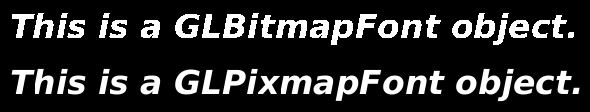
\includegraphics[width=0.7\textwidth]{rasterfont.png}}
\end{DoxyImageNoCaption}
\subsection{Vector fonts}\label{ftgl-tutorial_vector}
Vector fonts are 3D objects that are rendered at the current matrix location. All position, scale, texture and material effects apply to vector fonts.


\begin{DoxyItemize}
\item Polygon fonts use planar triangle meshes and can be texture-\/mapped.
\item Outline fonts use OpenGL lines.
\item Extruded fonts are extruded polygon fonts, with the front, back and side meshes renderable separately to apply different effects and materials.
\end{DoxyItemize}

 
\begin{DoxyImageNoCaption}
  \mbox{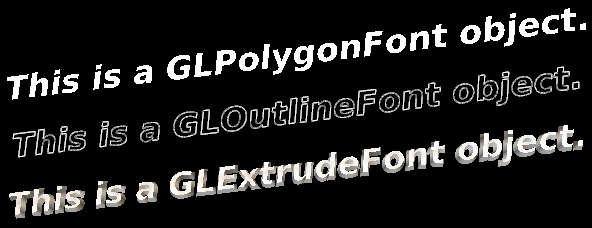
\includegraphics[width=0.7\textwidth]{vectorfont.png}}
\end{DoxyImageNoCaption}
\subsection{Textured fonts}\label{ftgl-tutorial_texture}
Textured fonts are probably the most versatile types. They are fast, antialiased, and can be transformed just like any OpenGL primitive.


\begin{DoxyItemize}
\item Texture fonts use one texture per glyph. They are fast because glyphs are stored permanently in the video card's memory.
\item Buffer fonts use one texture per line of text. They tend to be faster than texture fonts when the same line of text needs to be rendered for more than one frame.
\end{DoxyItemize}

 
\begin{DoxyImageNoCaption}
  \mbox{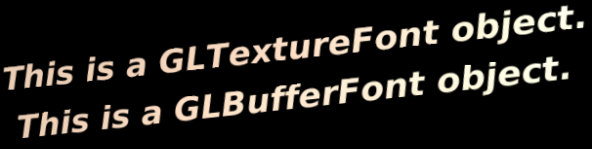
\includegraphics[width=0.7\textwidth]{texturefont.png}}
\end{DoxyImageNoCaption}
\section{Create font objects}\label{ftgl-tutorial_creating}
Creating a font and displaying some text is really straightforward, be it in C or in C++.\subsection{in C}\label{ftgl-tutorial_c}

\begin{DoxyCode}
/* Create a pixmap font from a TrueType file. */
FTGLfont *font = ftglCreatePixmapFont("/home/user/Arial.ttf");

/* If something went wrong, bail out. */
if(!font)
    return -1;

/* Set the font size and render a small text. */
ftglSetFontFaceSize(font, 72, 72);
ftglRenderFont(font, "Hello World!", FTGL_RENDER_ALL);

/* Destroy the font object. */
ftglDestroyFont(font);
\end{DoxyCode}
\subsection{in C++}\label{ftgl-tutorial_cxx}

\begin{DoxyCode}
// Create a pixmap font from a TrueType file.
FTGLPixmapFont font("/home/user/Arial.ttf");

// If something went wrong, bail out.
if(font.Error())
    return -1;

// Set the font size and render a small text.
font.FaceSize(72);
font.Render("Hello World!");
\end{DoxyCode}


The first 128 glyphs of the font (generally corresponding to the ASCII set) are preloaded. This means that usual text is rendered fast enough, but no memory is wasted loading glyphs that will not be used.\section{More font commands}\label{ftgl-tutorial_commands}
\subsection{Font metrics}\label{ftgl-tutorial_metrics}
 
\begin{DoxyImageNoCaption}
  \mbox{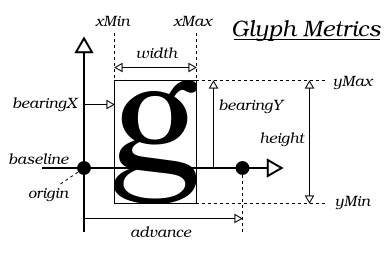
\includegraphics[width=0.5\textwidth]{metrics.png}}
\end{DoxyImageNoCaption}


If you ask a font to render at 0.0, 0.0 the bottom left most pixel or polygon may not be aligned to 0.0, 0.0. With \doxyref{FTFont::Ascender()}{p.}{classFTFont_ac4659028a0be30e8bc85814e7e53ee87}, \doxyref{FTFont::Descender()}{p.}{classFTFont_aa72f172f4f9a39970913e176f38866bc} and \doxyref{FTFont::Advance()}{p.}{classFTFont_ae606eb0323341d1a521dae7a712f1b6e} an approximate bounding box can be calculated.

For an exact bounding box, use the \doxyref{FTFont::BBox()}{p.}{classFTFont_a05b5c069ab8e958935096df78f8af16f} function. This function returns the extent of the volume containing 'string'. 0.0 on the y axis will be aligned with the font baseline.\subsection{Specifying a character map encoding}\label{ftgl-tutorial_charmap}
From the FreeType documentation:

"By default, when a new face object is created, (FreeType) lists all the charmaps contained in the font face and selects the one that supports Unicode character codes if it finds one. Otherwise, it tries to find support for Latin-\/1, then ASCII."

It then gives up. In this case FTGL will set the charmap to the first it finds in the fonts charmap list. You can expilcitly set the char encoding with \doxyref{FTFont::CharMap()}{p.}{classFTFont_a64f7346221e90325220829eeaa238e93}.

Valid encodings as of FreeType 2.0.4 are:


\begin{DoxyItemize}
\item ft\_\-encoding\_\-none
\item ft\_\-encoding\_\-unicode
\item ft\_\-encoding\_\-symbol
\item ft\_\-encoding\_\-latin\_\-1
\item ft\_\-encoding\_\-latin\_\-2
\item ft\_\-encoding\_\-sjis
\item ft\_\-encoding\_\-gb2312
\item ft\_\-encoding\_\-big5
\item ft\_\-encoding\_\-wansung
\item ft\_\-encoding\_\-johab
\item ft\_\-encoding\_\-adobe\_\-standard
\item ft\_\-encoding\_\-adobe\_\-expert
\item ft\_\-encoding\_\-adobe\_\-custom
\item ft\_\-encoding\_\-apple\_\-roman
\end{DoxyItemize}

For instance:


\begin{DoxyCode}
font.CharMap(ft_encoding_apple_roman);
\end{DoxyCode}


This will return an error if the requested encoding can't be found in the font.

If your application uses Latin-\/1 characters, you can preload this character set using the following code:


\begin{DoxyCode}
// Create a pixmap font from a TrueType file.
FTGLPixmapFont font("/home/user/Arial.ttf");

// If something went wrong, bail out.
if(font.Error())
    return -1;

// Set the face size and the character map. If something went wrong, bail out.
font.FaceSize(72);
if(!font.CharMap(ft_encoding_latin_1))
    return -1;

// Create a string containing all characters between 128 and 255
// and preload the Latin-1 chars without rendering them.
char buf[129];
for(int i = 128; i < 256; i++)
{
    buf[i] = (char)(unsigned char)i;
}
buf[128] = '\0';

font.Advance(buf);
}
\end{DoxyCode}
\section{Sample font manager class}\label{ftgl-tutorial_sample}

\begin{DoxyCode}
FTTextureFont* myFont = FTGLFontManager::Instance().GetFont("arial.ttf", 72);

#include <map>
#include <string>
#include <FTGL/ftgl.h>

using namespace std;

typedef map<string, FTFont*> FontList;
typedef FontList::const_iterator FontIter;

class FTGLFontManager
{
    public:
        // NOTE
        // This is shown here for brevity. The implementation should be in the so
      urce
        // file otherwise your compiler may inline the function resulting in
        // multiple instances of FTGLFontManager
        static FTGLFontManager& Instance()
        {
            static FTGLFontManager tm;
            return tm;
        }

        ~FTGLFontManager()
        {
            FontIter font;
            for(font = fonts.begin(); font != fonts.end(); font++)
            {
                delete (*font).second;
            }

            fonts.clear();
        }


        FTFont* GetFont(const char *filename, int size)
        {
            char buf[256];
            sprintf(buf, "%s%i", filename, size);
            string fontKey = string(buf);

            FontIter result = fonts.find(fontKey);
            if(result != fonts.end())
            {
                LOGMSG("Found font %s in list", filename);
                return result->second;
            }

            FTFont* font = new FTTextureFont;

            string fullname = path + string(filename);

            if(!font->Open(fullname.c_str()))
            {
                LOGERROR("Font %s failed to open", fullname.c_str());
                delete font;
                return NULL;
            }

            if(!font->FaceSize(size))
            {
                LOGERROR("Font %s failed to set size %i", filename, size);
                delete font;
                return NULL;
            }

            fonts[fontKey] = font;

            return font;
        }


    private:
        // Hide these 'cause this is a singleton.
        FTGLFontManager(){}
        FTGLFontManager(const FTGLFontManager&){};
        FTGLFontManager& operator = (const FTGLFontManager&){ return *this; };

        // container for fonts
        FontList fonts;
};
\end{DoxyCode}
 
\chapter{Namespace Documentation}
\section{FTGL Namespace Reference}
\label{namespaceFTGL}\index{FTGL@{FTGL}}
\subsection*{Enumerations}
\begin{DoxyCompactItemize}
\item 
enum {\bf RenderMode} \{ {\bf RENDER\_\-FRONT} =  0x0001, 
{\bf RENDER\_\-BACK} =  0x0002, 
{\bf RENDER\_\-SIDE} =  0x0004, 
{\bf RENDER\_\-ALL} =  0xffff
 \}
\item 
enum {\bf TextAlignment} \{ {\bf ALIGN\_\-LEFT} =  0, 
{\bf ALIGN\_\-CENTER} =  1, 
{\bf ALIGN\_\-RIGHT} =  2, 
{\bf ALIGN\_\-JUSTIFY} =  3
 \}
\end{DoxyCompactItemize}


\subsection{Enumeration Type Documentation}
\index{FTGL@{FTGL}!RenderMode@{RenderMode}}
\index{RenderMode@{RenderMode}!FTGL@{FTGL}}
\subsubsection[{RenderMode}]{\setlength{\rightskip}{0pt plus 5cm}enum {\bf FTGL::RenderMode}}\label{namespaceFTGL_a9916822cb1247bd2e1aae26f7bfec74e}
\begin{Desc}
\item[Enumerator: ]\par
\begin{description}
\index{RENDER\_\-FRONT@{RENDER\_\-FRONT}!FTGL@{FTGL}}\index{FTGL@{FTGL}!RENDER\_\-FRONT@{RENDER\_\-FRONT}}\item[{\em 
RENDER\_\-FRONT\label{namespaceFTGL_a9916822cb1247bd2e1aae26f7bfec74ea682a1ee1dff8218153646cfbe570bdae}
}]\index{RENDER\_\-BACK@{RENDER\_\-BACK}!FTGL@{FTGL}}\index{FTGL@{FTGL}!RENDER\_\-BACK@{RENDER\_\-BACK}}\item[{\em 
RENDER\_\-BACK\label{namespaceFTGL_a9916822cb1247bd2e1aae26f7bfec74ea13191d43484e1bfe32598e8cb894cef9}
}]\index{RENDER\_\-SIDE@{RENDER\_\-SIDE}!FTGL@{FTGL}}\index{FTGL@{FTGL}!RENDER\_\-SIDE@{RENDER\_\-SIDE}}\item[{\em 
RENDER\_\-SIDE\label{namespaceFTGL_a9916822cb1247bd2e1aae26f7bfec74ea5ce274c9f80d8a48fbe026329885cf92}
}]\index{RENDER\_\-ALL@{RENDER\_\-ALL}!FTGL@{FTGL}}\index{FTGL@{FTGL}!RENDER\_\-ALL@{RENDER\_\-ALL}}\item[{\em 
RENDER\_\-ALL\label{namespaceFTGL_a9916822cb1247bd2e1aae26f7bfec74ea2966ccc38996af16a67387177a8c6a62}
}]\end{description}
\end{Desc}



Definition at line 53 of file ftgl.h.

\index{FTGL@{FTGL}!TextAlignment@{TextAlignment}}
\index{TextAlignment@{TextAlignment}!FTGL@{FTGL}}
\subsubsection[{TextAlignment}]{\setlength{\rightskip}{0pt plus 5cm}enum {\bf FTGL::TextAlignment}}\label{namespaceFTGL_a646f2ba64dbd9fb3da4d17ae93a5dd22}
\begin{Desc}
\item[Enumerator: ]\par
\begin{description}
\index{ALIGN\_\-LEFT@{ALIGN\_\-LEFT}!FTGL@{FTGL}}\index{FTGL@{FTGL}!ALIGN\_\-LEFT@{ALIGN\_\-LEFT}}\item[{\em 
ALIGN\_\-LEFT\label{namespaceFTGL_a646f2ba64dbd9fb3da4d17ae93a5dd22a6ee95d374a657042c6fc2c31a4e3315f}
}]\index{ALIGN\_\-CENTER@{ALIGN\_\-CENTER}!FTGL@{FTGL}}\index{FTGL@{FTGL}!ALIGN\_\-CENTER@{ALIGN\_\-CENTER}}\item[{\em 
ALIGN\_\-CENTER\label{namespaceFTGL_a646f2ba64dbd9fb3da4d17ae93a5dd22ac7c6f1f8db0e28240b81aef4b1ac1cd3}
}]\index{ALIGN\_\-RIGHT@{ALIGN\_\-RIGHT}!FTGL@{FTGL}}\index{FTGL@{FTGL}!ALIGN\_\-RIGHT@{ALIGN\_\-RIGHT}}\item[{\em 
ALIGN\_\-RIGHT\label{namespaceFTGL_a646f2ba64dbd9fb3da4d17ae93a5dd22a3dcbd4e83d00b1a0e02ef1262d0f9d65}
}]\index{ALIGN\_\-JUSTIFY@{ALIGN\_\-JUSTIFY}!FTGL@{FTGL}}\index{FTGL@{FTGL}!ALIGN\_\-JUSTIFY@{ALIGN\_\-JUSTIFY}}\item[{\em 
ALIGN\_\-JUSTIFY\label{namespaceFTGL_a646f2ba64dbd9fb3da4d17ae93a5dd22a3cde3d9d1620c91e430c47118ef10bb2}
}]\end{description}
\end{Desc}



Definition at line 61 of file ftgl.h.


\chapter{Data Structure Documentation}
\section{FTBBox Class Reference}
\label{classFTBBox}\index{FTBBox@{FTBBox}}


\doxyref{FTBBox}{p.}{classFTBBox} is a convenience class for handling bounding boxes.  




{\ttfamily \#include $<$FTBBox.h$>$}

\subsection*{Public Member Functions}
\begin{DoxyCompactItemize}
\item 
{\bf FTBBox} ()
\begin{DoxyCompactList}\small\item\em Default constructor. \item\end{DoxyCompactList}\item 
{\bf FTBBox} (float lx, float ly, float lz, float ux, float uy, float uz)
\begin{DoxyCompactList}\small\item\em Constructor. \item\end{DoxyCompactList}\item 
{\bf FTBBox} ({\bf FTPoint} l, {\bf FTPoint} u)
\begin{DoxyCompactList}\small\item\em Constructor. \item\end{DoxyCompactList}\item 
{\bf FTBBox} (FT\_\-GlyphSlot glyph)
\begin{DoxyCompactList}\small\item\em Constructor. \item\end{DoxyCompactList}\item 
{\bf $\sim$FTBBox} ()
\begin{DoxyCompactList}\small\item\em Destructor. \item\end{DoxyCompactList}\item 
void {\bf Invalidate} ()
\begin{DoxyCompactList}\small\item\em Mark the bounds invalid by setting all lower dimensions greater than the upper dimensions. \item\end{DoxyCompactList}\item 
bool {\bf IsValid} ()
\begin{DoxyCompactList}\small\item\em Determines if this bounding box is valid. \item\end{DoxyCompactList}\item 
{\bf FTBBox} \& {\bf operator+=} (const {\bf FTPoint} vector)
\begin{DoxyCompactList}\small\item\em Move the Bounding Box by a vector. \item\end{DoxyCompactList}\item 
{\bf FTBBox} \& {\bf operator$|$=} (const {\bf FTBBox} \&bbox)
\begin{DoxyCompactList}\small\item\em Combine two bounding boxes. \item\end{DoxyCompactList}\item 
void {\bf SetDepth} (float depth)
\item 
{\bf FTPoint} const {\bf Upper} () const 
\item 
{\bf FTPoint} const {\bf Lower} () const 
\end{DoxyCompactItemize}


\subsection{Detailed Description}
\doxyref{FTBBox}{p.}{classFTBBox} is a convenience class for handling bounding boxes. 

Definition at line 42 of file FTBBox.h.



\subsection{Constructor \& Destructor Documentation}
\index{FTBBox@{FTBBox}!FTBBox@{FTBBox}}
\index{FTBBox@{FTBBox}!FTBBox@{FTBBox}}
\subsubsection[{FTBBox}]{\setlength{\rightskip}{0pt plus 5cm}FTBBox::FTBBox (
\begin{DoxyParamCaption}
{}
\end{DoxyParamCaption}
)\hspace{0.3cm}{\ttfamily  [inline]}}\label{classFTBBox_a1779a36f0f573c6215de9a1bcee61f15}


Default constructor. 

Bounding box is set to zero. 

Definition at line 48 of file FTBBox.h.

\index{FTBBox@{FTBBox}!FTBBox@{FTBBox}}
\index{FTBBox@{FTBBox}!FTBBox@{FTBBox}}
\subsubsection[{FTBBox}]{\setlength{\rightskip}{0pt plus 5cm}FTBBox::FTBBox (
\begin{DoxyParamCaption}
\item[{float}]{ lx, }
\item[{float}]{ ly, }
\item[{float}]{ lz, }
\item[{float}]{ ux, }
\item[{float}]{ uy, }
\item[{float}]{ uz}
\end{DoxyParamCaption}
)\hspace{0.3cm}{\ttfamily  [inline]}}\label{classFTBBox_a13345139067cc08b799bf7082895bda0}


Constructor. 



Definition at line 56 of file FTBBox.h.

\index{FTBBox@{FTBBox}!FTBBox@{FTBBox}}
\index{FTBBox@{FTBBox}!FTBBox@{FTBBox}}
\subsubsection[{FTBBox}]{\setlength{\rightskip}{0pt plus 5cm}FTBBox::FTBBox (
\begin{DoxyParamCaption}
\item[{{\bf FTPoint}}]{ l, }
\item[{{\bf FTPoint}}]{ u}
\end{DoxyParamCaption}
)\hspace{0.3cm}{\ttfamily  [inline]}}\label{classFTBBox_ad09fe772cbaeeeadba6f01d3655b3ca4}


Constructor. 



Definition at line 64 of file FTBBox.h.

\index{FTBBox@{FTBBox}!FTBBox@{FTBBox}}
\index{FTBBox@{FTBBox}!FTBBox@{FTBBox}}
\subsubsection[{FTBBox}]{\setlength{\rightskip}{0pt plus 5cm}FTBBox::FTBBox (
\begin{DoxyParamCaption}
\item[{FT\_\-GlyphSlot}]{ glyph}
\end{DoxyParamCaption}
)\hspace{0.3cm}{\ttfamily  [inline]}}\label{classFTBBox_a08a2bdc33037650e5f2d430c127e7d14}


Constructor. 

Extracts a bounding box from a freetype glyph. Uses the control box for the glyph. {\ttfamily FT\_\-Glyph\_\-Get\_\-CBox()}


\begin{DoxyParams}{Parameters}
{\em glyph} & A freetype glyph \\
\hline
\end{DoxyParams}


Definition at line 75 of file FTBBox.h.

\index{FTBBox@{FTBBox}!$\sim$FTBBox@{$\sim$FTBBox}}
\index{$\sim$FTBBox@{$\sim$FTBBox}!FTBBox@{FTBBox}}
\subsubsection[{$\sim$FTBBox}]{\setlength{\rightskip}{0pt plus 5cm}FTBBox::$\sim$FTBBox (
\begin{DoxyParamCaption}
{}
\end{DoxyParamCaption}
)\hspace{0.3cm}{\ttfamily  [inline]}}\label{classFTBBox_a377c940076f798b35450636d2cc58095}


Destructor. 



Definition at line 93 of file FTBBox.h.



\subsection{Member Function Documentation}
\index{FTBBox@{FTBBox}!Invalidate@{Invalidate}}
\index{Invalidate@{Invalidate}!FTBBox@{FTBBox}}
\subsubsection[{Invalidate}]{\setlength{\rightskip}{0pt plus 5cm}void FTBBox::Invalidate (
\begin{DoxyParamCaption}
{}
\end{DoxyParamCaption}
)\hspace{0.3cm}{\ttfamily  [inline]}}\label{classFTBBox_a1432e63029459c4c4964fcab0043919e}


Mark the bounds invalid by setting all lower dimensions greater than the upper dimensions. 



Definition at line 100 of file FTBBox.h.

\index{FTBBox@{FTBBox}!IsValid@{IsValid}}
\index{IsValid@{IsValid}!FTBBox@{FTBBox}}
\subsubsection[{IsValid}]{\setlength{\rightskip}{0pt plus 5cm}bool FTBBox::IsValid (
\begin{DoxyParamCaption}
{}
\end{DoxyParamCaption}
)\hspace{0.3cm}{\ttfamily  [inline]}}\label{classFTBBox_a90dfe0b5a8d0f22632074fd8fb554926}


Determines if this bounding box is valid. 

\begin{DoxyReturn}{Returns}
True if all lower values are $<$= the corresponding upper values. 
\end{DoxyReturn}


Definition at line 112 of file FTBBox.h.

\index{FTBBox@{FTBBox}!Lower@{Lower}}
\index{Lower@{Lower}!FTBBox@{FTBBox}}
\subsubsection[{Lower}]{\setlength{\rightskip}{0pt plus 5cm}{\bf FTPoint} const FTBBox::Lower (
\begin{DoxyParamCaption}
{}
\end{DoxyParamCaption}
) const\hspace{0.3cm}{\ttfamily  [inline]}}\label{classFTBBox_a8172e5c98a2a6e02ba7d4dc0cd6c0b0e}


Definition at line 165 of file FTBBox.h.



Referenced by FTFont::BBox().

\index{FTBBox@{FTBBox}!operator+=@{operator+=}}
\index{operator+=@{operator+=}!FTBBox@{FTBBox}}
\subsubsection[{operator+=}]{\setlength{\rightskip}{0pt plus 5cm}{\bf FTBBox}\& FTBBox::operator+= (
\begin{DoxyParamCaption}
\item[{const {\bf FTPoint}}]{ vector}
\end{DoxyParamCaption}
)\hspace{0.3cm}{\ttfamily  [inline]}}\label{classFTBBox_ae19d47a4085d77eafeb6d311686e46e8}


Move the Bounding Box by a vector. 


\begin{DoxyParams}{Parameters}
{\em vector} & The vector to move the bbox in 3D space. \\
\hline
\end{DoxyParams}


Definition at line 124 of file FTBBox.h.

\index{FTBBox@{FTBBox}!operator$|$=@{operator$|$=}}
\index{operator$|$=@{operator$|$=}!FTBBox@{FTBBox}}
\subsubsection[{operator$|$=}]{\setlength{\rightskip}{0pt plus 5cm}{\bf FTBBox}\& FTBBox::operator$|$= (
\begin{DoxyParamCaption}
\item[{const {\bf FTBBox} \&}]{ bbox}
\end{DoxyParamCaption}
)\hspace{0.3cm}{\ttfamily  [inline]}}\label{classFTBBox_a98a2344c0f33fe4a6e91082af595e754}


Combine two bounding boxes. 

The result is the smallest bounding box containing the two original boxes.


\begin{DoxyParams}{Parameters}
{\em bbox} & The bounding box to merge with the second one. \\
\hline
\end{DoxyParams}


Definition at line 138 of file FTBBox.h.



References FTPoint::X(), FTPoint::Y(), and FTPoint::Z().

\index{FTBBox@{FTBBox}!SetDepth@{SetDepth}}
\index{SetDepth@{SetDepth}!FTBBox@{FTBBox}}
\subsubsection[{SetDepth}]{\setlength{\rightskip}{0pt plus 5cm}void FTBBox::SetDepth (
\begin{DoxyParamCaption}
\item[{float}]{ depth}
\end{DoxyParamCaption}
)\hspace{0.3cm}{\ttfamily  [inline]}}\label{classFTBBox_a40d501414c5eeaf4d35034c017cbc9ab}


Definition at line 150 of file FTBBox.h.

\index{FTBBox@{FTBBox}!Upper@{Upper}}
\index{Upper@{Upper}!FTBBox@{FTBBox}}
\subsubsection[{Upper}]{\setlength{\rightskip}{0pt plus 5cm}{\bf FTPoint} const FTBBox::Upper (
\begin{DoxyParamCaption}
{}
\end{DoxyParamCaption}
) const\hspace{0.3cm}{\ttfamily  [inline]}}\label{classFTBBox_a9c33d51b0bddc05ad89ecbf6790b4193}


Definition at line 159 of file FTBBox.h.



Referenced by FTFont::BBox().



The documentation for this class was generated from the following file:\begin{DoxyCompactItemize}
\item 
{\bf FTBBox.h}\end{DoxyCompactItemize}

\section{FTBitmapFont Class Reference}
\label{classFTBitmapFont}\index{FTBitmapFont@{FTBitmapFont}}


\doxyref{FTBitmapFont}{p.}{classFTBitmapFont} is a specialisation of the \doxyref{FTFont}{p.}{classFTFont} class for handling Bitmap fonts.  




{\ttfamily \#include $<$FTGLBitmapFont.h$>$}

Inheritance diagram for FTBitmapFont:\begin{figure}[H]
\begin{center}
\leavevmode
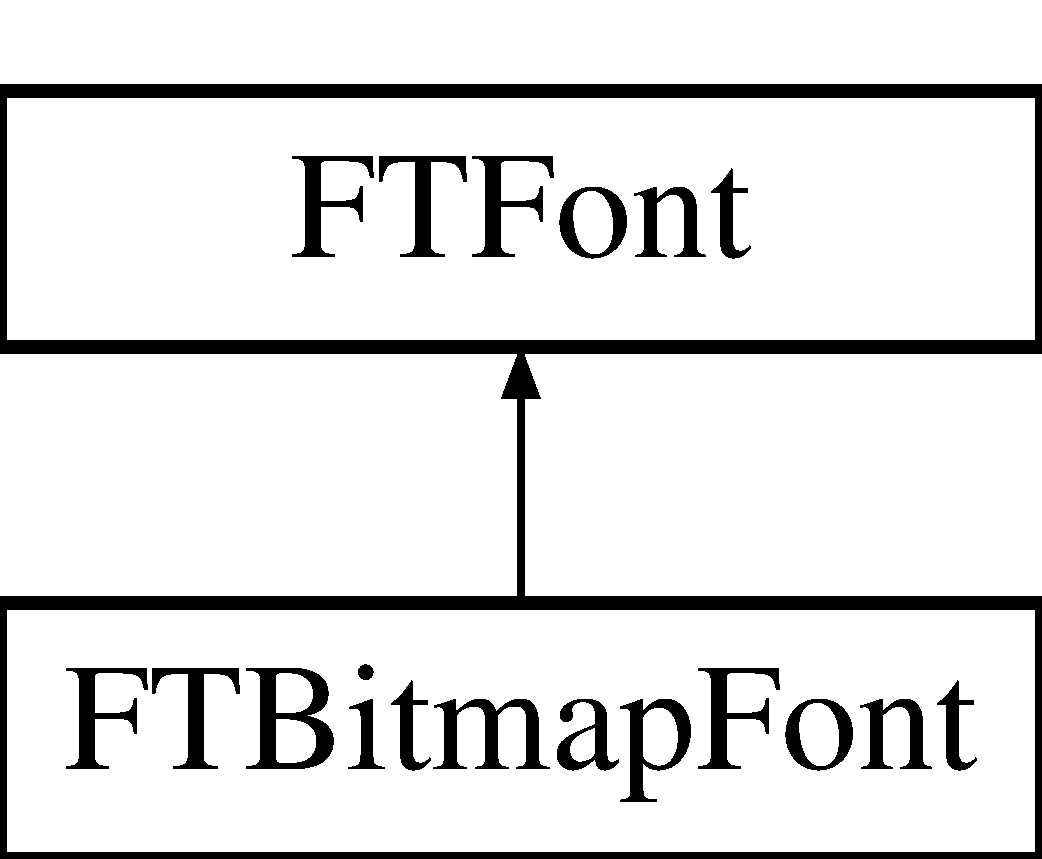
\includegraphics[height=2.000000cm]{classFTBitmapFont}
\end{center}
\end{figure}
\subsection*{Public Member Functions}
\begin{DoxyCompactItemize}
\item 
{\bf FTBitmapFont} (const char $\ast$fontFilePath)
\begin{DoxyCompactList}\small\item\em Open and read a font file. \item\end{DoxyCompactList}\item 
{\bf FTBitmapFont} (const unsigned char $\ast$pBufferBytes, size\_\-t bufferSizeInBytes)
\begin{DoxyCompactList}\small\item\em Open and read a font from a buffer in memory. \item\end{DoxyCompactList}\item 
{\bf $\sim$FTBitmapFont} ()
\begin{DoxyCompactList}\small\item\em Destructor. \item\end{DoxyCompactList}\end{DoxyCompactItemize}
\subsection*{Protected Member Functions}
\begin{DoxyCompactItemize}
\item 
virtual {\bf FTGlyph} $\ast$ {\bf MakeGlyph} (FT\_\-GlyphSlot slot)
\begin{DoxyCompactList}\small\item\em Construct a glyph of the correct type. \item\end{DoxyCompactList}\end{DoxyCompactItemize}


\subsection{Detailed Description}
\doxyref{FTBitmapFont}{p.}{classFTBitmapFont} is a specialisation of the \doxyref{FTFont}{p.}{classFTFont} class for handling Bitmap fonts. \begin{DoxySeeAlso}{See also}
\doxyref{FTFont}{p.}{classFTFont} 
\end{DoxySeeAlso}


Definition at line 45 of file FTGLBitmapFont.h.



\subsection{Constructor \& Destructor Documentation}
\index{FTBitmapFont@{FTBitmapFont}!FTBitmapFont@{FTBitmapFont}}
\index{FTBitmapFont@{FTBitmapFont}!FTBitmapFont@{FTBitmapFont}}
\subsubsection[{FTBitmapFont}]{\setlength{\rightskip}{0pt plus 5cm}FTBitmapFont::FTBitmapFont (
\begin{DoxyParamCaption}
\item[{const char $\ast$}]{ fontFilePath}
\end{DoxyParamCaption}
)}\label{classFTBitmapFont_aa136adf5630071fa6514462b857f6c73}


Open and read a font file. 

Sets Error flag.


\begin{DoxyParams}{Parameters}
{\em fontFilePath} & font file path. \\
\hline
\end{DoxyParams}
\index{FTBitmapFont@{FTBitmapFont}!FTBitmapFont@{FTBitmapFont}}
\index{FTBitmapFont@{FTBitmapFont}!FTBitmapFont@{FTBitmapFont}}
\subsubsection[{FTBitmapFont}]{\setlength{\rightskip}{0pt plus 5cm}FTBitmapFont::FTBitmapFont (
\begin{DoxyParamCaption}
\item[{const unsigned char $\ast$}]{ pBufferBytes, }
\item[{size\_\-t}]{ bufferSizeInBytes}
\end{DoxyParamCaption}
)}\label{classFTBitmapFont_a1163b55f5e90dcab229bd72105a2b1b7}


Open and read a font from a buffer in memory. 

Sets Error flag. The buffer is owned by the client and is NOT copied by \doxyref{FTGL}{p.}{namespaceFTGL}. The pointer must be valid while using \doxyref{FTGL}{p.}{namespaceFTGL}.


\begin{DoxyParams}{Parameters}
{\em pBufferBytes} & the in-\/memory buffer \\
\hline
{\em bufferSizeInBytes} & the length of the buffer in bytes \\
\hline
\end{DoxyParams}
\index{FTBitmapFont@{FTBitmapFont}!$\sim$FTBitmapFont@{$\sim$FTBitmapFont}}
\index{$\sim$FTBitmapFont@{$\sim$FTBitmapFont}!FTBitmapFont@{FTBitmapFont}}
\subsubsection[{$\sim$FTBitmapFont}]{\setlength{\rightskip}{0pt plus 5cm}FTBitmapFont::$\sim$FTBitmapFont (
\begin{DoxyParamCaption}
{}
\end{DoxyParamCaption}
)}\label{classFTBitmapFont_a954ab4a9aea05b83595ac57b4bc3f15d}


Destructor. 



\subsection{Member Function Documentation}
\index{FTBitmapFont@{FTBitmapFont}!MakeGlyph@{MakeGlyph}}
\index{MakeGlyph@{MakeGlyph}!FTBitmapFont@{FTBitmapFont}}
\subsubsection[{MakeGlyph}]{\setlength{\rightskip}{0pt plus 5cm}virtual {\bf FTGlyph}$\ast$ FTBitmapFont::MakeGlyph (
\begin{DoxyParamCaption}
\item[{FT\_\-GlyphSlot}]{ slot}
\end{DoxyParamCaption}
)\hspace{0.3cm}{\ttfamily  [protected, virtual]}}\label{classFTBitmapFont_a4596e73990af0b6e8ab16f94d0915b93}


Construct a glyph of the correct type. 

Clients must override the function and return their specialised \doxyref{FTGlyph}{p.}{classFTGlyph}.


\begin{DoxyParams}{Parameters}
{\em slot} & A FreeType glyph slot. \\
\hline
\end{DoxyParams}
\begin{DoxyReturn}{Returns}
An FT$\ast$$\ast$$\ast$$\ast$Glyph or {\ttfamily null} on failure. 
\end{DoxyReturn}


Implements {\bf FTFont} \doxyref{}{p.}{classFTFont_a07f8bef6c3bd52e7d905e6db17c9b8e6}.



The documentation for this class was generated from the following file:\begin{DoxyCompactItemize}
\item 
{\bf FTGLBitmapFont.h}\end{DoxyCompactItemize}

\section{FTBitmapGlyph Class Reference}
\label{classFTBitmapGlyph}\index{FTBitmapGlyph@{FTBitmapGlyph}}


\doxyref{FTBitmapGlyph}{p.}{classFTBitmapGlyph} is a specialisation of \doxyref{FTGlyph}{p.}{classFTGlyph} for creating bitmaps.  




{\ttfamily \#include $<$FTBitmapGlyph.h$>$}

Inheritance diagram for FTBitmapGlyph:\begin{figure}[H]
\begin{center}
\leavevmode
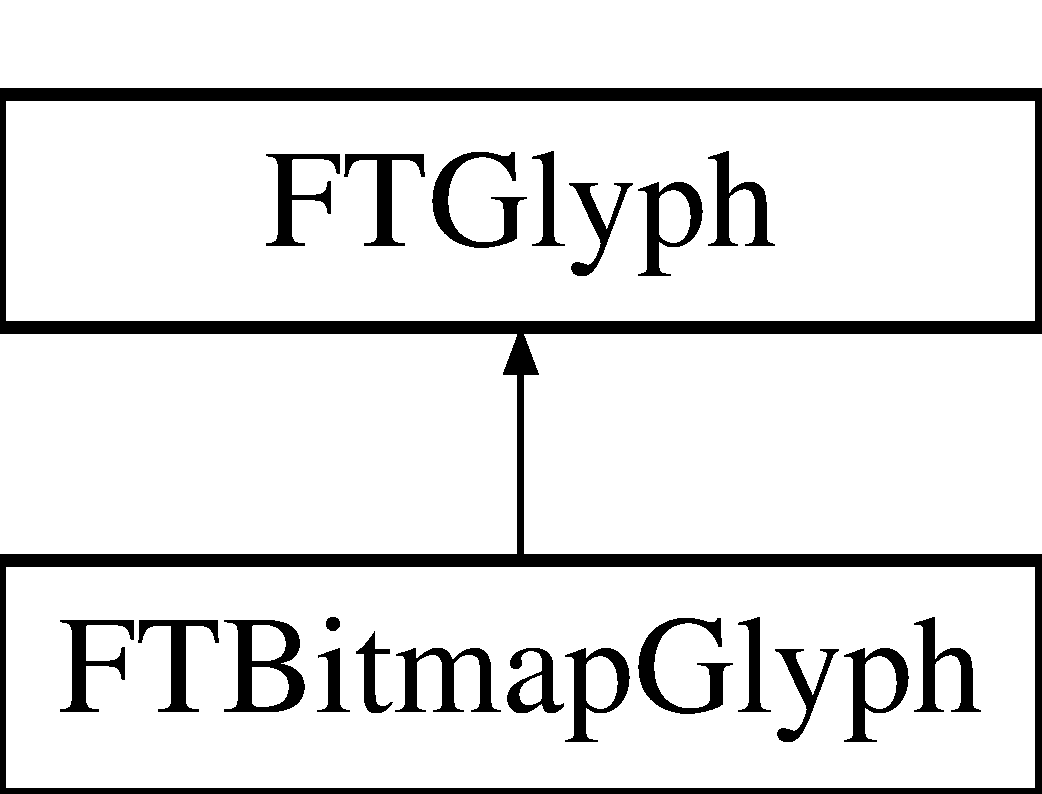
\includegraphics[height=2.000000cm]{classFTBitmapGlyph}
\end{center}
\end{figure}
\subsection*{Public Member Functions}
\begin{DoxyCompactItemize}
\item 
{\bf FTBitmapGlyph} (FT\_\-GlyphSlot glyph)
\begin{DoxyCompactList}\small\item\em Constructor. \item\end{DoxyCompactList}\item 
virtual {\bf $\sim$FTBitmapGlyph} ()
\begin{DoxyCompactList}\small\item\em Destructor. \item\end{DoxyCompactList}\item 
virtual const {\bf FTPoint} \& {\bf Render} (const {\bf FTPoint} \&pen, int renderMode)
\begin{DoxyCompactList}\small\item\em Render this glyph at the current pen position. \item\end{DoxyCompactList}\end{DoxyCompactItemize}


\subsection{Detailed Description}
\doxyref{FTBitmapGlyph}{p.}{classFTBitmapGlyph} is a specialisation of \doxyref{FTGlyph}{p.}{classFTGlyph} for creating bitmaps. 

Definition at line 42 of file FTBitmapGlyph.h.



\subsection{Constructor \& Destructor Documentation}
\index{FTBitmapGlyph@{FTBitmapGlyph}!FTBitmapGlyph@{FTBitmapGlyph}}
\index{FTBitmapGlyph@{FTBitmapGlyph}!FTBitmapGlyph@{FTBitmapGlyph}}
\subsubsection[{FTBitmapGlyph}]{\setlength{\rightskip}{0pt plus 5cm}FTBitmapGlyph::FTBitmapGlyph (
\begin{DoxyParamCaption}
\item[{FT\_\-GlyphSlot}]{ glyph}
\end{DoxyParamCaption}
)}\label{classFTBitmapGlyph_ade810e7077f5f5dd79ef9b2f62a6db56}


Constructor. 


\begin{DoxyParams}{Parameters}
{\em glyph} & The Freetype glyph to be processed \\
\hline
\end{DoxyParams}
\index{FTBitmapGlyph@{FTBitmapGlyph}!$\sim$FTBitmapGlyph@{$\sim$FTBitmapGlyph}}
\index{$\sim$FTBitmapGlyph@{$\sim$FTBitmapGlyph}!FTBitmapGlyph@{FTBitmapGlyph}}
\subsubsection[{$\sim$FTBitmapGlyph}]{\setlength{\rightskip}{0pt plus 5cm}virtual FTBitmapGlyph::$\sim$FTBitmapGlyph (
\begin{DoxyParamCaption}
{}
\end{DoxyParamCaption}
)\hspace{0.3cm}{\ttfamily  [virtual]}}\label{classFTBitmapGlyph_ac5aa31a17033c4a04277a09159466b82}


Destructor. 



\subsection{Member Function Documentation}
\index{FTBitmapGlyph@{FTBitmapGlyph}!Render@{Render}}
\index{Render@{Render}!FTBitmapGlyph@{FTBitmapGlyph}}
\subsubsection[{Render}]{\setlength{\rightskip}{0pt plus 5cm}virtual const {\bf FTPoint}\& FTBitmapGlyph::Render (
\begin{DoxyParamCaption}
\item[{const {\bf FTPoint} \&}]{ pen, }
\item[{int}]{ renderMode}
\end{DoxyParamCaption}
)\hspace{0.3cm}{\ttfamily  [virtual]}}\label{classFTBitmapGlyph_a7286040897f117da9f52023da795de42}


Render this glyph at the current pen position. 


\begin{DoxyParams}{Parameters}
{\em pen} & The current pen position. \\
\hline
{\em renderMode} & Render mode to display \\
\hline
\end{DoxyParams}
\begin{DoxyReturn}{Returns}
The advance distance for this glyph. 
\end{DoxyReturn}


Implements {\bf FTGlyph} \doxyref{}{p.}{classFTGlyph_abcf3aef56d4bf022f6d95d5e287800df}.



The documentation for this class was generated from the following file:\begin{DoxyCompactItemize}
\item 
{\bf FTBitmapGlyph.h}\end{DoxyCompactItemize}

\section{FTBuffer Class Reference}
\label{classFTBuffer}\index{FTBuffer@{FTBuffer}}


\doxyref{FTBuffer}{p.}{classFTBuffer} is a helper class for pixel buffers.  




{\ttfamily \#include $<$FTBuffer.h$>$}

\subsection*{Public Member Functions}
\begin{DoxyCompactItemize}
\item 
{\bf FTBuffer} ()
\begin{DoxyCompactList}\small\item\em Default constructor. \item\end{DoxyCompactList}\item 
{\bf $\sim$FTBuffer} ()
\begin{DoxyCompactList}\small\item\em Destructor. \item\end{DoxyCompactList}\item 
{\bf FTPoint} {\bf Pos} () const 
\begin{DoxyCompactList}\small\item\em Get the pen's position in the buffer. \item\end{DoxyCompactList}\item 
void {\bf Pos} ({\bf FTPoint} arg)
\begin{DoxyCompactList}\small\item\em Set the pen's position in the buffer. \item\end{DoxyCompactList}\item 
void {\bf Size} (int w, int h)
\begin{DoxyCompactList}\small\item\em Set the buffer's size. \item\end{DoxyCompactList}\item 
int {\bf Width} () const 
\begin{DoxyCompactList}\small\item\em Get the buffer's width. \item\end{DoxyCompactList}\item 
int {\bf Height} () const 
\begin{DoxyCompactList}\small\item\em Get the buffer's height. \item\end{DoxyCompactList}\item 
unsigned char $\ast$ {\bf Pixels} () const 
\begin{DoxyCompactList}\small\item\em Get the buffer's direct pixel buffer. \item\end{DoxyCompactList}\end{DoxyCompactItemize}


\subsection{Detailed Description}
\doxyref{FTBuffer}{p.}{classFTBuffer} is a helper class for pixel buffers. It provides the interface between \doxyref{FTBufferFont}{p.}{classFTBufferFont} and \doxyref{FTBufferGlyph}{p.}{classFTBufferGlyph} to optimise rendering operations.

\begin{DoxySeeAlso}{See also}
\doxyref{FTBufferGlyph}{p.}{classFTBufferGlyph} 

\doxyref{FTBufferFont}{p.}{classFTBufferFont} 
\end{DoxySeeAlso}


Definition at line 45 of file FTBuffer.h.



\subsection{Constructor \& Destructor Documentation}
\index{FTBuffer@{FTBuffer}!FTBuffer@{FTBuffer}}
\index{FTBuffer@{FTBuffer}!FTBuffer@{FTBuffer}}
\subsubsection[{FTBuffer}]{\setlength{\rightskip}{0pt plus 5cm}FTBuffer::FTBuffer (
\begin{DoxyParamCaption}
{}
\end{DoxyParamCaption}
)}\label{classFTBuffer_a424fd4161942b61338e72dbe5c4ff74a}


Default constructor. 

\index{FTBuffer@{FTBuffer}!$\sim$FTBuffer@{$\sim$FTBuffer}}
\index{$\sim$FTBuffer@{$\sim$FTBuffer}!FTBuffer@{FTBuffer}}
\subsubsection[{$\sim$FTBuffer}]{\setlength{\rightskip}{0pt plus 5cm}FTBuffer::$\sim$FTBuffer (
\begin{DoxyParamCaption}
{}
\end{DoxyParamCaption}
)}\label{classFTBuffer_a26cbf457816ec8ea07cbc207c10281c6}


Destructor. 



\subsection{Member Function Documentation}
\index{FTBuffer@{FTBuffer}!Height@{Height}}
\index{Height@{Height}!FTBuffer@{FTBuffer}}
\subsubsection[{Height}]{\setlength{\rightskip}{0pt plus 5cm}int FTBuffer::Height (
\begin{DoxyParamCaption}
{}
\end{DoxyParamCaption}
) const\hspace{0.3cm}{\ttfamily  [inline]}}\label{classFTBuffer_a97c058c883b1b6d25242964a025faf0f}


Get the buffer's height. 

\begin{DoxyReturn}{Returns}
The buffer's height, in pixels. 
\end{DoxyReturn}


Definition at line 98 of file FTBuffer.h.

\index{FTBuffer@{FTBuffer}!Pixels@{Pixels}}
\index{Pixels@{Pixels}!FTBuffer@{FTBuffer}}
\subsubsection[{Pixels}]{\setlength{\rightskip}{0pt plus 5cm}unsigned char$\ast$ FTBuffer::Pixels (
\begin{DoxyParamCaption}
{}
\end{DoxyParamCaption}
) const\hspace{0.3cm}{\ttfamily  [inline]}}\label{classFTBuffer_a394321c98ce6bc4f016337cb1e9237fb}


Get the buffer's direct pixel buffer. 

\begin{DoxyReturn}{Returns}
A read-\/write pointer to the buffer's pixels. 
\end{DoxyReturn}


Definition at line 105 of file FTBuffer.h.

\index{FTBuffer@{FTBuffer}!Pos@{Pos}}
\index{Pos@{Pos}!FTBuffer@{FTBuffer}}
\subsubsection[{Pos}]{\setlength{\rightskip}{0pt plus 5cm}void FTBuffer::Pos (
\begin{DoxyParamCaption}
\item[{{\bf FTPoint}}]{ arg}
\end{DoxyParamCaption}
)\hspace{0.3cm}{\ttfamily  [inline]}}\label{classFTBuffer_a97ae51522466bfa08a719f439e0059a0}


Set the pen's position in the buffer. 


\begin{DoxyParams}{Parameters}
{\em arg} & An \doxyref{FTPoint}{p.}{classFTPoint} object with the desired pen's position. \\
\hline
\end{DoxyParams}


Definition at line 73 of file FTBuffer.h.

\index{FTBuffer@{FTBuffer}!Pos@{Pos}}
\index{Pos@{Pos}!FTBuffer@{FTBuffer}}
\subsubsection[{Pos}]{\setlength{\rightskip}{0pt plus 5cm}{\bf FTPoint} FTBuffer::Pos (
\begin{DoxyParamCaption}
{}
\end{DoxyParamCaption}
) const\hspace{0.3cm}{\ttfamily  [inline]}}\label{classFTBuffer_a5b5dedc85576f519bd804bb0e8a6b8a0}


Get the pen's position in the buffer. 

\begin{DoxyReturn}{Returns}
The pen's position as an \doxyref{FTPoint}{p.}{classFTPoint} object. 
\end{DoxyReturn}


Definition at line 63 of file FTBuffer.h.

\index{FTBuffer@{FTBuffer}!Size@{Size}}
\index{Size@{Size}!FTBuffer@{FTBuffer}}
\subsubsection[{Size}]{\setlength{\rightskip}{0pt plus 5cm}void FTBuffer::Size (
\begin{DoxyParamCaption}
\item[{int}]{ w, }
\item[{int}]{ h}
\end{DoxyParamCaption}
)}\label{classFTBuffer_a8b37679226ffbaa187236d7c371efcec}


Set the buffer's size. 


\begin{DoxyParams}{Parameters}
{\em w} & The buffer's desired width, in pixels. \\
\hline
{\em h} & The buffer's desired height, in pixels. \\
\hline
\end{DoxyParams}
\index{FTBuffer@{FTBuffer}!Width@{Width}}
\index{Width@{Width}!FTBuffer@{FTBuffer}}
\subsubsection[{Width}]{\setlength{\rightskip}{0pt plus 5cm}int FTBuffer::Width (
\begin{DoxyParamCaption}
{}
\end{DoxyParamCaption}
) const\hspace{0.3cm}{\ttfamily  [inline]}}\label{classFTBuffer_a19cfff5527c3e04ec59f0cfa295d6abe}


Get the buffer's width. 

\begin{DoxyReturn}{Returns}
The buffer's width, in pixels. 
\end{DoxyReturn}


Definition at line 91 of file FTBuffer.h.



The documentation for this class was generated from the following file:\begin{DoxyCompactItemize}
\item 
{\bf FTBuffer.h}\end{DoxyCompactItemize}

\section{FTBufferFont Class Reference}
\label{classFTBufferFont}\index{FTBufferFont@{FTBufferFont}}


\doxyref{FTBufferFont}{p.}{classFTBufferFont} is a specialisation of the \doxyref{FTFont}{p.}{classFTFont} class for handling memory buffer fonts.  




{\ttfamily \#include $<$FTBufferFont.h$>$}

Inheritance diagram for FTBufferFont:\begin{figure}[H]
\begin{center}
\leavevmode
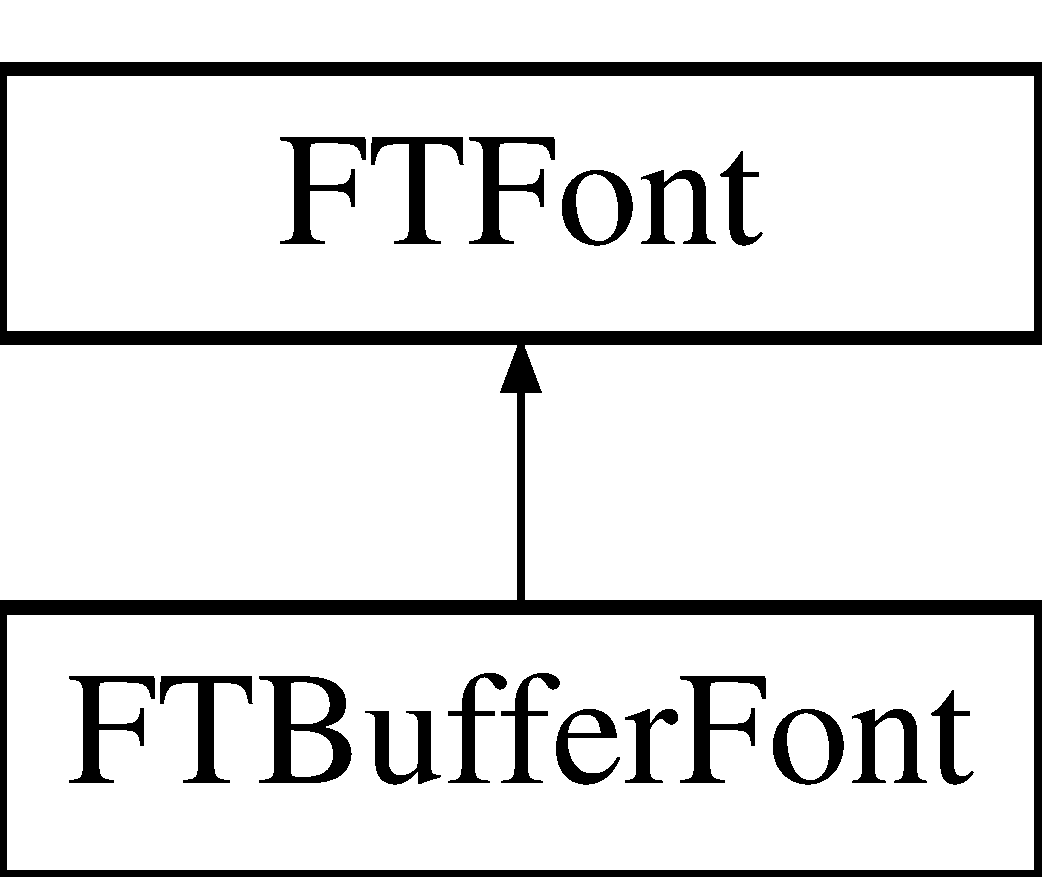
\includegraphics[height=2.000000cm]{classFTBufferFont}
\end{center}
\end{figure}
\subsection*{Public Member Functions}
\begin{DoxyCompactItemize}
\item 
{\bf FTBufferFont} (const char $\ast$fontFilePath)
\begin{DoxyCompactList}\small\item\em Open and read a font file. \item\end{DoxyCompactList}\item 
{\bf FTBufferFont} (const unsigned char $\ast$pBufferBytes, size\_\-t bufferSizeInBytes)
\begin{DoxyCompactList}\small\item\em Open and read a font from a buffer in memory. \item\end{DoxyCompactList}\item 
{\bf $\sim$FTBufferFont} ()
\begin{DoxyCompactList}\small\item\em Destructor. \item\end{DoxyCompactList}\end{DoxyCompactItemize}
\subsection*{Protected Member Functions}
\begin{DoxyCompactItemize}
\item 
virtual {\bf FTGlyph} $\ast$ {\bf MakeGlyph} (FT\_\-GlyphSlot slot)
\begin{DoxyCompactList}\small\item\em Construct a glyph of the correct type. \item\end{DoxyCompactList}\end{DoxyCompactItemize}


\subsection{Detailed Description}
\doxyref{FTBufferFont}{p.}{classFTBufferFont} is a specialisation of the \doxyref{FTFont}{p.}{classFTFont} class for handling memory buffer fonts. \begin{DoxySeeAlso}{See also}
\doxyref{FTFont}{p.}{classFTFont} 
\end{DoxySeeAlso}


Definition at line 43 of file FTBufferFont.h.



\subsection{Constructor \& Destructor Documentation}
\index{FTBufferFont@{FTBufferFont}!FTBufferFont@{FTBufferFont}}
\index{FTBufferFont@{FTBufferFont}!FTBufferFont@{FTBufferFont}}
\subsubsection[{FTBufferFont}]{\setlength{\rightskip}{0pt plus 5cm}FTBufferFont::FTBufferFont (
\begin{DoxyParamCaption}
\item[{const char $\ast$}]{ fontFilePath}
\end{DoxyParamCaption}
)}\label{classFTBufferFont_ad58610385b5ab7d8969623c3d1191485}


Open and read a font file. 

Sets Error flag.


\begin{DoxyParams}{Parameters}
{\em fontFilePath} & font file path. \\
\hline
\end{DoxyParams}
\index{FTBufferFont@{FTBufferFont}!FTBufferFont@{FTBufferFont}}
\index{FTBufferFont@{FTBufferFont}!FTBufferFont@{FTBufferFont}}
\subsubsection[{FTBufferFont}]{\setlength{\rightskip}{0pt plus 5cm}FTBufferFont::FTBufferFont (
\begin{DoxyParamCaption}
\item[{const unsigned char $\ast$}]{ pBufferBytes, }
\item[{size\_\-t}]{ bufferSizeInBytes}
\end{DoxyParamCaption}
)}\label{classFTBufferFont_a30367e01fe57608a95e5f644459390a1}


Open and read a font from a buffer in memory. 

Sets Error flag. The buffer is owned by the client and is NOT copied by \doxyref{FTGL}{p.}{namespaceFTGL}. The pointer must be valid while using \doxyref{FTGL}{p.}{namespaceFTGL}.


\begin{DoxyParams}{Parameters}
{\em pBufferBytes} & the in-\/memory buffer \\
\hline
{\em bufferSizeInBytes} & the length of the buffer in bytes \\
\hline
\end{DoxyParams}
\index{FTBufferFont@{FTBufferFont}!$\sim$FTBufferFont@{$\sim$FTBufferFont}}
\index{$\sim$FTBufferFont@{$\sim$FTBufferFont}!FTBufferFont@{FTBufferFont}}
\subsubsection[{$\sim$FTBufferFont}]{\setlength{\rightskip}{0pt plus 5cm}FTBufferFont::$\sim$FTBufferFont (
\begin{DoxyParamCaption}
{}
\end{DoxyParamCaption}
)}\label{classFTBufferFont_a94d17d98bc86e6dbeda26068b4b8c97f}


Destructor. 



\subsection{Member Function Documentation}
\index{FTBufferFont@{FTBufferFont}!MakeGlyph@{MakeGlyph}}
\index{MakeGlyph@{MakeGlyph}!FTBufferFont@{FTBufferFont}}
\subsubsection[{MakeGlyph}]{\setlength{\rightskip}{0pt plus 5cm}virtual {\bf FTGlyph}$\ast$ FTBufferFont::MakeGlyph (
\begin{DoxyParamCaption}
\item[{FT\_\-GlyphSlot}]{ slot}
\end{DoxyParamCaption}
)\hspace{0.3cm}{\ttfamily  [protected, virtual]}}\label{classFTBufferFont_a8a70fe36e8a627f88cef4dc156fdd2d7}


Construct a glyph of the correct type. 

Clients must override the function and return their specialised \doxyref{FTGlyph}{p.}{classFTGlyph}.


\begin{DoxyParams}{Parameters}
{\em slot} & A FreeType glyph slot. \\
\hline
\end{DoxyParams}
\begin{DoxyReturn}{Returns}
An FT$\ast$$\ast$$\ast$$\ast$Glyph or {\ttfamily null} on failure. 
\end{DoxyReturn}


Implements {\bf FTFont} \doxyref{}{p.}{classFTFont_a07f8bef6c3bd52e7d905e6db17c9b8e6}.



The documentation for this class was generated from the following file:\begin{DoxyCompactItemize}
\item 
{\bf FTBufferFont.h}\end{DoxyCompactItemize}

\section{FTBufferGlyph Class Reference}
\label{classFTBufferGlyph}\index{FTBufferGlyph@{FTBufferGlyph}}


\doxyref{FTBufferGlyph}{p.}{classFTBufferGlyph} is a specialisation of \doxyref{FTGlyph}{p.}{classFTGlyph} for memory buffer rendering.  




{\ttfamily \#include $<$FTBufferGlyph.h$>$}

Inheritance diagram for FTBufferGlyph:\begin{figure}[H]
\begin{center}
\leavevmode
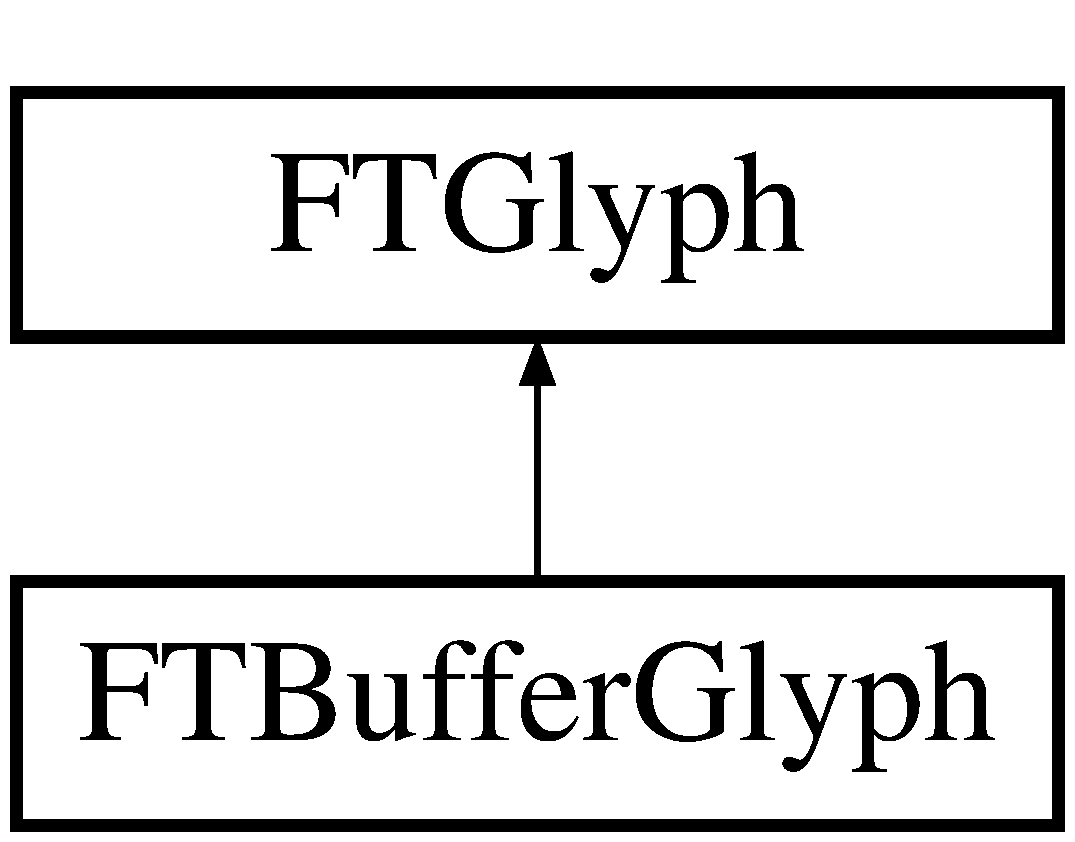
\includegraphics[height=2.000000cm]{classFTBufferGlyph}
\end{center}
\end{figure}
\subsection*{Public Member Functions}
\begin{DoxyCompactItemize}
\item 
{\bf FTBufferGlyph} (FT\_\-GlyphSlot glyph, {\bf FTBuffer} $\ast$buffer)
\begin{DoxyCompactList}\small\item\em Constructor. \item\end{DoxyCompactList}\item 
virtual {\bf $\sim$FTBufferGlyph} ()
\begin{DoxyCompactList}\small\item\em Destructor. \item\end{DoxyCompactList}\item 
virtual const {\bf FTPoint} \& {\bf Render} (const {\bf FTPoint} \&pen, int renderMode)
\begin{DoxyCompactList}\small\item\em Render this glyph at the current pen position. \item\end{DoxyCompactList}\end{DoxyCompactItemize}


\subsection{Detailed Description}
\doxyref{FTBufferGlyph}{p.}{classFTBufferGlyph} is a specialisation of \doxyref{FTGlyph}{p.}{classFTGlyph} for memory buffer rendering. 

Definition at line 40 of file FTBufferGlyph.h.



\subsection{Constructor \& Destructor Documentation}
\index{FTBufferGlyph@{FTBufferGlyph}!FTBufferGlyph@{FTBufferGlyph}}
\index{FTBufferGlyph@{FTBufferGlyph}!FTBufferGlyph@{FTBufferGlyph}}
\subsubsection[{FTBufferGlyph}]{\setlength{\rightskip}{0pt plus 5cm}FTBufferGlyph::FTBufferGlyph (
\begin{DoxyParamCaption}
\item[{FT\_\-GlyphSlot}]{ glyph, }
\item[{{\bf FTBuffer} $\ast$}]{ buffer}
\end{DoxyParamCaption}
)}\label{classFTBufferGlyph_a48b9e99cb65964ae32776f26da65c25e}


Constructor. 


\begin{DoxyParams}{Parameters}
{\em glyph} & The Freetype glyph to be processed \\
\hline
{\em buffer} & An \doxyref{FTBuffer}{p.}{classFTBuffer} object in which to render the glyph. \\
\hline
\end{DoxyParams}
\index{FTBufferGlyph@{FTBufferGlyph}!$\sim$FTBufferGlyph@{$\sim$FTBufferGlyph}}
\index{$\sim$FTBufferGlyph@{$\sim$FTBufferGlyph}!FTBufferGlyph@{FTBufferGlyph}}
\subsubsection[{$\sim$FTBufferGlyph}]{\setlength{\rightskip}{0pt plus 5cm}virtual FTBufferGlyph::$\sim$FTBufferGlyph (
\begin{DoxyParamCaption}
{}
\end{DoxyParamCaption}
)\hspace{0.3cm}{\ttfamily  [virtual]}}\label{classFTBufferGlyph_ab87dedb20a3216d24535958e2f2e0460}


Destructor. 



\subsection{Member Function Documentation}
\index{FTBufferGlyph@{FTBufferGlyph}!Render@{Render}}
\index{Render@{Render}!FTBufferGlyph@{FTBufferGlyph}}
\subsubsection[{Render}]{\setlength{\rightskip}{0pt plus 5cm}virtual const {\bf FTPoint}\& FTBufferGlyph::Render (
\begin{DoxyParamCaption}
\item[{const {\bf FTPoint} \&}]{ pen, }
\item[{int}]{ renderMode}
\end{DoxyParamCaption}
)\hspace{0.3cm}{\ttfamily  [virtual]}}\label{classFTBufferGlyph_a33bc5176b9c5739f20d634eca04a45a5}


Render this glyph at the current pen position. 


\begin{DoxyParams}{Parameters}
{\em pen} & The current pen position. \\
\hline
{\em renderMode} & Render mode to display \\
\hline
\end{DoxyParams}
\begin{DoxyReturn}{Returns}
The advance distance for this glyph. 
\end{DoxyReturn}


Implements {\bf FTGlyph} \doxyref{}{p.}{classFTGlyph_abcf3aef56d4bf022f6d95d5e287800df}.



The documentation for this class was generated from the following file:\begin{DoxyCompactItemize}
\item 
{\bf FTBufferGlyph.h}\end{DoxyCompactItemize}

\section{FTExtrudeFont Class Reference}
\label{classFTExtrudeFont}\index{FTExtrudeFont@{FTExtrudeFont}}


\doxyref{FTExtrudeFont}{p.}{classFTExtrudeFont} is a specialisation of the \doxyref{FTFont}{p.}{classFTFont} class for handling extruded Polygon fonts.  




{\ttfamily \#include $<$FTGLExtrdFont.h$>$}

Inheritance diagram for FTExtrudeFont:\begin{figure}[H]
\begin{center}
\leavevmode
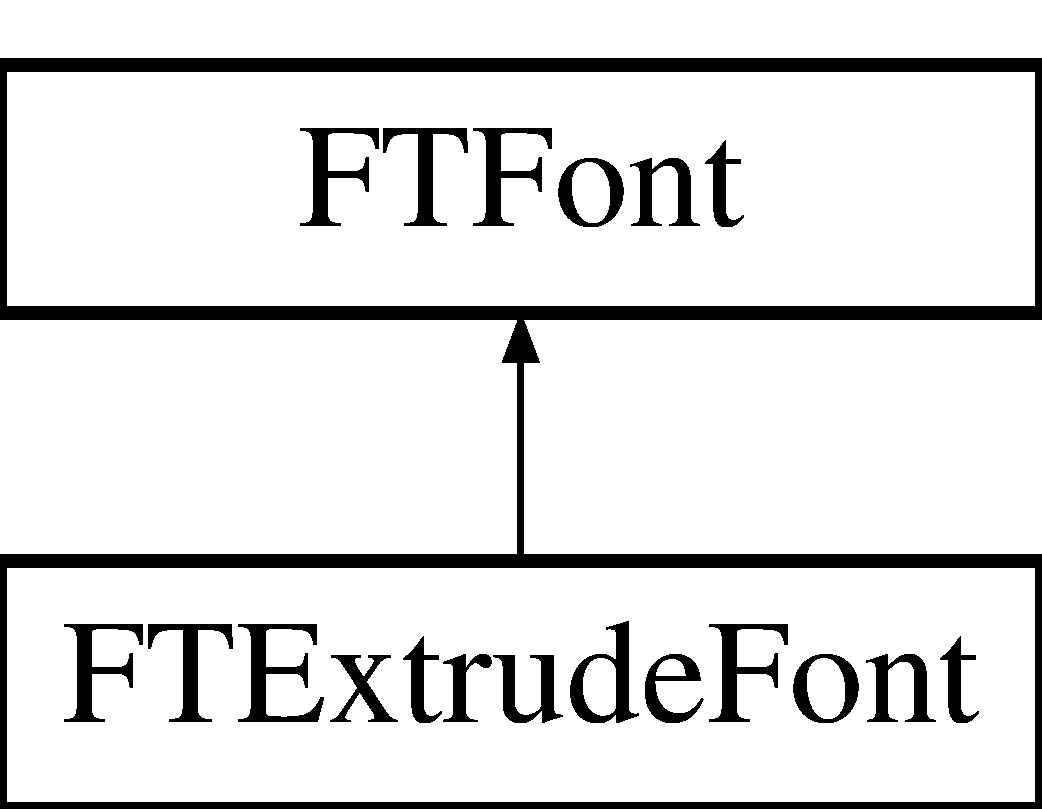
\includegraphics[height=2.000000cm]{classFTExtrudeFont}
\end{center}
\end{figure}
\subsection*{Public Member Functions}
\begin{DoxyCompactItemize}
\item 
{\bf FTExtrudeFont} (const char $\ast$fontFilePath)
\begin{DoxyCompactList}\small\item\em Open and read a font file. \item\end{DoxyCompactList}\item 
{\bf FTExtrudeFont} (const unsigned char $\ast$pBufferBytes, size\_\-t bufferSizeInBytes)
\begin{DoxyCompactList}\small\item\em Open and read a font from a buffer in memory. \item\end{DoxyCompactList}\item 
{\bf $\sim$FTExtrudeFont} ()
\begin{DoxyCompactList}\small\item\em Destructor. \item\end{DoxyCompactList}\end{DoxyCompactItemize}
\subsection*{Protected Member Functions}
\begin{DoxyCompactItemize}
\item 
virtual {\bf FTGlyph} $\ast$ {\bf MakeGlyph} (FT\_\-GlyphSlot slot)
\begin{DoxyCompactList}\small\item\em Construct a glyph of the correct type. \item\end{DoxyCompactList}\end{DoxyCompactItemize}


\subsection{Detailed Description}
\doxyref{FTExtrudeFont}{p.}{classFTExtrudeFont} is a specialisation of the \doxyref{FTFont}{p.}{classFTFont} class for handling extruded Polygon fonts. \begin{DoxySeeAlso}{See also}
\doxyref{FTFont}{p.}{classFTFont} 

\doxyref{FTPolygonFont}{p.}{classFTPolygonFont} 
\end{DoxySeeAlso}


Definition at line 46 of file FTGLExtrdFont.h.



\subsection{Constructor \& Destructor Documentation}
\index{FTExtrudeFont@{FTExtrudeFont}!FTExtrudeFont@{FTExtrudeFont}}
\index{FTExtrudeFont@{FTExtrudeFont}!FTExtrudeFont@{FTExtrudeFont}}
\subsubsection[{FTExtrudeFont}]{\setlength{\rightskip}{0pt plus 5cm}FTExtrudeFont::FTExtrudeFont (
\begin{DoxyParamCaption}
\item[{const char $\ast$}]{ fontFilePath}
\end{DoxyParamCaption}
)}\label{classFTExtrudeFont_a9c1d32ca35a021629bc7c7039fdba359}


Open and read a font file. 

Sets Error flag.


\begin{DoxyParams}{Parameters}
{\em fontFilePath} & font file path. \\
\hline
\end{DoxyParams}
\index{FTExtrudeFont@{FTExtrudeFont}!FTExtrudeFont@{FTExtrudeFont}}
\index{FTExtrudeFont@{FTExtrudeFont}!FTExtrudeFont@{FTExtrudeFont}}
\subsubsection[{FTExtrudeFont}]{\setlength{\rightskip}{0pt plus 5cm}FTExtrudeFont::FTExtrudeFont (
\begin{DoxyParamCaption}
\item[{const unsigned char $\ast$}]{ pBufferBytes, }
\item[{size\_\-t}]{ bufferSizeInBytes}
\end{DoxyParamCaption}
)}\label{classFTExtrudeFont_a277554f3390671132f43432c426b8b4d}


Open and read a font from a buffer in memory. 

Sets Error flag. The buffer is owned by the client and is NOT copied by \doxyref{FTGL}{p.}{namespaceFTGL}. The pointer must be valid while using \doxyref{FTGL}{p.}{namespaceFTGL}.


\begin{DoxyParams}{Parameters}
{\em pBufferBytes} & the in-\/memory buffer \\
\hline
{\em bufferSizeInBytes} & the length of the buffer in bytes \\
\hline
\end{DoxyParams}
\index{FTExtrudeFont@{FTExtrudeFont}!$\sim$FTExtrudeFont@{$\sim$FTExtrudeFont}}
\index{$\sim$FTExtrudeFont@{$\sim$FTExtrudeFont}!FTExtrudeFont@{FTExtrudeFont}}
\subsubsection[{$\sim$FTExtrudeFont}]{\setlength{\rightskip}{0pt plus 5cm}FTExtrudeFont::$\sim$FTExtrudeFont (
\begin{DoxyParamCaption}
{}
\end{DoxyParamCaption}
)}\label{classFTExtrudeFont_af5dcb9d91f560903353bd6ac445bbb04}


Destructor. 



\subsection{Member Function Documentation}
\index{FTExtrudeFont@{FTExtrudeFont}!MakeGlyph@{MakeGlyph}}
\index{MakeGlyph@{MakeGlyph}!FTExtrudeFont@{FTExtrudeFont}}
\subsubsection[{MakeGlyph}]{\setlength{\rightskip}{0pt plus 5cm}virtual {\bf FTGlyph}$\ast$ FTExtrudeFont::MakeGlyph (
\begin{DoxyParamCaption}
\item[{FT\_\-GlyphSlot}]{ slot}
\end{DoxyParamCaption}
)\hspace{0.3cm}{\ttfamily  [protected, virtual]}}\label{classFTExtrudeFont_a096fcfe612dc98f49dbc818ac47d2680}


Construct a glyph of the correct type. 

Clients must override the function and return their specialised \doxyref{FTGlyph}{p.}{classFTGlyph}.


\begin{DoxyParams}{Parameters}
{\em slot} & A FreeType glyph slot. \\
\hline
\end{DoxyParams}
\begin{DoxyReturn}{Returns}
An FT$\ast$$\ast$$\ast$$\ast$Glyph or {\ttfamily null} on failure. 
\end{DoxyReturn}


Implements {\bf FTFont} \doxyref{}{p.}{classFTFont_a07f8bef6c3bd52e7d905e6db17c9b8e6}.



The documentation for this class was generated from the following file:\begin{DoxyCompactItemize}
\item 
{\bf FTGLExtrdFont.h}\end{DoxyCompactItemize}

\section{FTExtrudeGlyph Class Reference}
\label{classFTExtrudeGlyph}\index{FTExtrudeGlyph@{FTExtrudeGlyph}}


\doxyref{FTExtrudeGlyph}{p.}{classFTExtrudeGlyph} is a specialisation of \doxyref{FTGlyph}{p.}{classFTGlyph} for creating tessellated extruded polygon glyphs.  




{\ttfamily \#include $<$FTExtrdGlyph.h$>$}

Inheritance diagram for FTExtrudeGlyph:\begin{figure}[H]
\begin{center}
\leavevmode
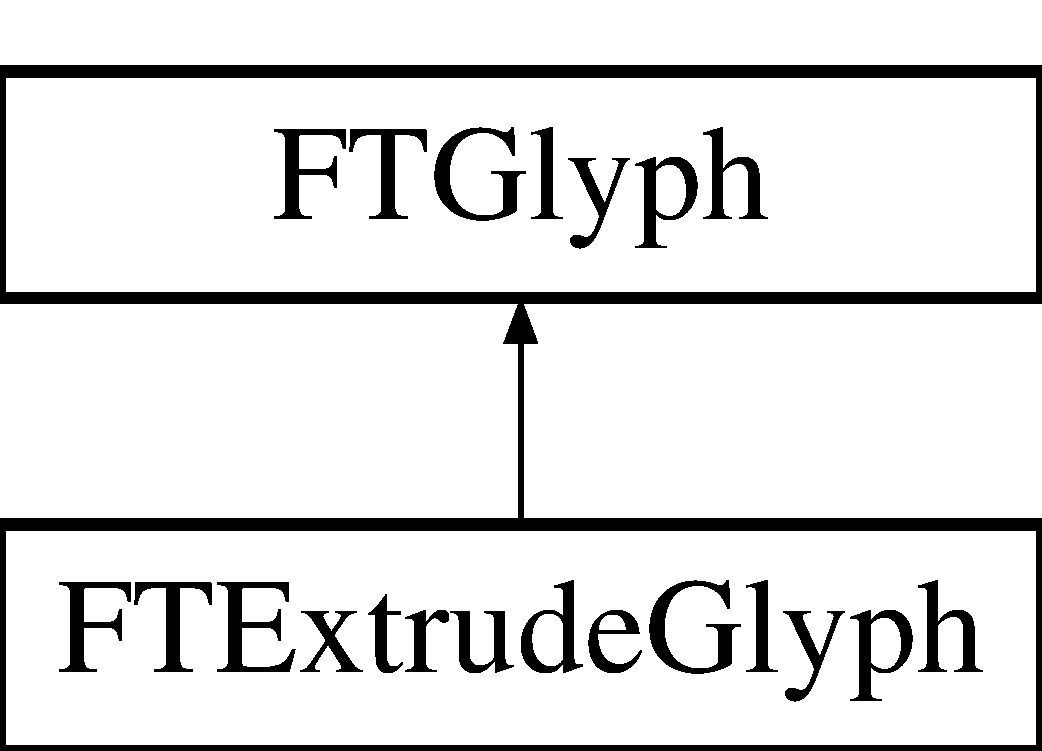
\includegraphics[height=2.000000cm]{classFTExtrudeGlyph}
\end{center}
\end{figure}
\subsection*{Public Member Functions}
\begin{DoxyCompactItemize}
\item 
{\bf FTExtrudeGlyph} (FT\_\-GlyphSlot glyph, float depth, float frontOutset, float backOutset, bool useDisplayList)
\begin{DoxyCompactList}\small\item\em Constructor. \item\end{DoxyCompactList}\item 
virtual {\bf $\sim$FTExtrudeGlyph} ()
\begin{DoxyCompactList}\small\item\em Destructor. \item\end{DoxyCompactList}\item 
virtual const {\bf FTPoint} \& {\bf Render} (const {\bf FTPoint} \&pen, int renderMode)
\begin{DoxyCompactList}\small\item\em Render this glyph at the current pen position. \item\end{DoxyCompactList}\end{DoxyCompactItemize}


\subsection{Detailed Description}
\doxyref{FTExtrudeGlyph}{p.}{classFTExtrudeGlyph} is a specialisation of \doxyref{FTGlyph}{p.}{classFTGlyph} for creating tessellated extruded polygon glyphs. 

Definition at line 43 of file FTExtrdGlyph.h.



\subsection{Constructor \& Destructor Documentation}
\index{FTExtrudeGlyph@{FTExtrudeGlyph}!FTExtrudeGlyph@{FTExtrudeGlyph}}
\index{FTExtrudeGlyph@{FTExtrudeGlyph}!FTExtrudeGlyph@{FTExtrudeGlyph}}
\subsubsection[{FTExtrudeGlyph}]{\setlength{\rightskip}{0pt plus 5cm}FTExtrudeGlyph::FTExtrudeGlyph (
\begin{DoxyParamCaption}
\item[{FT\_\-GlyphSlot}]{ glyph, }
\item[{float}]{ depth, }
\item[{float}]{ frontOutset, }
\item[{float}]{ backOutset, }
\item[{bool}]{ useDisplayList}
\end{DoxyParamCaption}
)}\label{classFTExtrudeGlyph_a76ca3fac3f26bf967b98464d306778cd}


Constructor. 

Sets the Error to Invalid\_\-Outline if the glyph isn't an outline.


\begin{DoxyParams}{Parameters}
{\em glyph} & The Freetype glyph to be processed \\
\hline
{\em depth} & The distance along the z axis to extrude the glyph \\
\hline
{\em frontOutset} & outset contour size \\
\hline
{\em backOutset} & outset contour size \\
\hline
{\em useDisplayList} & Enable or disable the use of Display Lists for this glyph {\ttfamily true} turns ON display lists. {\ttfamily false} turns OFF display lists. \\
\hline
\end{DoxyParams}
\index{FTExtrudeGlyph@{FTExtrudeGlyph}!$\sim$FTExtrudeGlyph@{$\sim$FTExtrudeGlyph}}
\index{$\sim$FTExtrudeGlyph@{$\sim$FTExtrudeGlyph}!FTExtrudeGlyph@{FTExtrudeGlyph}}
\subsubsection[{$\sim$FTExtrudeGlyph}]{\setlength{\rightskip}{0pt plus 5cm}virtual FTExtrudeGlyph::$\sim$FTExtrudeGlyph (
\begin{DoxyParamCaption}
{}
\end{DoxyParamCaption}
)\hspace{0.3cm}{\ttfamily  [virtual]}}\label{classFTExtrudeGlyph_af83d3b160cd5cccea8c3fc343be7a9b3}


Destructor. 



\subsection{Member Function Documentation}
\index{FTExtrudeGlyph@{FTExtrudeGlyph}!Render@{Render}}
\index{Render@{Render}!FTExtrudeGlyph@{FTExtrudeGlyph}}
\subsubsection[{Render}]{\setlength{\rightskip}{0pt plus 5cm}virtual const {\bf FTPoint}\& FTExtrudeGlyph::Render (
\begin{DoxyParamCaption}
\item[{const {\bf FTPoint} \&}]{ pen, }
\item[{int}]{ renderMode}
\end{DoxyParamCaption}
)\hspace{0.3cm}{\ttfamily  [virtual]}}\label{classFTExtrudeGlyph_a48cc5da5e2e6491d79bcee8a9107bc60}


Render this glyph at the current pen position. 


\begin{DoxyParams}{Parameters}
{\em pen} & The current pen position. \\
\hline
{\em renderMode} & Render mode to display \\
\hline
\end{DoxyParams}
\begin{DoxyReturn}{Returns}
The advance distance for this glyph. 
\end{DoxyReturn}


Implements {\bf FTGlyph} \doxyref{}{p.}{classFTGlyph_abcf3aef56d4bf022f6d95d5e287800df}.



The documentation for this class was generated from the following file:\begin{DoxyCompactItemize}
\item 
{\bf FTExtrdGlyph.h}\end{DoxyCompactItemize}

\section{FTFont Class Reference}
\label{classFTFont}\index{FTFont@{FTFont}}


\doxyref{FTFont}{p.}{classFTFont} is the public interface for the \doxyref{FTGL}{p.}{namespaceFTGL} library.  




{\ttfamily \#include $<$FTFont.h$>$}

Inheritance diagram for FTFont:\begin{figure}[H]
\begin{center}
\leavevmode
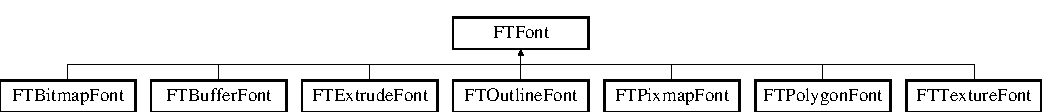
\includegraphics[height=1.509434cm]{classFTFont}
\end{center}
\end{figure}
\subsection*{Public Member Functions}
\begin{DoxyCompactItemize}
\item 
virtual {\bf $\sim$FTFont} ()
\item 
virtual bool {\bf Attach} (const char $\ast$fontFilePath)
\begin{DoxyCompactList}\small\item\em Attach auxilliary file to font e.g font metrics. \item\end{DoxyCompactList}\item 
virtual bool {\bf Attach} (const unsigned char $\ast$pBufferBytes, size\_\-t bufferSizeInBytes)
\begin{DoxyCompactList}\small\item\em Attach auxilliary data to font e.g font metrics, from memory. \item\end{DoxyCompactList}\item 
virtual void {\bf GlyphLoadFlags} (FT\_\-Int flags)
\begin{DoxyCompactList}\small\item\em Set the glyph loading flags. \item\end{DoxyCompactList}\item 
virtual bool {\bf CharMap} (FT\_\-Encoding encoding)
\begin{DoxyCompactList}\small\item\em Set the character map for the face. \item\end{DoxyCompactList}\item 
virtual unsigned int {\bf CharMapCount} () const 
\begin{DoxyCompactList}\small\item\em Get the number of character maps in this face. \item\end{DoxyCompactList}\item 
virtual FT\_\-Encoding $\ast$ {\bf CharMapList} ()
\begin{DoxyCompactList}\small\item\em Get a list of character maps in this face. \item\end{DoxyCompactList}\item 
virtual bool {\bf FaceSize} (const unsigned int size, const unsigned int res=72)
\begin{DoxyCompactList}\small\item\em Set the char size for the current face. \item\end{DoxyCompactList}\item 
virtual unsigned int {\bf FaceSize} () const 
\begin{DoxyCompactList}\small\item\em Get the current face size in points (1/72 inch). \item\end{DoxyCompactList}\item 
virtual void {\bf Depth} (float depth)
\begin{DoxyCompactList}\small\item\em Set the extrusion distance for the font. \item\end{DoxyCompactList}\item 
virtual void {\bf Outset} (float outset)
\begin{DoxyCompactList}\small\item\em Set the outset distance for the font. \item\end{DoxyCompactList}\item 
virtual void {\bf Outset} (float front, float back)
\begin{DoxyCompactList}\small\item\em Set the front and back outset distances for the font. \item\end{DoxyCompactList}\item 
virtual void {\bf UseDisplayList} (bool useList)
\begin{DoxyCompactList}\small\item\em Enable or disable the use of Display Lists inside \doxyref{FTGL}{p.}{namespaceFTGL}. \item\end{DoxyCompactList}\item 
virtual float {\bf Ascender} () const 
\begin{DoxyCompactList}\small\item\em Get the global ascender height for the face. \item\end{DoxyCompactList}\item 
virtual float {\bf Descender} () const 
\begin{DoxyCompactList}\small\item\em Gets the global descender height for the face. \item\end{DoxyCompactList}\item 
virtual float {\bf LineHeight} () const 
\begin{DoxyCompactList}\small\item\em Gets the line spacing for the font. \item\end{DoxyCompactList}\item 
virtual {\bf FTBBox} {\bf BBox} (const char $\ast$string, const int len=-\/1, {\bf FTPoint} position={\bf FTPoint}(), {\bf FTPoint} spacing={\bf FTPoint}())
\begin{DoxyCompactList}\small\item\em Get the bounding box for a string. \item\end{DoxyCompactList}\item 
void {\bf BBox} (const char $\ast$string, float \&llx, float \&lly, float \&llz, float \&urx, float \&ury, float \&urz)
\begin{DoxyCompactList}\small\item\em Get the bounding box for a string (deprecated). \item\end{DoxyCompactList}\item 
virtual {\bf FTBBox} {\bf BBox} (const wchar\_\-t $\ast$string, const int len=-\/1, {\bf FTPoint} position={\bf FTPoint}(), {\bf FTPoint} spacing={\bf FTPoint}())
\begin{DoxyCompactList}\small\item\em Get the bounding box for a string. \item\end{DoxyCompactList}\item 
void {\bf BBox} (const wchar\_\-t $\ast$string, float \&llx, float \&lly, float \&llz, float \&urx, float \&ury, float \&urz)
\begin{DoxyCompactList}\small\item\em Get the bounding box for a string (deprecated). \item\end{DoxyCompactList}\item 
virtual float {\bf Advance} (const char $\ast$string, const int len=-\/1, {\bf FTPoint} spacing={\bf FTPoint}())
\begin{DoxyCompactList}\small\item\em Get the advance for a string. \item\end{DoxyCompactList}\item 
virtual float {\bf Advance} (const wchar\_\-t $\ast$string, const int len=-\/1, {\bf FTPoint} spacing={\bf FTPoint}())
\begin{DoxyCompactList}\small\item\em Get the advance for a string. \item\end{DoxyCompactList}\item 
virtual {\bf FTPoint} {\bf Render} (const char $\ast$string, const int len=-\/1, {\bf FTPoint} position={\bf FTPoint}(), {\bf FTPoint} spacing={\bf FTPoint}(), int renderMode=FTGL::RENDER\_\-ALL)
\begin{DoxyCompactList}\small\item\em Render a string of characters. \item\end{DoxyCompactList}\item 
virtual {\bf FTPoint} {\bf Render} (const wchar\_\-t $\ast$string, const int len=-\/1, {\bf FTPoint} position={\bf FTPoint}(), {\bf FTPoint} spacing={\bf FTPoint}(), int renderMode=FTGL::RENDER\_\-ALL)
\begin{DoxyCompactList}\small\item\em Render a string of characters. \item\end{DoxyCompactList}\item 
virtual FT\_\-Error {\bf Error} () const 
\begin{DoxyCompactList}\small\item\em Queries the Font for errors. \item\end{DoxyCompactList}\end{DoxyCompactItemize}
\subsection*{Protected Member Functions}
\begin{DoxyCompactItemize}
\item 
{\bf FTFont} (char const $\ast$fontFilePath)
\begin{DoxyCompactList}\small\item\em Open and read a font file. \item\end{DoxyCompactList}\item 
{\bf FTFont} (const unsigned char $\ast$pBufferBytes, size\_\-t bufferSizeInBytes)
\begin{DoxyCompactList}\small\item\em Open and read a font from a buffer in memory. \item\end{DoxyCompactList}\item 
virtual {\bf FTGlyph} $\ast$ {\bf MakeGlyph} (FT\_\-GlyphSlot slot)=0
\begin{DoxyCompactList}\small\item\em Construct a glyph of the correct type. \item\end{DoxyCompactList}\end{DoxyCompactItemize}
\subsection*{Friends}
\begin{DoxyCompactItemize}
\item 
class {\bf FTBitmapFont}
\item 
class {\bf FTBufferFont}
\item 
class {\bf FTExtrudeFont}
\item 
class {\bf FTOutlineFont}
\item 
class {\bf FTPixmapFont}
\item 
class {\bf FTPolygonFont}
\item 
class {\bf FTTextureFont}
\item 
class {\bf FTFontImpl}
\end{DoxyCompactItemize}


\subsection{Detailed Description}
\doxyref{FTFont}{p.}{classFTFont} is the public interface for the \doxyref{FTGL}{p.}{namespaceFTGL} library. Specific font classes are derived from this class. It uses the helper classes FTFace and FTSize to access the Freetype library. This class is abstract and deriving classes must implement the protected {\ttfamily MakeGlyph} function to create glyphs of the appropriate type.

It is good practice after using these functions to test the error code returned. {\ttfamily FT\_\-Error \doxyref{Error()}{p.}{classFTFont_a1b535e3a7fef84c073988ab6f74f9ec1}}. Check the freetype file fterrdef.h for error definitions.

\begin{DoxySeeAlso}{See also}
FTFace 

FTSize 
\end{DoxySeeAlso}


Definition at line 56 of file FTFont.h.



\subsection{Constructor \& Destructor Documentation}
\index{FTFont@{FTFont}!FTFont@{FTFont}}
\index{FTFont@{FTFont}!FTFont@{FTFont}}
\subsubsection[{FTFont}]{\setlength{\rightskip}{0pt plus 5cm}FTFont::FTFont (
\begin{DoxyParamCaption}
\item[{char const $\ast$}]{ fontFilePath}
\end{DoxyParamCaption}
)\hspace{0.3cm}{\ttfamily  [protected]}}\label{classFTFont_af7edeab8bc77784a537dc63e54315cc9}


Open and read a font file. 

Sets Error flag.


\begin{DoxyParams}{Parameters}
{\em fontFilePath} & font file path. \\
\hline
\end{DoxyParams}
\index{FTFont@{FTFont}!FTFont@{FTFont}}
\index{FTFont@{FTFont}!FTFont@{FTFont}}
\subsubsection[{FTFont}]{\setlength{\rightskip}{0pt plus 5cm}FTFont::FTFont (
\begin{DoxyParamCaption}
\item[{const unsigned char $\ast$}]{ pBufferBytes, }
\item[{size\_\-t}]{ bufferSizeInBytes}
\end{DoxyParamCaption}
)\hspace{0.3cm}{\ttfamily  [protected]}}\label{classFTFont_a8911254ec56e3b9c36891459b98beaf2}


Open and read a font from a buffer in memory. 

Sets Error flag. The buffer is owned by the client and is NOT copied by \doxyref{FTGL}{p.}{namespaceFTGL}. The pointer must be valid while using \doxyref{FTGL}{p.}{namespaceFTGL}.


\begin{DoxyParams}{Parameters}
{\em pBufferBytes} & the in-\/memory buffer \\
\hline
{\em bufferSizeInBytes} & the length of the buffer in bytes \\
\hline
\end{DoxyParams}
\index{FTFont@{FTFont}!$\sim$FTFont@{$\sim$FTFont}}
\index{$\sim$FTFont@{$\sim$FTFont}!FTFont@{FTFont}}
\subsubsection[{$\sim$FTFont}]{\setlength{\rightskip}{0pt plus 5cm}virtual FTFont::$\sim$FTFont (
\begin{DoxyParamCaption}
{}
\end{DoxyParamCaption}
)\hspace{0.3cm}{\ttfamily  [virtual]}}\label{classFTFont_a9df9b873c582024867ff6b9dfff0face}


\subsection{Member Function Documentation}
\index{FTFont@{FTFont}!Advance@{Advance}}
\index{Advance@{Advance}!FTFont@{FTFont}}
\subsubsection[{Advance}]{\setlength{\rightskip}{0pt plus 5cm}virtual float FTFont::Advance (
\begin{DoxyParamCaption}
\item[{const char $\ast$}]{ string, }
\item[{const int}]{ len = {\ttfamily -\/1}, }
\item[{{\bf FTPoint}}]{ spacing = {\ttfamily {\bf FTPoint}()}}
\end{DoxyParamCaption}
)\hspace{0.3cm}{\ttfamily  [virtual]}}\label{classFTFont_ae606eb0323341d1a521dae7a712f1b6e}


Get the advance for a string. 


\begin{DoxyParams}{Parameters}
{\em string} & 'C' style string to be checked. \\
\hline
{\em len} & The length of the string. If $<$ 0 then all characters will be checked until a null character is encountered (optional). \\
\hline
{\em spacing} & A displacement vector to add after each character has been checked (optional). \\
\hline
\end{DoxyParams}
\begin{DoxyReturn}{Returns}
The string's advance width. 
\end{DoxyReturn}
\index{FTFont@{FTFont}!Advance@{Advance}}
\index{Advance@{Advance}!FTFont@{FTFont}}
\subsubsection[{Advance}]{\setlength{\rightskip}{0pt plus 5cm}virtual float FTFont::Advance (
\begin{DoxyParamCaption}
\item[{const wchar\_\-t $\ast$}]{ string, }
\item[{const int}]{ len = {\ttfamily -\/1}, }
\item[{{\bf FTPoint}}]{ spacing = {\ttfamily {\bf FTPoint}()}}
\end{DoxyParamCaption}
)\hspace{0.3cm}{\ttfamily  [virtual]}}\label{classFTFont_a030a33368ab7fcbcb082909e4c2d6b89}


Get the advance for a string. 


\begin{DoxyParams}{Parameters}
{\em string} & A wchar\_\-t string \\
\hline
{\em len} & The length of the string. If $<$ 0 then all characters will be checked until a null character is encountered (optional). \\
\hline
{\em spacing} & A displacement vector to add after each character has been checked (optional). \\
\hline
\end{DoxyParams}
\begin{DoxyReturn}{Returns}
The string's advance width. 
\end{DoxyReturn}
\index{FTFont@{FTFont}!Ascender@{Ascender}}
\index{Ascender@{Ascender}!FTFont@{FTFont}}
\subsubsection[{Ascender}]{\setlength{\rightskip}{0pt plus 5cm}virtual float FTFont::Ascender (
\begin{DoxyParamCaption}
{}
\end{DoxyParamCaption}
) const\hspace{0.3cm}{\ttfamily  [virtual]}}\label{classFTFont_ac4659028a0be30e8bc85814e7e53ee87}


Get the global ascender height for the face. 

\begin{DoxyReturn}{Returns}
Ascender height 
\end{DoxyReturn}
\index{FTFont@{FTFont}!Attach@{Attach}}
\index{Attach@{Attach}!FTFont@{FTFont}}
\subsubsection[{Attach}]{\setlength{\rightskip}{0pt plus 5cm}virtual bool FTFont::Attach (
\begin{DoxyParamCaption}
\item[{const unsigned char $\ast$}]{ pBufferBytes, }
\item[{size\_\-t}]{ bufferSizeInBytes}
\end{DoxyParamCaption}
)\hspace{0.3cm}{\ttfamily  [virtual]}}\label{classFTFont_a95f86388d8cb2ba1c94679d30c68aba5}


Attach auxilliary data to font e.g font metrics, from memory. 

Note: not all font formats implement this function.


\begin{DoxyParams}{Parameters}
{\em pBufferBytes} & the in-\/memory buffer. \\
\hline
{\em bufferSizeInBytes} & the length of the buffer in bytes. \\
\hline
\end{DoxyParams}
\begin{DoxyReturn}{Returns}
{\ttfamily true} if file has been attached successfully. 
\end{DoxyReturn}
\index{FTFont@{FTFont}!Attach@{Attach}}
\index{Attach@{Attach}!FTFont@{FTFont}}
\subsubsection[{Attach}]{\setlength{\rightskip}{0pt plus 5cm}virtual bool FTFont::Attach (
\begin{DoxyParamCaption}
\item[{const char $\ast$}]{ fontFilePath}
\end{DoxyParamCaption}
)\hspace{0.3cm}{\ttfamily  [virtual]}}\label{classFTFont_a7ec6a20a092c338648626b98ec879e0c}


Attach auxilliary file to font e.g font metrics. 

Note: not all font formats implement this function.


\begin{DoxyParams}{Parameters}
{\em fontFilePath} & auxilliary font file path. \\
\hline
\end{DoxyParams}
\begin{DoxyReturn}{Returns}
{\ttfamily true} if file has been attached successfully. 
\end{DoxyReturn}
\index{FTFont@{FTFont}!BBox@{BBox}}
\index{BBox@{BBox}!FTFont@{FTFont}}
\subsubsection[{BBox}]{\setlength{\rightskip}{0pt plus 5cm}virtual {\bf FTBBox} FTFont::BBox (
\begin{DoxyParamCaption}
\item[{const char $\ast$}]{ string, }
\item[{const int}]{ len = {\ttfamily -\/1}, }
\item[{{\bf FTPoint}}]{ position = {\ttfamily {\bf FTPoint}()}, }
\item[{{\bf FTPoint}}]{ spacing = {\ttfamily {\bf FTPoint}()}}
\end{DoxyParamCaption}
)\hspace{0.3cm}{\ttfamily  [virtual]}}\label{classFTFont_a05b5c069ab8e958935096df78f8af16f}


Get the bounding box for a string. 


\begin{DoxyParams}{Parameters}
{\em string} & A char buffer. \\
\hline
{\em len} & The length of the string. If $<$ 0 then all characters will be checked until a null character is encountered (optional). \\
\hline
{\em position} & The pen position of the first character (optional). \\
\hline
{\em spacing} & A displacement vector to add after each character has been checked (optional). \\
\hline
\end{DoxyParams}
\begin{DoxyReturn}{Returns}
The corresponding bounding box. 
\end{DoxyReturn}


Referenced by BBox().

\index{FTFont@{FTFont}!BBox@{BBox}}
\index{BBox@{BBox}!FTFont@{FTFont}}
\subsubsection[{BBox}]{\setlength{\rightskip}{0pt plus 5cm}void FTFont::BBox (
\begin{DoxyParamCaption}
\item[{const char $\ast$}]{ string, }
\item[{float \&}]{ llx, }
\item[{float \&}]{ lly, }
\item[{float \&}]{ llz, }
\item[{float \&}]{ urx, }
\item[{float \&}]{ ury, }
\item[{float \&}]{ urz}
\end{DoxyParamCaption}
)\hspace{0.3cm}{\ttfamily  [inline]}}\label{classFTFont_a45078d6f0b74334030558d10cfeab4b9}


Get the bounding box for a string (deprecated). 


\begin{DoxyParams}{Parameters}
{\em string} & A char buffer. \\
\hline
{\em llx} & Lower left near x coordinate. \\
\hline
{\em lly} & Lower left near y coordinate. \\
\hline
{\em llz} & Lower left near z coordinate. \\
\hline
{\em urx} & Upper right far x coordinate. \\
\hline
{\em ury} & Upper right far y coordinate. \\
\hline
{\em urz} & Upper right far z coordinate. \\
\hline
\end{DoxyParams}


Definition at line 251 of file FTFont.h.



References BBox(), FTBBox::Lower(), FTBBox::Upper(), FTPoint::Xf(), FTPoint::Yf(), and FTPoint::Zf().

\index{FTFont@{FTFont}!BBox@{BBox}}
\index{BBox@{BBox}!FTFont@{FTFont}}
\subsubsection[{BBox}]{\setlength{\rightskip}{0pt plus 5cm}virtual {\bf FTBBox} FTFont::BBox (
\begin{DoxyParamCaption}
\item[{const wchar\_\-t $\ast$}]{ string, }
\item[{const int}]{ len = {\ttfamily -\/1}, }
\item[{{\bf FTPoint}}]{ position = {\ttfamily {\bf FTPoint}()}, }
\item[{{\bf FTPoint}}]{ spacing = {\ttfamily {\bf FTPoint}()}}
\end{DoxyParamCaption}
)\hspace{0.3cm}{\ttfamily  [virtual]}}\label{classFTFont_a5ae3599880a9ee459be17f0a1d4ce67c}


Get the bounding box for a string. 


\begin{DoxyParams}{Parameters}
{\em string} & A wchar\_\-t buffer. \\
\hline
{\em len} & The length of the string. If $<$ 0 then all characters will be checked until a null character is encountered (optional). \\
\hline
{\em position} & The pen position of the first character (optional). \\
\hline
{\em spacing} & A displacement vector to add after each character has been checked (optional). \\
\hline
\end{DoxyParams}
\begin{DoxyReturn}{Returns}
The corresponding bounding box. 
\end{DoxyReturn}
\index{FTFont@{FTFont}!BBox@{BBox}}
\index{BBox@{BBox}!FTFont@{FTFont}}
\subsubsection[{BBox}]{\setlength{\rightskip}{0pt plus 5cm}void FTFont::BBox (
\begin{DoxyParamCaption}
\item[{const wchar\_\-t $\ast$}]{ string, }
\item[{float \&}]{ llx, }
\item[{float \&}]{ lly, }
\item[{float \&}]{ llz, }
\item[{float \&}]{ urx, }
\item[{float \&}]{ ury, }
\item[{float \&}]{ urz}
\end{DoxyParamCaption}
)\hspace{0.3cm}{\ttfamily  [inline]}}\label{classFTFont_af495e078c9f8bad2b6fb0b5d04416fe7}


Get the bounding box for a string (deprecated). 


\begin{DoxyParams}{Parameters}
{\em string} & A wchar\_\-t buffer. \\
\hline
{\em llx} & Lower left near x coordinate. \\
\hline
{\em lly} & Lower left near y coordinate. \\
\hline
{\em llz} & Lower left near z coordinate. \\
\hline
{\em urx} & Upper right far x coordinate. \\
\hline
{\em ury} & Upper right far y coordinate. \\
\hline
{\em urz} & Upper right far z coordinate. \\
\hline
\end{DoxyParams}


Definition at line 286 of file FTFont.h.



References BBox(), FTBBox::Lower(), FTBBox::Upper(), FTPoint::Xf(), FTPoint::Yf(), and FTPoint::Zf().

\index{FTFont@{FTFont}!CharMap@{CharMap}}
\index{CharMap@{CharMap}!FTFont@{FTFont}}
\subsubsection[{CharMap}]{\setlength{\rightskip}{0pt plus 5cm}virtual bool FTFont::CharMap (
\begin{DoxyParamCaption}
\item[{FT\_\-Encoding}]{ encoding}
\end{DoxyParamCaption}
)\hspace{0.3cm}{\ttfamily  [virtual]}}\label{classFTFont_a64f7346221e90325220829eeaa238e93}


Set the character map for the face. 


\begin{DoxyParams}{Parameters}
{\em encoding} & Freetype enumerate for char map code. \\
\hline
\end{DoxyParams}
\begin{DoxyReturn}{Returns}
{\ttfamily true} if charmap was valid and set correctly. 
\end{DoxyReturn}
\index{FTFont@{FTFont}!CharMapCount@{CharMapCount}}
\index{CharMapCount@{CharMapCount}!FTFont@{FTFont}}
\subsubsection[{CharMapCount}]{\setlength{\rightskip}{0pt plus 5cm}virtual unsigned int FTFont::CharMapCount (
\begin{DoxyParamCaption}
{}
\end{DoxyParamCaption}
) const\hspace{0.3cm}{\ttfamily  [virtual]}}\label{classFTFont_a78cfce358a1b95d7b3792fcc3f99aa73}


Get the number of character maps in this face. 

\begin{DoxyReturn}{Returns}
character map count. 
\end{DoxyReturn}
\index{FTFont@{FTFont}!CharMapList@{CharMapList}}
\index{CharMapList@{CharMapList}!FTFont@{FTFont}}
\subsubsection[{CharMapList}]{\setlength{\rightskip}{0pt plus 5cm}virtual FT\_\-Encoding$\ast$ FTFont::CharMapList (
\begin{DoxyParamCaption}
{}
\end{DoxyParamCaption}
)\hspace{0.3cm}{\ttfamily  [virtual]}}\label{classFTFont_a160ad04d573a6bcd0ecb709d7ded4fa3}


Get a list of character maps in this face. 

\begin{DoxyReturn}{Returns}
pointer to the first encoding. 
\end{DoxyReturn}
\index{FTFont@{FTFont}!Depth@{Depth}}
\index{Depth@{Depth}!FTFont@{FTFont}}
\subsubsection[{Depth}]{\setlength{\rightskip}{0pt plus 5cm}virtual void FTFont::Depth (
\begin{DoxyParamCaption}
\item[{float}]{ depth}
\end{DoxyParamCaption}
)\hspace{0.3cm}{\ttfamily  [virtual]}}\label{classFTFont_a7fc7825ca4089e12a679f788e0cb9d2c}


Set the extrusion distance for the font. 

Only implemented by \doxyref{FTExtrudeFont}{p.}{classFTExtrudeFont}


\begin{DoxyParams}{Parameters}
{\em depth} & The extrusion distance. \\
\hline
\end{DoxyParams}
\index{FTFont@{FTFont}!Descender@{Descender}}
\index{Descender@{Descender}!FTFont@{FTFont}}
\subsubsection[{Descender}]{\setlength{\rightskip}{0pt plus 5cm}virtual float FTFont::Descender (
\begin{DoxyParamCaption}
{}
\end{DoxyParamCaption}
) const\hspace{0.3cm}{\ttfamily  [virtual]}}\label{classFTFont_aa72f172f4f9a39970913e176f38866bc}


Gets the global descender height for the face. 

\begin{DoxyReturn}{Returns}
Descender height 
\end{DoxyReturn}
\index{FTFont@{FTFont}!Error@{Error}}
\index{Error@{Error}!FTFont@{FTFont}}
\subsubsection[{Error}]{\setlength{\rightskip}{0pt plus 5cm}virtual FT\_\-Error FTFont::Error (
\begin{DoxyParamCaption}
{}
\end{DoxyParamCaption}
) const\hspace{0.3cm}{\ttfamily  [virtual]}}\label{classFTFont_a1b535e3a7fef84c073988ab6f74f9ec1}


Queries the Font for errors. 

\begin{DoxyReturn}{Returns}
The current error code. 
\end{DoxyReturn}
\index{FTFont@{FTFont}!FaceSize@{FaceSize}}
\index{FaceSize@{FaceSize}!FTFont@{FTFont}}
\subsubsection[{FaceSize}]{\setlength{\rightskip}{0pt plus 5cm}virtual unsigned int FTFont::FaceSize (
\begin{DoxyParamCaption}
{}
\end{DoxyParamCaption}
) const\hspace{0.3cm}{\ttfamily  [virtual]}}\label{classFTFont_a9cbb507fc57e6d50c5967d2ab3c50041}


Get the current face size in points (1/72 inch). 

\begin{DoxyReturn}{Returns}
face size 
\end{DoxyReturn}
\index{FTFont@{FTFont}!FaceSize@{FaceSize}}
\index{FaceSize@{FaceSize}!FTFont@{FTFont}}
\subsubsection[{FaceSize}]{\setlength{\rightskip}{0pt plus 5cm}virtual bool FTFont::FaceSize (
\begin{DoxyParamCaption}
\item[{const unsigned int}]{ size, }
\item[{const unsigned int}]{ res = {\ttfamily 72}}
\end{DoxyParamCaption}
)\hspace{0.3cm}{\ttfamily  [virtual]}}\label{classFTFont_aae95510a733d6755bbbaf92d67796ff9}


Set the char size for the current face. 


\begin{DoxyParams}{Parameters}
{\em size} & the face size in points (1/72 inch) \\
\hline
{\em res} & the resolution of the target device. \\
\hline
\end{DoxyParams}
\begin{DoxyReturn}{Returns}
{\ttfamily true} if size was set correctly 
\end{DoxyReturn}
\index{FTFont@{FTFont}!GlyphLoadFlags@{GlyphLoadFlags}}
\index{GlyphLoadFlags@{GlyphLoadFlags}!FTFont@{FTFont}}
\subsubsection[{GlyphLoadFlags}]{\setlength{\rightskip}{0pt plus 5cm}virtual void FTFont::GlyphLoadFlags (
\begin{DoxyParamCaption}
\item[{FT\_\-Int}]{ flags}
\end{DoxyParamCaption}
)\hspace{0.3cm}{\ttfamily  [virtual]}}\label{classFTFont_af29f89a8aa0f4e43a3a229ed1d3beacd}


Set the glyph loading flags. 

By default, fonts use the most sensible flags when loading a font's glyph using FT\_\-Load\_\-Glyph(). This function allows to override the default flags.


\begin{DoxyParams}{Parameters}
{\em flags} & The glyph loading flags. \\
\hline
\end{DoxyParams}
\index{FTFont@{FTFont}!LineHeight@{LineHeight}}
\index{LineHeight@{LineHeight}!FTFont@{FTFont}}
\subsubsection[{LineHeight}]{\setlength{\rightskip}{0pt plus 5cm}virtual float FTFont::LineHeight (
\begin{DoxyParamCaption}
{}
\end{DoxyParamCaption}
) const\hspace{0.3cm}{\ttfamily  [virtual]}}\label{classFTFont_ac85ec080661ab10f124dbd0bb058556d}


Gets the line spacing for the font. 

\begin{DoxyReturn}{Returns}
Line height 
\end{DoxyReturn}
\index{FTFont@{FTFont}!MakeGlyph@{MakeGlyph}}
\index{MakeGlyph@{MakeGlyph}!FTFont@{FTFont}}
\subsubsection[{MakeGlyph}]{\setlength{\rightskip}{0pt plus 5cm}virtual {\bf FTGlyph}$\ast$ FTFont::MakeGlyph (
\begin{DoxyParamCaption}
\item[{FT\_\-GlyphSlot}]{ slot}
\end{DoxyParamCaption}
)\hspace{0.3cm}{\ttfamily  [protected, pure virtual]}}\label{classFTFont_a07f8bef6c3bd52e7d905e6db17c9b8e6}


Construct a glyph of the correct type. 

Clients must override the function and return their specialised \doxyref{FTGlyph}{p.}{classFTGlyph}.


\begin{DoxyParams}{Parameters}
{\em slot} & A FreeType glyph slot. \\
\hline
\end{DoxyParams}
\begin{DoxyReturn}{Returns}
An FT$\ast$$\ast$$\ast$$\ast$Glyph or {\ttfamily null} on failure. 
\end{DoxyReturn}


Implemented in {\bf FTBufferFont} \doxyref{}{p.}{classFTBufferFont_a8a70fe36e8a627f88cef4dc156fdd2d7}, {\bf FTBitmapFont} \doxyref{}{p.}{classFTBitmapFont_a4596e73990af0b6e8ab16f94d0915b93}, {\bf FTExtrudeFont} \doxyref{}{p.}{classFTExtrudeFont_a096fcfe612dc98f49dbc818ac47d2680}, {\bf FTOutlineFont} \doxyref{}{p.}{classFTOutlineFont_a39df452446d15bd1d78ede61ae3f8c27}, {\bf FTPixmapFont} \doxyref{}{p.}{classFTPixmapFont_ad0c48c6be9dca736f6f37032a8a25d84}, {\bf FTPolygonFont} \doxyref{}{p.}{classFTPolygonFont_a3ce00692583b8cdddfffbe284c42ccf6}, and {\bf FTTextureFont} \doxyref{}{p.}{classFTTextureFont_a3873876ac71776fcb9a3afe6e6e726e6}.

\index{FTFont@{FTFont}!Outset@{Outset}}
\index{Outset@{Outset}!FTFont@{FTFont}}
\subsubsection[{Outset}]{\setlength{\rightskip}{0pt plus 5cm}virtual void FTFont::Outset (
\begin{DoxyParamCaption}
\item[{float}]{ front, }
\item[{float}]{ back}
\end{DoxyParamCaption}
)\hspace{0.3cm}{\ttfamily  [virtual]}}\label{classFTFont_a4a03161e954de3ae3c6f3f0872628a09}


Set the front and back outset distances for the font. 

Only implemented by \doxyref{FTExtrudeFont}{p.}{classFTExtrudeFont}


\begin{DoxyParams}{Parameters}
{\em front} & The front outset distance. \\
\hline
{\em back} & The back outset distance. \\
\hline
\end{DoxyParams}
\index{FTFont@{FTFont}!Outset@{Outset}}
\index{Outset@{Outset}!FTFont@{FTFont}}
\subsubsection[{Outset}]{\setlength{\rightskip}{0pt plus 5cm}virtual void FTFont::Outset (
\begin{DoxyParamCaption}
\item[{float}]{ outset}
\end{DoxyParamCaption}
)\hspace{0.3cm}{\ttfamily  [virtual]}}\label{classFTFont_aff29fad8b2a53f518311d06e2c25b227}


Set the outset distance for the font. 

Only implemented by \doxyref{FTOutlineFont}{p.}{classFTOutlineFont}, \doxyref{FTPolygonFont}{p.}{classFTPolygonFont} and \doxyref{FTExtrudeFont}{p.}{classFTExtrudeFont}


\begin{DoxyParams}{Parameters}
{\em outset} & The outset distance. \\
\hline
\end{DoxyParams}
\index{FTFont@{FTFont}!Render@{Render}}
\index{Render@{Render}!FTFont@{FTFont}}
\subsubsection[{Render}]{\setlength{\rightskip}{0pt plus 5cm}virtual {\bf FTPoint} FTFont::Render (
\begin{DoxyParamCaption}
\item[{const char $\ast$}]{ string, }
\item[{const int}]{ len = {\ttfamily -\/1}, }
\item[{{\bf FTPoint}}]{ position = {\ttfamily {\bf FTPoint}()}, }
\item[{{\bf FTPoint}}]{ spacing = {\ttfamily {\bf FTPoint}()}, }
\item[{int}]{ renderMode = {\ttfamily FTGL::RENDER\_\-ALL}}
\end{DoxyParamCaption}
)\hspace{0.3cm}{\ttfamily  [virtual]}}\label{classFTFont_ac6de580b27cc4df4986855967639de87}


Render a string of characters. 


\begin{DoxyParams}{Parameters}
{\em string} & 'C' style string to be output. \\
\hline
{\em len} & The length of the string. If $<$ 0 then all characters will be displayed until a null character is encountered (optional). \\
\hline
{\em position} & The pen position of the first character (optional). \\
\hline
{\em spacing} & A displacement vector to add after each character has been displayed (optional). \\
\hline
{\em renderMode} & Render mode to use for display (optional). \\
\hline
\end{DoxyParams}
\begin{DoxyReturn}{Returns}
The new pen position after the last character was output. 
\end{DoxyReturn}
\index{FTFont@{FTFont}!Render@{Render}}
\index{Render@{Render}!FTFont@{FTFont}}
\subsubsection[{Render}]{\setlength{\rightskip}{0pt plus 5cm}virtual {\bf FTPoint} FTFont::Render (
\begin{DoxyParamCaption}
\item[{const wchar\_\-t $\ast$}]{ string, }
\item[{const int}]{ len = {\ttfamily -\/1}, }
\item[{{\bf FTPoint}}]{ position = {\ttfamily {\bf FTPoint}()}, }
\item[{{\bf FTPoint}}]{ spacing = {\ttfamily {\bf FTPoint}()}, }
\item[{int}]{ renderMode = {\ttfamily FTGL::RENDER\_\-ALL}}
\end{DoxyParamCaption}
)\hspace{0.3cm}{\ttfamily  [virtual]}}\label{classFTFont_a0dc25b01d7ef4120910bc63d0a791251}


Render a string of characters. 


\begin{DoxyParams}{Parameters}
{\em string} & wchar\_\-t string to be output. \\
\hline
{\em len} & The length of the string. If $<$ 0 then all characters will be displayed until a null character is encountered (optional). \\
\hline
{\em position} & The pen position of the first character (optional). \\
\hline
{\em spacing} & A displacement vector to add after each character has been displayed (optional). \\
\hline
{\em renderMode} & Render mode to use for display (optional). \\
\hline
\end{DoxyParams}
\begin{DoxyReturn}{Returns}
The new pen position after the last character was output. 
\end{DoxyReturn}
\index{FTFont@{FTFont}!UseDisplayList@{UseDisplayList}}
\index{UseDisplayList@{UseDisplayList}!FTFont@{FTFont}}
\subsubsection[{UseDisplayList}]{\setlength{\rightskip}{0pt plus 5cm}virtual void FTFont::UseDisplayList (
\begin{DoxyParamCaption}
\item[{bool}]{ useList}
\end{DoxyParamCaption}
)\hspace{0.3cm}{\ttfamily  [virtual]}}\label{classFTFont_a5d3dfcf608bb1e07a7ceeec23f079600}


Enable or disable the use of Display Lists inside \doxyref{FTGL}{p.}{namespaceFTGL}. 


\begin{DoxyParams}{Parameters}
{\em useList} & {\ttfamily true} turns ON display lists. {\ttfamily false} turns OFF display lists. \\
\hline
\end{DoxyParams}


\subsection{Friends And Related Function Documentation}
\index{FTFont@{FTFont}!FTBitmapFont@{FTBitmapFont}}
\index{FTBitmapFont@{FTBitmapFont}!FTFont@{FTFont}}
\subsubsection[{FTBitmapFont}]{\setlength{\rightskip}{0pt plus 5cm}friend class {\bf FTBitmapFont}\hspace{0.3cm}{\ttfamily  [friend]}}\label{classFTFont_a7ba5a198d501799828a37b4b808b9352}


Definition at line 78 of file FTFont.h.

\index{FTFont@{FTFont}!FTBufferFont@{FTBufferFont}}
\index{FTBufferFont@{FTBufferFont}!FTFont@{FTFont}}
\subsubsection[{FTBufferFont}]{\setlength{\rightskip}{0pt plus 5cm}friend class {\bf FTBufferFont}\hspace{0.3cm}{\ttfamily  [friend]}}\label{classFTFont_ab7dc21f40be33fee50c41b3ba3d49c73}


Definition at line 79 of file FTFont.h.

\index{FTFont@{FTFont}!FTExtrudeFont@{FTExtrudeFont}}
\index{FTExtrudeFont@{FTExtrudeFont}!FTFont@{FTFont}}
\subsubsection[{FTExtrudeFont}]{\setlength{\rightskip}{0pt plus 5cm}friend class {\bf FTExtrudeFont}\hspace{0.3cm}{\ttfamily  [friend]}}\label{classFTFont_a06be1600e211ee41aa1b1ed9c7d25639}


Definition at line 80 of file FTFont.h.

\index{FTFont@{FTFont}!FTFontImpl@{FTFontImpl}}
\index{FTFontImpl@{FTFontImpl}!FTFont@{FTFont}}
\subsubsection[{FTFontImpl}]{\setlength{\rightskip}{0pt plus 5cm}friend class FTFontImpl\hspace{0.3cm}{\ttfamily  [friend]}}\label{classFTFont_a7ae54d130cb58f258d2b036a544c7a9b}


Definition at line 367 of file FTFont.h.

\index{FTFont@{FTFont}!FTOutlineFont@{FTOutlineFont}}
\index{FTOutlineFont@{FTOutlineFont}!FTFont@{FTFont}}
\subsubsection[{FTOutlineFont}]{\setlength{\rightskip}{0pt plus 5cm}friend class {\bf FTOutlineFont}\hspace{0.3cm}{\ttfamily  [friend]}}\label{classFTFont_a17f6eed308c6d1116a7f1d86010f6c9e}


Definition at line 81 of file FTFont.h.

\index{FTFont@{FTFont}!FTPixmapFont@{FTPixmapFont}}
\index{FTPixmapFont@{FTPixmapFont}!FTFont@{FTFont}}
\subsubsection[{FTPixmapFont}]{\setlength{\rightskip}{0pt plus 5cm}friend class {\bf FTPixmapFont}\hspace{0.3cm}{\ttfamily  [friend]}}\label{classFTFont_ac7f382db9ff9f02888b67b7434d7edd4}


Definition at line 82 of file FTFont.h.

\index{FTFont@{FTFont}!FTPolygonFont@{FTPolygonFont}}
\index{FTPolygonFont@{FTPolygonFont}!FTFont@{FTFont}}
\subsubsection[{FTPolygonFont}]{\setlength{\rightskip}{0pt plus 5cm}friend class {\bf FTPolygonFont}\hspace{0.3cm}{\ttfamily  [friend]}}\label{classFTFont_abd1c273c43e47346ad6c178ec173cc41}


Definition at line 83 of file FTFont.h.

\index{FTFont@{FTFont}!FTTextureFont@{FTTextureFont}}
\index{FTTextureFont@{FTTextureFont}!FTFont@{FTFont}}
\subsubsection[{FTTextureFont}]{\setlength{\rightskip}{0pt plus 5cm}friend class {\bf FTTextureFont}\hspace{0.3cm}{\ttfamily  [friend]}}\label{classFTFont_a7870c341f7269dfae257e93406c17c92}


Definition at line 84 of file FTFont.h.



The documentation for this class was generated from the following file:\begin{DoxyCompactItemize}
\item 
{\bf FTFont.h}\end{DoxyCompactItemize}

\section{FTGlyph Class Reference}
\label{classFTGlyph}\index{FTGlyph@{FTGlyph}}


\doxyref{FTGlyph}{p.}{classFTGlyph} is the base class for \doxyref{FTGL}{p.}{namespaceFTGL} glyphs.  




{\ttfamily \#include $<$FTGlyph.h$>$}

Inheritance diagram for FTGlyph:\begin{figure}[H]
\begin{center}
\leavevmode
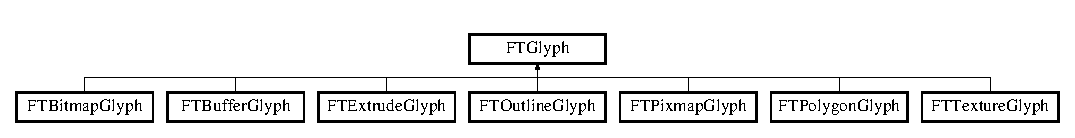
\includegraphics[height=1.403509cm]{classFTGlyph}
\end{center}
\end{figure}
\subsection*{Public Member Functions}
\begin{DoxyCompactItemize}
\item 
virtual {\bf $\sim$FTGlyph} ()
\begin{DoxyCompactList}\small\item\em Destructor. \item\end{DoxyCompactList}\item 
virtual const {\bf FTPoint} \& {\bf Render} (const {\bf FTPoint} \&pen, int renderMode)=0
\begin{DoxyCompactList}\small\item\em Renders this glyph at the current pen position. \item\end{DoxyCompactList}\item 
virtual float {\bf Advance} () const 
\begin{DoxyCompactList}\small\item\em Return the advance width for this glyph. \item\end{DoxyCompactList}\item 
virtual const {\bf FTBBox} \& {\bf BBox} () const 
\begin{DoxyCompactList}\small\item\em Return the bounding box for this glyph. \item\end{DoxyCompactList}\item 
virtual FT\_\-Error {\bf Error} () const 
\begin{DoxyCompactList}\small\item\em Queries for errors. \item\end{DoxyCompactList}\end{DoxyCompactItemize}
\subsection*{Protected Member Functions}
\begin{DoxyCompactItemize}
\item 
{\bf FTGlyph} (FT\_\-GlyphSlot glyph)
\begin{DoxyCompactList}\small\item\em Create a glyph. \item\end{DoxyCompactList}\end{DoxyCompactItemize}
\subsection*{Friends}
\begin{DoxyCompactItemize}
\item 
class {\bf FTBitmapGlyph}
\item 
class {\bf FTBufferGlyph}
\item 
class {\bf FTExtrudeGlyph}
\item 
class {\bf FTOutlineGlyph}
\item 
class {\bf FTPixmapGlyph}
\item 
class {\bf FTPolygonGlyph}
\item 
class {\bf FTTextureGlyph}
\end{DoxyCompactItemize}


\subsection{Detailed Description}
\doxyref{FTGlyph}{p.}{classFTGlyph} is the base class for \doxyref{FTGL}{p.}{namespaceFTGL} glyphs. It provides the interface between Freetype glyphs and their openGL renderable counterparts. This is an abstract class and derived classes must implement the {\ttfamily Render} function.

\begin{DoxySeeAlso}{See also}
\doxyref{FTBBox}{p.}{classFTBBox} 

\doxyref{FTPoint}{p.}{classFTPoint} 
\end{DoxySeeAlso}


Definition at line 50 of file FTGlyph.h.



\subsection{Constructor \& Destructor Documentation}
\index{FTGlyph@{FTGlyph}!FTGlyph@{FTGlyph}}
\index{FTGlyph@{FTGlyph}!FTGlyph@{FTGlyph}}
\subsubsection[{FTGlyph}]{\setlength{\rightskip}{0pt plus 5cm}FTGlyph::FTGlyph (
\begin{DoxyParamCaption}
\item[{FT\_\-GlyphSlot}]{ glyph}
\end{DoxyParamCaption}
)\hspace{0.3cm}{\ttfamily  [protected]}}\label{classFTGlyph_a4673d2a5da6ab44bcc0f2eb3326c30e8}


Create a glyph. 


\begin{DoxyParams}{Parameters}
{\em glyph} & The Freetype glyph to be processed \\
\hline
\end{DoxyParams}
\index{FTGlyph@{FTGlyph}!$\sim$FTGlyph@{$\sim$FTGlyph}}
\index{$\sim$FTGlyph@{$\sim$FTGlyph}!FTGlyph@{FTGlyph}}
\subsubsection[{$\sim$FTGlyph}]{\setlength{\rightskip}{0pt plus 5cm}virtual FTGlyph::$\sim$FTGlyph (
\begin{DoxyParamCaption}
{}
\end{DoxyParamCaption}
)\hspace{0.3cm}{\ttfamily  [virtual]}}\label{classFTGlyph_ad93a5124ddd9fe408e07f5054ab92452}


Destructor. 



\subsection{Member Function Documentation}
\index{FTGlyph@{FTGlyph}!Advance@{Advance}}
\index{Advance@{Advance}!FTGlyph@{FTGlyph}}
\subsubsection[{Advance}]{\setlength{\rightskip}{0pt plus 5cm}virtual float FTGlyph::Advance (
\begin{DoxyParamCaption}
{}
\end{DoxyParamCaption}
) const\hspace{0.3cm}{\ttfamily  [virtual]}}\label{classFTGlyph_a42fdc90fefe9d5550aca4339f88fbc5f}


Return the advance width for this glyph. 

\begin{DoxyReturn}{Returns}
advance width. 
\end{DoxyReturn}
\index{FTGlyph@{FTGlyph}!BBox@{BBox}}
\index{BBox@{BBox}!FTGlyph@{FTGlyph}}
\subsubsection[{BBox}]{\setlength{\rightskip}{0pt plus 5cm}virtual const {\bf FTBBox}\& FTGlyph::BBox (
\begin{DoxyParamCaption}
{}
\end{DoxyParamCaption}
) const\hspace{0.3cm}{\ttfamily  [virtual]}}\label{classFTGlyph_aa165c4c7de25de0a989753f56a3bc252}


Return the bounding box for this glyph. 

\begin{DoxyReturn}{Returns}
bounding box. 
\end{DoxyReturn}
\index{FTGlyph@{FTGlyph}!Error@{Error}}
\index{Error@{Error}!FTGlyph@{FTGlyph}}
\subsubsection[{Error}]{\setlength{\rightskip}{0pt plus 5cm}virtual FT\_\-Error FTGlyph::Error (
\begin{DoxyParamCaption}
{}
\end{DoxyParamCaption}
) const\hspace{0.3cm}{\ttfamily  [virtual]}}\label{classFTGlyph_a14fd6a0dc8b6e0e04a769e2e239b104b}


Queries for errors. 

\begin{DoxyReturn}{Returns}
The current error code. 
\end{DoxyReturn}
\index{FTGlyph@{FTGlyph}!Render@{Render}}
\index{Render@{Render}!FTGlyph@{FTGlyph}}
\subsubsection[{Render}]{\setlength{\rightskip}{0pt plus 5cm}virtual const {\bf FTPoint}\& FTGlyph::Render (
\begin{DoxyParamCaption}
\item[{const {\bf FTPoint} \&}]{ pen, }
\item[{int}]{ renderMode}
\end{DoxyParamCaption}
)\hspace{0.3cm}{\ttfamily  [pure virtual]}}\label{classFTGlyph_abcf3aef56d4bf022f6d95d5e287800df}


Renders this glyph at the current pen position. 


\begin{DoxyParams}{Parameters}
{\em pen} & The current pen position. \\
\hline
{\em renderMode} & Render mode to display \\
\hline
\end{DoxyParams}
\begin{DoxyReturn}{Returns}
The advance distance for this glyph. 
\end{DoxyReturn}


Implemented in {\bf FTBitmapGlyph} \doxyref{}{p.}{classFTBitmapGlyph_a7286040897f117da9f52023da795de42}, {\bf FTBufferGlyph} \doxyref{}{p.}{classFTBufferGlyph_a33bc5176b9c5739f20d634eca04a45a5}, {\bf FTExtrudeGlyph} \doxyref{}{p.}{classFTExtrudeGlyph_a48cc5da5e2e6491d79bcee8a9107bc60}, {\bf FTOutlineGlyph} \doxyref{}{p.}{classFTOutlineGlyph_ac0fcbe2023f8e8127144ad6a04627519}, {\bf FTPixmapGlyph} \doxyref{}{p.}{classFTPixmapGlyph_ac18ec8c2864d45d805e4fac5a980cddd}, {\bf FTPolygonGlyph} \doxyref{}{p.}{classFTPolygonGlyph_ae790f0d5d4d85bafb7c63edf537255b7}, and {\bf FTTextureGlyph} \doxyref{}{p.}{classFTTextureGlyph_a23d91684651a5cc913e6232c60dc58f4}.



\subsection{Friends And Related Function Documentation}
\index{FTGlyph@{FTGlyph}!FTBitmapGlyph@{FTBitmapGlyph}}
\index{FTBitmapGlyph@{FTBitmapGlyph}!FTGlyph@{FTGlyph}}
\subsubsection[{FTBitmapGlyph}]{\setlength{\rightskip}{0pt plus 5cm}friend class {\bf FTBitmapGlyph}\hspace{0.3cm}{\ttfamily  [friend]}}\label{classFTGlyph_aa3f0c28a7cfbfa0e896973476f7ed49d}


Definition at line 70 of file FTGlyph.h.

\index{FTGlyph@{FTGlyph}!FTBufferGlyph@{FTBufferGlyph}}
\index{FTBufferGlyph@{FTBufferGlyph}!FTGlyph@{FTGlyph}}
\subsubsection[{FTBufferGlyph}]{\setlength{\rightskip}{0pt plus 5cm}friend class {\bf FTBufferGlyph}\hspace{0.3cm}{\ttfamily  [friend]}}\label{classFTGlyph_a385e2288042fd77f037a715e7801b451}


Definition at line 71 of file FTGlyph.h.

\index{FTGlyph@{FTGlyph}!FTExtrudeGlyph@{FTExtrudeGlyph}}
\index{FTExtrudeGlyph@{FTExtrudeGlyph}!FTGlyph@{FTGlyph}}
\subsubsection[{FTExtrudeGlyph}]{\setlength{\rightskip}{0pt plus 5cm}friend class {\bf FTExtrudeGlyph}\hspace{0.3cm}{\ttfamily  [friend]}}\label{classFTGlyph_a43bdcab05c1db93d9474fee8176c1fb0}


Definition at line 72 of file FTGlyph.h.

\index{FTGlyph@{FTGlyph}!FTOutlineGlyph@{FTOutlineGlyph}}
\index{FTOutlineGlyph@{FTOutlineGlyph}!FTGlyph@{FTGlyph}}
\subsubsection[{FTOutlineGlyph}]{\setlength{\rightskip}{0pt plus 5cm}friend class {\bf FTOutlineGlyph}\hspace{0.3cm}{\ttfamily  [friend]}}\label{classFTGlyph_accb6ff0274a52a67e706edda49d6a201}


Definition at line 73 of file FTGlyph.h.

\index{FTGlyph@{FTGlyph}!FTPixmapGlyph@{FTPixmapGlyph}}
\index{FTPixmapGlyph@{FTPixmapGlyph}!FTGlyph@{FTGlyph}}
\subsubsection[{FTPixmapGlyph}]{\setlength{\rightskip}{0pt plus 5cm}friend class {\bf FTPixmapGlyph}\hspace{0.3cm}{\ttfamily  [friend]}}\label{classFTGlyph_ab141fccf761e39b9e4bec64cda0507a7}


Definition at line 74 of file FTGlyph.h.

\index{FTGlyph@{FTGlyph}!FTPolygonGlyph@{FTPolygonGlyph}}
\index{FTPolygonGlyph@{FTPolygonGlyph}!FTGlyph@{FTGlyph}}
\subsubsection[{FTPolygonGlyph}]{\setlength{\rightskip}{0pt plus 5cm}friend class {\bf FTPolygonGlyph}\hspace{0.3cm}{\ttfamily  [friend]}}\label{classFTGlyph_a0e33f7bc34e1097f8f9adcb6252d1bc0}


Definition at line 75 of file FTGlyph.h.

\index{FTGlyph@{FTGlyph}!FTTextureGlyph@{FTTextureGlyph}}
\index{FTTextureGlyph@{FTTextureGlyph}!FTGlyph@{FTGlyph}}
\subsubsection[{FTTextureGlyph}]{\setlength{\rightskip}{0pt plus 5cm}friend class {\bf FTTextureGlyph}\hspace{0.3cm}{\ttfamily  [friend]}}\label{classFTGlyph_a01c2ee1e01ccd33e4f1f26f2478a74a0}


Definition at line 76 of file FTGlyph.h.



The documentation for this class was generated from the following file:\begin{DoxyCompactItemize}
\item 
{\bf FTGlyph.h}\end{DoxyCompactItemize}

\section{FTLayout Class Reference}
\label{classFTLayout}\index{FTLayout@{FTLayout}}


\doxyref{FTLayout}{p.}{classFTLayout} is the interface for layout managers that render text.  




{\ttfamily \#include $<$FTLayout.h$>$}

Inheritance diagram for FTLayout:\begin{figure}[H]
\begin{center}
\leavevmode
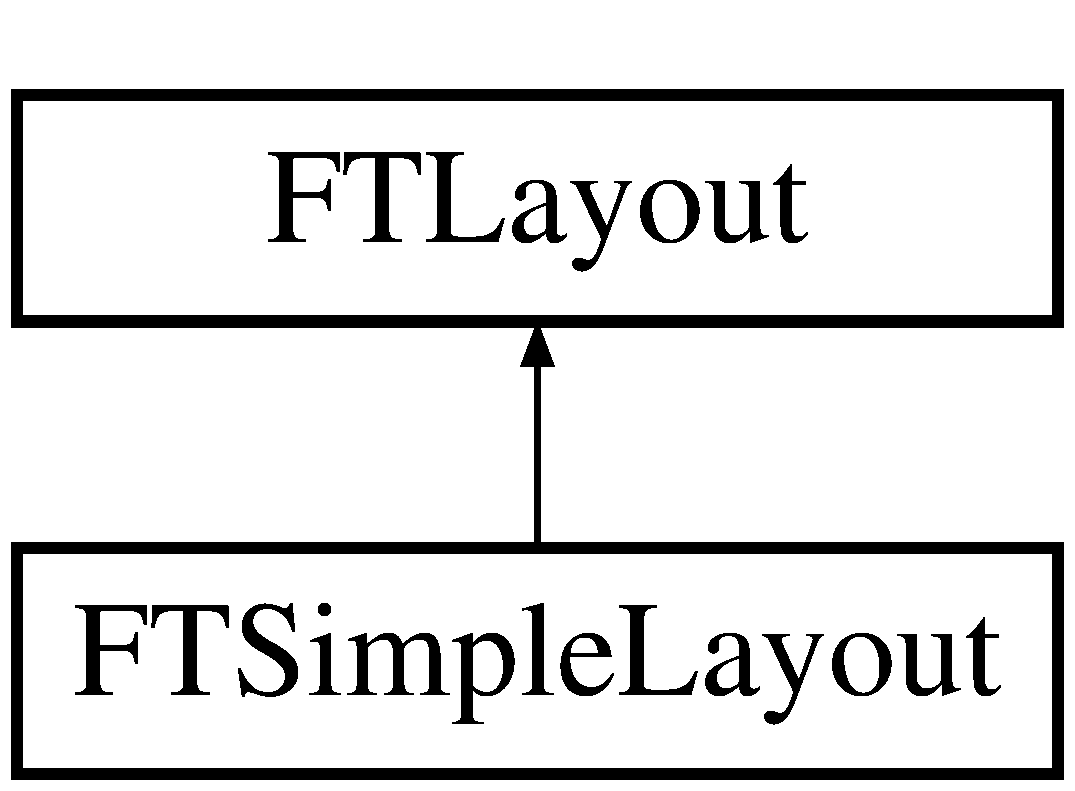
\includegraphics[height=2.000000cm]{classFTLayout}
\end{center}
\end{figure}
\subsection*{Public Member Functions}
\begin{DoxyCompactItemize}
\item 
virtual {\bf $\sim$FTLayout} ()
\begin{DoxyCompactList}\small\item\em Destructor. \item\end{DoxyCompactList}\item 
virtual {\bf FTBBox} {\bf BBox} (const char $\ast$string, const int len=-\/1, {\bf FTPoint} position={\bf FTPoint}())=0
\begin{DoxyCompactList}\small\item\em Get the bounding box for a formatted string. \item\end{DoxyCompactList}\item 
virtual {\bf FTBBox} {\bf BBox} (const wchar\_\-t $\ast$string, const int len=-\/1, {\bf FTPoint} position={\bf FTPoint}())=0
\begin{DoxyCompactList}\small\item\em Get the bounding box for a formatted string. \item\end{DoxyCompactList}\item 
virtual void {\bf Render} (const char $\ast$string, const int len=-\/1, {\bf FTPoint} position={\bf FTPoint}(), int renderMode=FTGL::RENDER\_\-ALL)=0
\begin{DoxyCompactList}\small\item\em Render a string of characters. \item\end{DoxyCompactList}\item 
virtual void {\bf Render} (const wchar\_\-t $\ast$string, const int len=-\/1, {\bf FTPoint} position={\bf FTPoint}(), int renderMode=FTGL::RENDER\_\-ALL)=0
\begin{DoxyCompactList}\small\item\em Render a string of characters. \item\end{DoxyCompactList}\item 
virtual FT\_\-Error {\bf Error} () const 
\begin{DoxyCompactList}\small\item\em Queries the Layout for errors. \item\end{DoxyCompactList}\end{DoxyCompactItemize}
\subsection*{Protected Member Functions}
\begin{DoxyCompactItemize}
\item 
{\bf FTLayout} ()
\end{DoxyCompactItemize}
\subsection*{Friends}
\begin{DoxyCompactItemize}
\item 
class {\bf FTSimpleLayout}
\end{DoxyCompactItemize}


\subsection{Detailed Description}
\doxyref{FTLayout}{p.}{classFTLayout} is the interface for layout managers that render text. Specific layout manager classes are derived from this class. This class is abstract and deriving classes must implement the protected {\ttfamily Render} methods to render formatted text and {\ttfamily BBox} methods to determine the bounding box of output text.

\begin{DoxySeeAlso}{See also}
\doxyref{FTFont}{p.}{classFTFont} 

\doxyref{FTBBox}{p.}{classFTBBox} 
\end{DoxySeeAlso}


Definition at line 52 of file FTLayout.h.



\subsection{Constructor \& Destructor Documentation}
\index{FTLayout@{FTLayout}!FTLayout@{FTLayout}}
\index{FTLayout@{FTLayout}!FTLayout@{FTLayout}}
\subsubsection[{FTLayout}]{\setlength{\rightskip}{0pt plus 5cm}FTLayout::FTLayout (
\begin{DoxyParamCaption}
{}
\end{DoxyParamCaption}
)\hspace{0.3cm}{\ttfamily  [protected]}}\label{classFTLayout_a7b51099482c3f3171337915d42c9cd2b}
\index{FTLayout@{FTLayout}!$\sim$FTLayout@{$\sim$FTLayout}}
\index{$\sim$FTLayout@{$\sim$FTLayout}!FTLayout@{FTLayout}}
\subsubsection[{$\sim$FTLayout}]{\setlength{\rightskip}{0pt plus 5cm}virtual FTLayout::$\sim$FTLayout (
\begin{DoxyParamCaption}
{}
\end{DoxyParamCaption}
)\hspace{0.3cm}{\ttfamily  [virtual]}}\label{classFTLayout_aee0787f8975a809261fb49813f0baac4}


Destructor. 



\subsection{Member Function Documentation}
\index{FTLayout@{FTLayout}!BBox@{BBox}}
\index{BBox@{BBox}!FTLayout@{FTLayout}}
\subsubsection[{BBox}]{\setlength{\rightskip}{0pt plus 5cm}virtual {\bf FTBBox} FTLayout::BBox (
\begin{DoxyParamCaption}
\item[{const char $\ast$}]{ string, }
\item[{const int}]{ len = {\ttfamily -\/1}, }
\item[{{\bf FTPoint}}]{ position = {\ttfamily {\bf FTPoint}()}}
\end{DoxyParamCaption}
)\hspace{0.3cm}{\ttfamily  [pure virtual]}}\label{classFTLayout_ae79561f22ee39e69ce27d84b1d47fe2e}


Get the bounding box for a formatted string. 


\begin{DoxyParams}{Parameters}
{\em string} & A char string. \\
\hline
{\em len} & The length of the string. If $<$ 0 then all characters will be checked until a null character is encountered (optional). \\
\hline
{\em position} & The pen position of the first character (optional). \\
\hline
\end{DoxyParams}
\begin{DoxyReturn}{Returns}
The corresponding bounding box. 
\end{DoxyReturn}


Implemented in {\bf FTSimpleLayout} \doxyref{}{p.}{classFTSimpleLayout_a132c938c66912fe0b2360152349f887c}.

\index{FTLayout@{FTLayout}!BBox@{BBox}}
\index{BBox@{BBox}!FTLayout@{FTLayout}}
\subsubsection[{BBox}]{\setlength{\rightskip}{0pt plus 5cm}virtual {\bf FTBBox} FTLayout::BBox (
\begin{DoxyParamCaption}
\item[{const wchar\_\-t $\ast$}]{ string, }
\item[{const int}]{ len = {\ttfamily -\/1}, }
\item[{{\bf FTPoint}}]{ position = {\ttfamily {\bf FTPoint}()}}
\end{DoxyParamCaption}
)\hspace{0.3cm}{\ttfamily  [pure virtual]}}\label{classFTLayout_abf64582771a2281d901af1e074535c2a}


Get the bounding box for a formatted string. 


\begin{DoxyParams}{Parameters}
{\em string} & A wchar\_\-t string. \\
\hline
{\em len} & The length of the string. If $<$ 0 then all characters will be checked until a null character is encountered (optional). \\
\hline
{\em position} & The pen position of the first character (optional). \\
\hline
\end{DoxyParams}
\begin{DoxyReturn}{Returns}
The corresponding bounding box. 
\end{DoxyReturn}


Implemented in {\bf FTSimpleLayout} \doxyref{}{p.}{classFTSimpleLayout_afdec41319af9fbeec0316e38d0661107}.

\index{FTLayout@{FTLayout}!Error@{Error}}
\index{Error@{Error}!FTLayout@{FTLayout}}
\subsubsection[{Error}]{\setlength{\rightskip}{0pt plus 5cm}virtual FT\_\-Error FTLayout::Error (
\begin{DoxyParamCaption}
{}
\end{DoxyParamCaption}
) const\hspace{0.3cm}{\ttfamily  [virtual]}}\label{classFTLayout_a83cf3e7565bf9d9d2aec6d0614d1e6fc}


Queries the Layout for errors. 

\begin{DoxyReturn}{Returns}
The current error code. 
\end{DoxyReturn}
\index{FTLayout@{FTLayout}!Render@{Render}}
\index{Render@{Render}!FTLayout@{FTLayout}}
\subsubsection[{Render}]{\setlength{\rightskip}{0pt plus 5cm}virtual void FTLayout::Render (
\begin{DoxyParamCaption}
\item[{const char $\ast$}]{ string, }
\item[{const int}]{ len = {\ttfamily -\/1}, }
\item[{{\bf FTPoint}}]{ position = {\ttfamily {\bf FTPoint}()}, }
\item[{int}]{ renderMode = {\ttfamily FTGL::RENDER\_\-ALL}}
\end{DoxyParamCaption}
)\hspace{0.3cm}{\ttfamily  [pure virtual]}}\label{classFTLayout_a0e18bf877bbfe871e93ec0ebf1437a0f}


Render a string of characters. 


\begin{DoxyParams}{Parameters}
{\em string} & 'C' style string to be output. \\
\hline
{\em len} & The length of the string. If $<$ 0 then all characters will be displayed until a null character is encountered (optional). \\
\hline
{\em position} & The pen position of the first character (optional). \\
\hline
{\em renderMode} & Render mode to display (optional) \\
\hline
\end{DoxyParams}


Implemented in {\bf FTSimpleLayout} \doxyref{}{p.}{classFTSimpleLayout_afc122918b71e571155ca714eeb5c4888}.

\index{FTLayout@{FTLayout}!Render@{Render}}
\index{Render@{Render}!FTLayout@{FTLayout}}
\subsubsection[{Render}]{\setlength{\rightskip}{0pt plus 5cm}virtual void FTLayout::Render (
\begin{DoxyParamCaption}
\item[{const wchar\_\-t $\ast$}]{ string, }
\item[{const int}]{ len = {\ttfamily -\/1}, }
\item[{{\bf FTPoint}}]{ position = {\ttfamily {\bf FTPoint}()}, }
\item[{int}]{ renderMode = {\ttfamily FTGL::RENDER\_\-ALL}}
\end{DoxyParamCaption}
)\hspace{0.3cm}{\ttfamily  [pure virtual]}}\label{classFTLayout_a793a7b371c885420d73acc56a667d53a}


Render a string of characters. 


\begin{DoxyParams}{Parameters}
{\em string} & wchar\_\-t string to be output. \\
\hline
{\em len} & The length of the string. If $<$ 0 then all characters will be displayed until a null character is encountered (optional). \\
\hline
{\em position} & The pen position of the first character (optional). \\
\hline
{\em renderMode} & Render mode to display (optional) \\
\hline
\end{DoxyParams}


Implemented in {\bf FTSimpleLayout} \doxyref{}{p.}{classFTSimpleLayout_aeea681385258bf9cd20c355555c9dbaf}.



\subsection{Friends And Related Function Documentation}
\index{FTLayout@{FTLayout}!FTSimpleLayout@{FTSimpleLayout}}
\index{FTSimpleLayout@{FTSimpleLayout}!FTLayout@{FTLayout}}
\subsubsection[{FTSimpleLayout}]{\setlength{\rightskip}{0pt plus 5cm}friend class {\bf FTSimpleLayout}\hspace{0.3cm}{\ttfamily  [friend]}}\label{classFTLayout_ae27eaa779922d14c8eb0f476456c7099}


Definition at line 67 of file FTLayout.h.



The documentation for this class was generated from the following file:\begin{DoxyCompactItemize}
\item 
{\bf FTLayout.h}\end{DoxyCompactItemize}

\section{FTOutlineFont Class Reference}
\label{classFTOutlineFont}\index{FTOutlineFont@{FTOutlineFont}}


\doxyref{FTOutlineFont}{p.}{classFTOutlineFont} is a specialisation of the \doxyref{FTFont}{p.}{classFTFont} class for handling Vector Outline fonts.  




{\ttfamily \#include $<$FTGLOutlineFont.h$>$}

Inheritance diagram for FTOutlineFont:\begin{figure}[H]
\begin{center}
\leavevmode
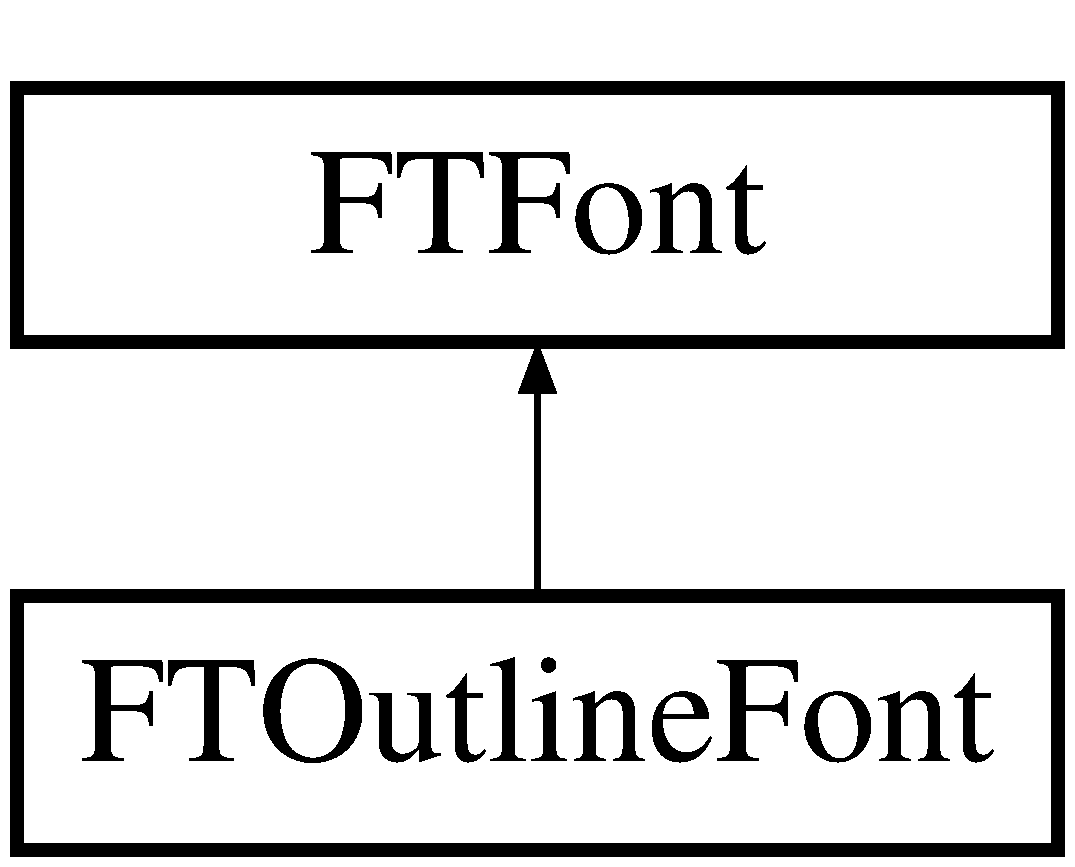
\includegraphics[height=2.000000cm]{classFTOutlineFont}
\end{center}
\end{figure}
\subsection*{Public Member Functions}
\begin{DoxyCompactItemize}
\item 
{\bf FTOutlineFont} (const char $\ast$fontFilePath)
\begin{DoxyCompactList}\small\item\em Open and read a font file. \item\end{DoxyCompactList}\item 
{\bf FTOutlineFont} (const unsigned char $\ast$pBufferBytes, size\_\-t bufferSizeInBytes)
\begin{DoxyCompactList}\small\item\em Open and read a font from a buffer in memory. \item\end{DoxyCompactList}\item 
{\bf $\sim$FTOutlineFont} ()
\begin{DoxyCompactList}\small\item\em Destructor. \item\end{DoxyCompactList}\end{DoxyCompactItemize}
\subsection*{Protected Member Functions}
\begin{DoxyCompactItemize}
\item 
virtual {\bf FTGlyph} $\ast$ {\bf MakeGlyph} (FT\_\-GlyphSlot slot)
\begin{DoxyCompactList}\small\item\em Construct a glyph of the correct type. \item\end{DoxyCompactList}\end{DoxyCompactItemize}


\subsection{Detailed Description}
\doxyref{FTOutlineFont}{p.}{classFTOutlineFont} is a specialisation of the \doxyref{FTFont}{p.}{classFTFont} class for handling Vector Outline fonts. \begin{DoxySeeAlso}{See also}
\doxyref{FTFont}{p.}{classFTFont} 
\end{DoxySeeAlso}


Definition at line 45 of file FTGLOutlineFont.h.



\subsection{Constructor \& Destructor Documentation}
\index{FTOutlineFont@{FTOutlineFont}!FTOutlineFont@{FTOutlineFont}}
\index{FTOutlineFont@{FTOutlineFont}!FTOutlineFont@{FTOutlineFont}}
\subsubsection[{FTOutlineFont}]{\setlength{\rightskip}{0pt plus 5cm}FTOutlineFont::FTOutlineFont (
\begin{DoxyParamCaption}
\item[{const char $\ast$}]{ fontFilePath}
\end{DoxyParamCaption}
)}\label{classFTOutlineFont_a248f6a8fa1244c7bff53f1c799c8163f}


Open and read a font file. 

Sets Error flag.


\begin{DoxyParams}{Parameters}
{\em fontFilePath} & font file path. \\
\hline
\end{DoxyParams}
\index{FTOutlineFont@{FTOutlineFont}!FTOutlineFont@{FTOutlineFont}}
\index{FTOutlineFont@{FTOutlineFont}!FTOutlineFont@{FTOutlineFont}}
\subsubsection[{FTOutlineFont}]{\setlength{\rightskip}{0pt plus 5cm}FTOutlineFont::FTOutlineFont (
\begin{DoxyParamCaption}
\item[{const unsigned char $\ast$}]{ pBufferBytes, }
\item[{size\_\-t}]{ bufferSizeInBytes}
\end{DoxyParamCaption}
)}\label{classFTOutlineFont_a6618bdb1b3a672d4d6750627cf1dac0c}


Open and read a font from a buffer in memory. 

Sets Error flag. The buffer is owned by the client and is NOT copied by \doxyref{FTGL}{p.}{namespaceFTGL}. The pointer must be valid while using \doxyref{FTGL}{p.}{namespaceFTGL}.


\begin{DoxyParams}{Parameters}
{\em pBufferBytes} & the in-\/memory buffer \\
\hline
{\em bufferSizeInBytes} & the length of the buffer in bytes \\
\hline
\end{DoxyParams}
\index{FTOutlineFont@{FTOutlineFont}!$\sim$FTOutlineFont@{$\sim$FTOutlineFont}}
\index{$\sim$FTOutlineFont@{$\sim$FTOutlineFont}!FTOutlineFont@{FTOutlineFont}}
\subsubsection[{$\sim$FTOutlineFont}]{\setlength{\rightskip}{0pt plus 5cm}FTOutlineFont::$\sim$FTOutlineFont (
\begin{DoxyParamCaption}
{}
\end{DoxyParamCaption}
)}\label{classFTOutlineFont_a2ac40cf9e9013fc2e82b98a55e0fa28e}


Destructor. 



\subsection{Member Function Documentation}
\index{FTOutlineFont@{FTOutlineFont}!MakeGlyph@{MakeGlyph}}
\index{MakeGlyph@{MakeGlyph}!FTOutlineFont@{FTOutlineFont}}
\subsubsection[{MakeGlyph}]{\setlength{\rightskip}{0pt plus 5cm}virtual {\bf FTGlyph}$\ast$ FTOutlineFont::MakeGlyph (
\begin{DoxyParamCaption}
\item[{FT\_\-GlyphSlot}]{ slot}
\end{DoxyParamCaption}
)\hspace{0.3cm}{\ttfamily  [protected, virtual]}}\label{classFTOutlineFont_a39df452446d15bd1d78ede61ae3f8c27}


Construct a glyph of the correct type. 

Clients must override the function and return their specialised \doxyref{FTGlyph}{p.}{classFTGlyph}.


\begin{DoxyParams}{Parameters}
{\em slot} & A FreeType glyph slot. \\
\hline
\end{DoxyParams}
\begin{DoxyReturn}{Returns}
An FT$\ast$$\ast$$\ast$$\ast$Glyph or {\ttfamily null} on failure. 
\end{DoxyReturn}


Implements {\bf FTFont} \doxyref{}{p.}{classFTFont_a07f8bef6c3bd52e7d905e6db17c9b8e6}.



The documentation for this class was generated from the following file:\begin{DoxyCompactItemize}
\item 
{\bf FTGLOutlineFont.h}\end{DoxyCompactItemize}

\section{FTOutlineGlyph Class Reference}
\label{classFTOutlineGlyph}\index{FTOutlineGlyph@{FTOutlineGlyph}}


\doxyref{FTOutlineGlyph}{p.}{classFTOutlineGlyph} is a specialisation of \doxyref{FTGlyph}{p.}{classFTGlyph} for creating outlines.  




{\ttfamily \#include $<$FTOutlineGlyph.h$>$}

Inheritance diagram for FTOutlineGlyph:\begin{figure}[H]
\begin{center}
\leavevmode
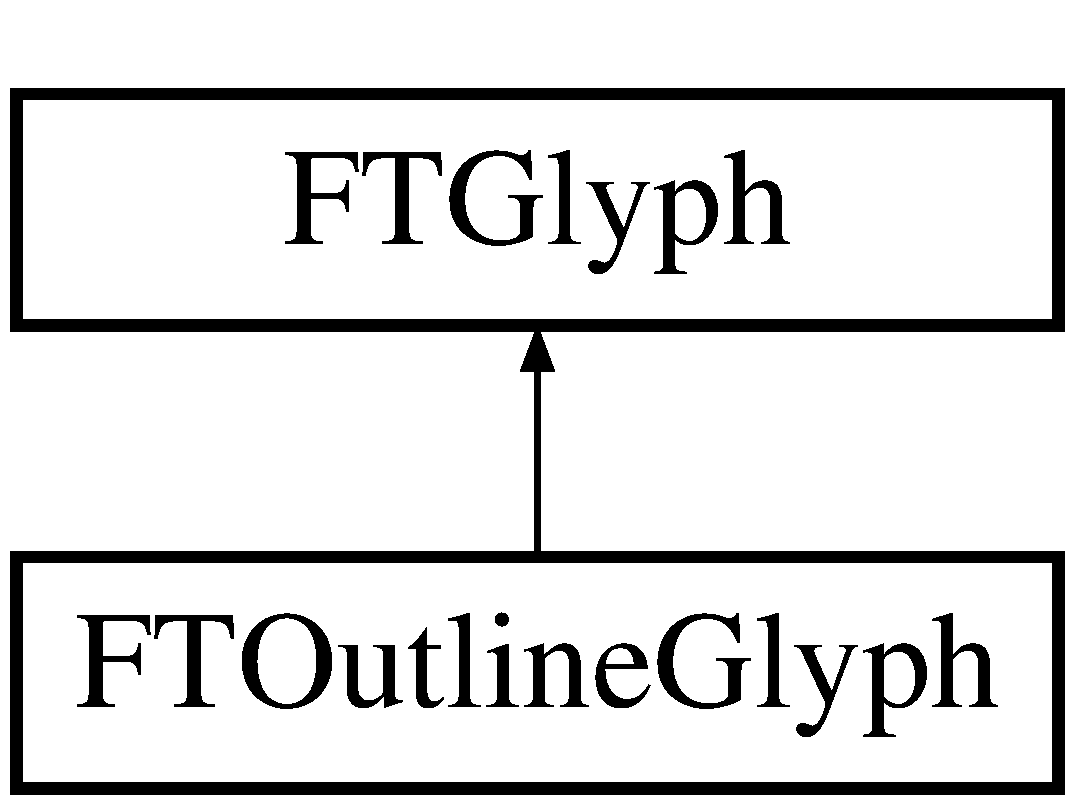
\includegraphics[height=2.000000cm]{classFTOutlineGlyph}
\end{center}
\end{figure}
\subsection*{Public Member Functions}
\begin{DoxyCompactItemize}
\item 
{\bf FTOutlineGlyph} (FT\_\-GlyphSlot glyph, float outset, bool useDisplayList)
\begin{DoxyCompactList}\small\item\em Constructor. \item\end{DoxyCompactList}\item 
virtual {\bf $\sim$FTOutlineGlyph} ()
\begin{DoxyCompactList}\small\item\em Destructor. \item\end{DoxyCompactList}\item 
virtual const {\bf FTPoint} \& {\bf Render} (const {\bf FTPoint} \&pen, int renderMode)
\begin{DoxyCompactList}\small\item\em Render this glyph at the current pen position. \item\end{DoxyCompactList}\end{DoxyCompactItemize}


\subsection{Detailed Description}
\doxyref{FTOutlineGlyph}{p.}{classFTOutlineGlyph} is a specialisation of \doxyref{FTGlyph}{p.}{classFTGlyph} for creating outlines. 

Definition at line 42 of file FTOutlineGlyph.h.



\subsection{Constructor \& Destructor Documentation}
\index{FTOutlineGlyph@{FTOutlineGlyph}!FTOutlineGlyph@{FTOutlineGlyph}}
\index{FTOutlineGlyph@{FTOutlineGlyph}!FTOutlineGlyph@{FTOutlineGlyph}}
\subsubsection[{FTOutlineGlyph}]{\setlength{\rightskip}{0pt plus 5cm}FTOutlineGlyph::FTOutlineGlyph (
\begin{DoxyParamCaption}
\item[{FT\_\-GlyphSlot}]{ glyph, }
\item[{float}]{ outset, }
\item[{bool}]{ useDisplayList}
\end{DoxyParamCaption}
)}\label{classFTOutlineGlyph_a4a45e11e8e1fca206ed808a433389c83}


Constructor. 

Sets the Error to Invalid\_\-Outline if the glyphs isn't an outline.


\begin{DoxyParams}{Parameters}
{\em glyph} & The Freetype glyph to be processed \\
\hline
{\em outset} & outset distance \\
\hline
{\em useDisplayList} & Enable or disable the use of Display Lists for this glyph {\ttfamily true} turns ON display lists. {\ttfamily false} turns OFF display lists. \\
\hline
\end{DoxyParams}
\index{FTOutlineGlyph@{FTOutlineGlyph}!$\sim$FTOutlineGlyph@{$\sim$FTOutlineGlyph}}
\index{$\sim$FTOutlineGlyph@{$\sim$FTOutlineGlyph}!FTOutlineGlyph@{FTOutlineGlyph}}
\subsubsection[{$\sim$FTOutlineGlyph}]{\setlength{\rightskip}{0pt plus 5cm}virtual FTOutlineGlyph::$\sim$FTOutlineGlyph (
\begin{DoxyParamCaption}
{}
\end{DoxyParamCaption}
)\hspace{0.3cm}{\ttfamily  [virtual]}}\label{classFTOutlineGlyph_aacf6d78d4335864d96e07142e540e150}


Destructor. 



\subsection{Member Function Documentation}
\index{FTOutlineGlyph@{FTOutlineGlyph}!Render@{Render}}
\index{Render@{Render}!FTOutlineGlyph@{FTOutlineGlyph}}
\subsubsection[{Render}]{\setlength{\rightskip}{0pt plus 5cm}virtual const {\bf FTPoint}\& FTOutlineGlyph::Render (
\begin{DoxyParamCaption}
\item[{const {\bf FTPoint} \&}]{ pen, }
\item[{int}]{ renderMode}
\end{DoxyParamCaption}
)\hspace{0.3cm}{\ttfamily  [virtual]}}\label{classFTOutlineGlyph_ac0fcbe2023f8e8127144ad6a04627519}


Render this glyph at the current pen position. 


\begin{DoxyParams}{Parameters}
{\em pen} & The current pen position. \\
\hline
{\em renderMode} & Render mode to display \\
\hline
\end{DoxyParams}
\begin{DoxyReturn}{Returns}
The advance distance for this glyph. 
\end{DoxyReturn}


Implements {\bf FTGlyph} \doxyref{}{p.}{classFTGlyph_abcf3aef56d4bf022f6d95d5e287800df}.



The documentation for this class was generated from the following file:\begin{DoxyCompactItemize}
\item 
{\bf FTOutlineGlyph.h}\end{DoxyCompactItemize}

\section{FTPixmapFont Class Reference}
\label{classFTPixmapFont}\index{FTPixmapFont@{FTPixmapFont}}


\doxyref{FTPixmapFont}{p.}{classFTPixmapFont} is a specialisation of the \doxyref{FTFont}{p.}{classFTFont} class for handling Pixmap (Grey Scale) fonts.  




{\ttfamily \#include $<$FTGLPixmapFont.h$>$}

Inheritance diagram for FTPixmapFont:\begin{figure}[H]
\begin{center}
\leavevmode
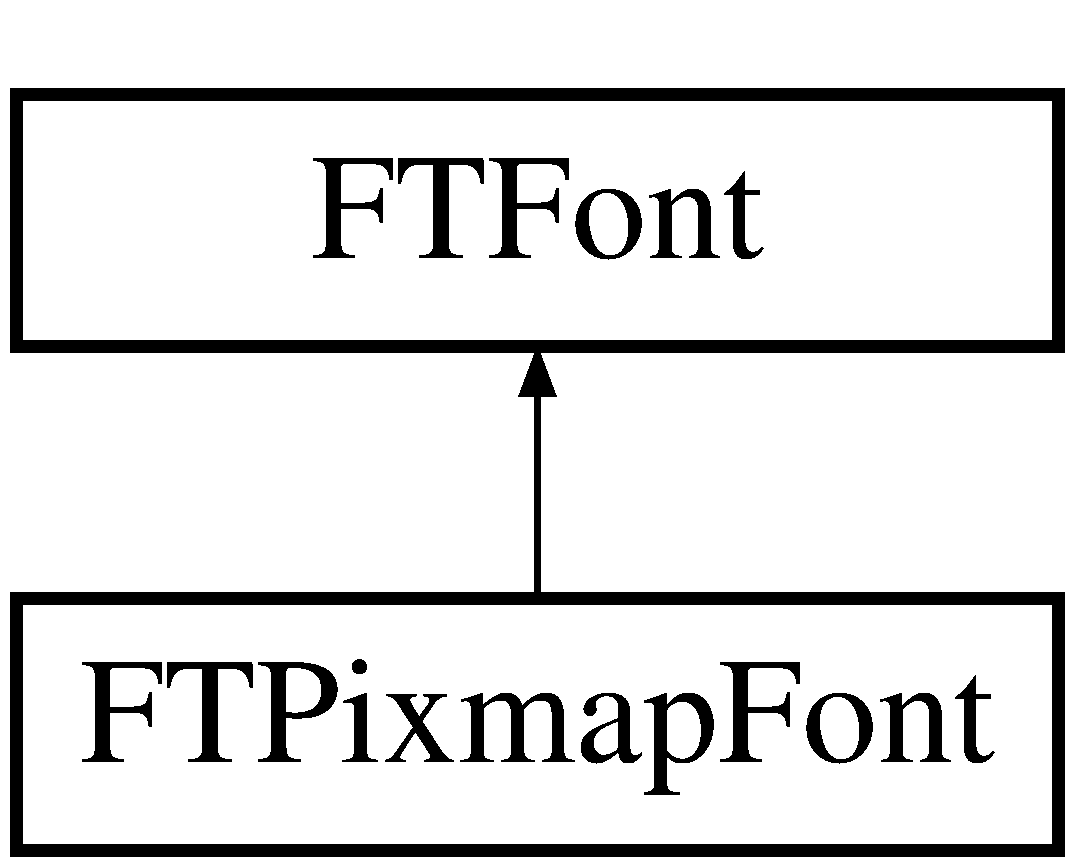
\includegraphics[height=2.000000cm]{classFTPixmapFont}
\end{center}
\end{figure}
\subsection*{Public Member Functions}
\begin{DoxyCompactItemize}
\item 
{\bf FTPixmapFont} (const char $\ast$fontFilePath)
\begin{DoxyCompactList}\small\item\em Open and read a font file. \item\end{DoxyCompactList}\item 
{\bf FTPixmapFont} (const unsigned char $\ast$pBufferBytes, size\_\-t bufferSizeInBytes)
\begin{DoxyCompactList}\small\item\em Open and read a font from a buffer in memory. \item\end{DoxyCompactList}\item 
{\bf $\sim$FTPixmapFont} ()
\begin{DoxyCompactList}\small\item\em Destructor. \item\end{DoxyCompactList}\end{DoxyCompactItemize}
\subsection*{Protected Member Functions}
\begin{DoxyCompactItemize}
\item 
virtual {\bf FTGlyph} $\ast$ {\bf MakeGlyph} (FT\_\-GlyphSlot slot)
\begin{DoxyCompactList}\small\item\em Construct a glyph of the correct type. \item\end{DoxyCompactList}\end{DoxyCompactItemize}


\subsection{Detailed Description}
\doxyref{FTPixmapFont}{p.}{classFTPixmapFont} is a specialisation of the \doxyref{FTFont}{p.}{classFTFont} class for handling Pixmap (Grey Scale) fonts. \begin{DoxySeeAlso}{See also}
\doxyref{FTFont}{p.}{classFTFont} 
\end{DoxySeeAlso}


Definition at line 45 of file FTGLPixmapFont.h.



\subsection{Constructor \& Destructor Documentation}
\index{FTPixmapFont@{FTPixmapFont}!FTPixmapFont@{FTPixmapFont}}
\index{FTPixmapFont@{FTPixmapFont}!FTPixmapFont@{FTPixmapFont}}
\subsubsection[{FTPixmapFont}]{\setlength{\rightskip}{0pt plus 5cm}FTPixmapFont::FTPixmapFont (
\begin{DoxyParamCaption}
\item[{const char $\ast$}]{ fontFilePath}
\end{DoxyParamCaption}
)}\label{classFTPixmapFont_a7059546858ab96667edbd017b3eb282f}


Open and read a font file. 

Sets Error flag.


\begin{DoxyParams}{Parameters}
{\em fontFilePath} & font file path. \\
\hline
\end{DoxyParams}
\index{FTPixmapFont@{FTPixmapFont}!FTPixmapFont@{FTPixmapFont}}
\index{FTPixmapFont@{FTPixmapFont}!FTPixmapFont@{FTPixmapFont}}
\subsubsection[{FTPixmapFont}]{\setlength{\rightskip}{0pt plus 5cm}FTPixmapFont::FTPixmapFont (
\begin{DoxyParamCaption}
\item[{const unsigned char $\ast$}]{ pBufferBytes, }
\item[{size\_\-t}]{ bufferSizeInBytes}
\end{DoxyParamCaption}
)}\label{classFTPixmapFont_ab901b6cd034c8a888e732a568d68cb5b}


Open and read a font from a buffer in memory. 

Sets Error flag. The buffer is owned by the client and is NOT copied by \doxyref{FTGL}{p.}{namespaceFTGL}. The pointer must be valid while using \doxyref{FTGL}{p.}{namespaceFTGL}.


\begin{DoxyParams}{Parameters}
{\em pBufferBytes} & the in-\/memory buffer \\
\hline
{\em bufferSizeInBytes} & the length of the buffer in bytes \\
\hline
\end{DoxyParams}
\index{FTPixmapFont@{FTPixmapFont}!$\sim$FTPixmapFont@{$\sim$FTPixmapFont}}
\index{$\sim$FTPixmapFont@{$\sim$FTPixmapFont}!FTPixmapFont@{FTPixmapFont}}
\subsubsection[{$\sim$FTPixmapFont}]{\setlength{\rightskip}{0pt plus 5cm}FTPixmapFont::$\sim$FTPixmapFont (
\begin{DoxyParamCaption}
{}
\end{DoxyParamCaption}
)}\label{classFTPixmapFont_afb29aeafcdbb9366c548ed9d0e80d88c}


Destructor. 



\subsection{Member Function Documentation}
\index{FTPixmapFont@{FTPixmapFont}!MakeGlyph@{MakeGlyph}}
\index{MakeGlyph@{MakeGlyph}!FTPixmapFont@{FTPixmapFont}}
\subsubsection[{MakeGlyph}]{\setlength{\rightskip}{0pt plus 5cm}virtual {\bf FTGlyph}$\ast$ FTPixmapFont::MakeGlyph (
\begin{DoxyParamCaption}
\item[{FT\_\-GlyphSlot}]{ slot}
\end{DoxyParamCaption}
)\hspace{0.3cm}{\ttfamily  [protected, virtual]}}\label{classFTPixmapFont_ad0c48c6be9dca736f6f37032a8a25d84}


Construct a glyph of the correct type. 

Clients must override the function and return their specialised \doxyref{FTGlyph}{p.}{classFTGlyph}.


\begin{DoxyParams}{Parameters}
{\em slot} & A FreeType glyph slot. \\
\hline
\end{DoxyParams}
\begin{DoxyReturn}{Returns}
An FT$\ast$$\ast$$\ast$$\ast$Glyph or {\ttfamily null} on failure. 
\end{DoxyReturn}


Implements {\bf FTFont} \doxyref{}{p.}{classFTFont_a07f8bef6c3bd52e7d905e6db17c9b8e6}.



The documentation for this class was generated from the following file:\begin{DoxyCompactItemize}
\item 
{\bf FTGLPixmapFont.h}\end{DoxyCompactItemize}

\section{FTPixmapGlyph Class Reference}
\label{classFTPixmapGlyph}\index{FTPixmapGlyph@{FTPixmapGlyph}}


\doxyref{FTPixmapGlyph}{p.}{classFTPixmapGlyph} is a specialisation of \doxyref{FTGlyph}{p.}{classFTGlyph} for creating pixmaps.  




{\ttfamily \#include $<$FTPixmapGlyph.h$>$}

Inheritance diagram for FTPixmapGlyph:\begin{figure}[H]
\begin{center}
\leavevmode
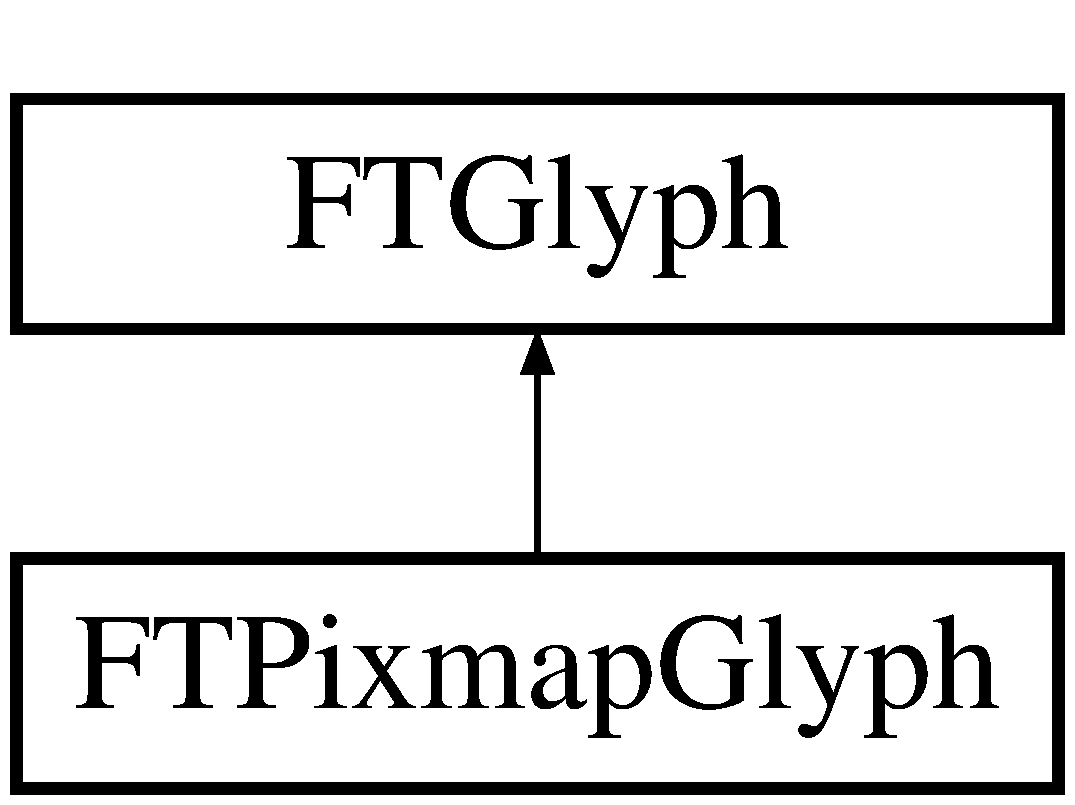
\includegraphics[height=2.000000cm]{classFTPixmapGlyph}
\end{center}
\end{figure}
\subsection*{Public Member Functions}
\begin{DoxyCompactItemize}
\item 
{\bf FTPixmapGlyph} (FT\_\-GlyphSlot glyph)
\begin{DoxyCompactList}\small\item\em Constructor. \item\end{DoxyCompactList}\item 
virtual {\bf $\sim$FTPixmapGlyph} ()
\begin{DoxyCompactList}\small\item\em Destructor. \item\end{DoxyCompactList}\item 
virtual const {\bf FTPoint} \& {\bf Render} (const {\bf FTPoint} \&pen, int renderMode)
\begin{DoxyCompactList}\small\item\em Render this glyph at the current pen position. \item\end{DoxyCompactList}\end{DoxyCompactItemize}


\subsection{Detailed Description}
\doxyref{FTPixmapGlyph}{p.}{classFTPixmapGlyph} is a specialisation of \doxyref{FTGlyph}{p.}{classFTGlyph} for creating pixmaps. 

Definition at line 42 of file FTPixmapGlyph.h.



\subsection{Constructor \& Destructor Documentation}
\index{FTPixmapGlyph@{FTPixmapGlyph}!FTPixmapGlyph@{FTPixmapGlyph}}
\index{FTPixmapGlyph@{FTPixmapGlyph}!FTPixmapGlyph@{FTPixmapGlyph}}
\subsubsection[{FTPixmapGlyph}]{\setlength{\rightskip}{0pt plus 5cm}FTPixmapGlyph::FTPixmapGlyph (
\begin{DoxyParamCaption}
\item[{FT\_\-GlyphSlot}]{ glyph}
\end{DoxyParamCaption}
)}\label{classFTPixmapGlyph_a3f3978f9c2a8fda401d0ce9ccc2ebb7d}


Constructor. 


\begin{DoxyParams}{Parameters}
{\em glyph} & The Freetype glyph to be processed \\
\hline
\end{DoxyParams}
\index{FTPixmapGlyph@{FTPixmapGlyph}!$\sim$FTPixmapGlyph@{$\sim$FTPixmapGlyph}}
\index{$\sim$FTPixmapGlyph@{$\sim$FTPixmapGlyph}!FTPixmapGlyph@{FTPixmapGlyph}}
\subsubsection[{$\sim$FTPixmapGlyph}]{\setlength{\rightskip}{0pt plus 5cm}virtual FTPixmapGlyph::$\sim$FTPixmapGlyph (
\begin{DoxyParamCaption}
{}
\end{DoxyParamCaption}
)\hspace{0.3cm}{\ttfamily  [virtual]}}\label{classFTPixmapGlyph_a4ff9f3d8e748fae9c9c1e704a0fbced5}


Destructor. 



\subsection{Member Function Documentation}
\index{FTPixmapGlyph@{FTPixmapGlyph}!Render@{Render}}
\index{Render@{Render}!FTPixmapGlyph@{FTPixmapGlyph}}
\subsubsection[{Render}]{\setlength{\rightskip}{0pt plus 5cm}virtual const {\bf FTPoint}\& FTPixmapGlyph::Render (
\begin{DoxyParamCaption}
\item[{const {\bf FTPoint} \&}]{ pen, }
\item[{int}]{ renderMode}
\end{DoxyParamCaption}
)\hspace{0.3cm}{\ttfamily  [virtual]}}\label{classFTPixmapGlyph_ac18ec8c2864d45d805e4fac5a980cddd}


Render this glyph at the current pen position. 


\begin{DoxyParams}{Parameters}
{\em pen} & The current pen position. \\
\hline
{\em renderMode} & Render mode to display \\
\hline
\end{DoxyParams}
\begin{DoxyReturn}{Returns}
The advance distance for this glyph. 
\end{DoxyReturn}


Implements {\bf FTGlyph} \doxyref{}{p.}{classFTGlyph_abcf3aef56d4bf022f6d95d5e287800df}.



The documentation for this class was generated from the following file:\begin{DoxyCompactItemize}
\item 
{\bf FTPixmapGlyph.h}\end{DoxyCompactItemize}

\section{FTPoint Class Reference}
\label{classFTPoint}\index{FTPoint@{FTPoint}}


\doxyref{FTPoint}{p.}{classFTPoint} class is a basic 3-\/dimensional point or vector.  




{\ttfamily \#include $<$FTPoint.h$>$}

\subsection*{Public Member Functions}
\begin{DoxyCompactItemize}
\item 
{\bf FTPoint} ()
\begin{DoxyCompactList}\small\item\em Default constructor. \item\end{DoxyCompactList}\item 
{\bf FTPoint} (const {\bf FTGL\_\-DOUBLE} x, const {\bf FTGL\_\-DOUBLE} y, const {\bf FTGL\_\-DOUBLE} z=0)
\begin{DoxyCompactList}\small\item\em Constructor. \item\end{DoxyCompactList}\item 
{\bf FTPoint} (const FT\_\-Vector \&ft\_\-vector)
\begin{DoxyCompactList}\small\item\em Constructor. \item\end{DoxyCompactList}\item 
{\bf FTPoint} {\bf Normalise} ()
\begin{DoxyCompactList}\small\item\em Normalise a point's coordinates. \item\end{DoxyCompactList}\item 
{\bf FTPoint} \& {\bf operator+=} (const {\bf FTPoint} \&point)
\begin{DoxyCompactList}\small\item\em Operator += In Place Addition. \item\end{DoxyCompactList}\item 
{\bf FTPoint} {\bf operator+} (const {\bf FTPoint} \&point) const 
\begin{DoxyCompactList}\small\item\em Operator +. \item\end{DoxyCompactList}\item 
{\bf FTPoint} \& {\bf operator-\/=} (const {\bf FTPoint} \&point)
\begin{DoxyCompactList}\small\item\em Operator -\/= In Place Substraction. \item\end{DoxyCompactList}\item 
{\bf FTPoint} {\bf operator-\/} (const {\bf FTPoint} \&point) const 
\begin{DoxyCompactList}\small\item\em Operator -\/. \item\end{DoxyCompactList}\item 
{\bf FTPoint} {\bf operator$\ast$} (double multiplier) const 
\begin{DoxyCompactList}\small\item\em Operator $\ast$ Scalar multiplication. \item\end{DoxyCompactList}\item 
{\bf FTPoint} {\bf operator$^\wedge$} (const {\bf FTPoint} \&point)
\begin{DoxyCompactList}\small\item\em Operator $^\wedge$ Vector product. \item\end{DoxyCompactList}\item 
{\bf operator const FTGL\_\-DOUBLE $\ast$} () const 
\begin{DoxyCompactList}\small\item\em Cast to FTGL\_\-DOUBLE$\ast$. \item\end{DoxyCompactList}\item 
void {\bf X} ({\bf FTGL\_\-DOUBLE} x)
\begin{DoxyCompactList}\small\item\em Setters. \item\end{DoxyCompactList}\item 
void {\bf Y} ({\bf FTGL\_\-DOUBLE} y)
\item 
void {\bf Z} ({\bf FTGL\_\-DOUBLE} z)
\item 
{\bf FTGL\_\-DOUBLE} {\bf X} () const 
\begin{DoxyCompactList}\small\item\em Getters. \item\end{DoxyCompactList}\item 
{\bf FTGL\_\-DOUBLE} {\bf Y} () const 
\item 
{\bf FTGL\_\-DOUBLE} {\bf Z} () const 
\item 
{\bf FTGL\_\-FLOAT} {\bf Xf} () const 
\item 
{\bf FTGL\_\-FLOAT} {\bf Yf} () const 
\item 
{\bf FTGL\_\-FLOAT} {\bf Zf} () const 
\end{DoxyCompactItemize}
\subsection*{Friends}
\begin{DoxyCompactItemize}
\item 
{\bf FTPoint} {\bf operator$\ast$} (double multiplier, {\bf FTPoint} \&point)
\begin{DoxyCompactList}\small\item\em Operator $\ast$ Scalar multiplication. \item\end{DoxyCompactList}\item 
double {\bf operator$\ast$} ({\bf FTPoint} \&a, {\bf FTPoint} \&b)
\begin{DoxyCompactList}\small\item\em Operator $\ast$ Scalar product. \item\end{DoxyCompactList}\item 
bool {\bf operator==} (const {\bf FTPoint} \&a, const {\bf FTPoint} \&b)
\begin{DoxyCompactList}\small\item\em Operator == Tests for equality. \item\end{DoxyCompactList}\item 
bool {\bf operator!=} (const {\bf FTPoint} \&a, const {\bf FTPoint} \&b)
\begin{DoxyCompactList}\small\item\em Operator != Tests for non equality. \item\end{DoxyCompactList}\end{DoxyCompactItemize}


\subsection{Detailed Description}
\doxyref{FTPoint}{p.}{classFTPoint} class is a basic 3-\/dimensional point or vector. 

Definition at line 42 of file FTPoint.h.



\subsection{Constructor \& Destructor Documentation}
\index{FTPoint@{FTPoint}!FTPoint@{FTPoint}}
\index{FTPoint@{FTPoint}!FTPoint@{FTPoint}}
\subsubsection[{FTPoint}]{\setlength{\rightskip}{0pt plus 5cm}FTPoint::FTPoint (
\begin{DoxyParamCaption}
{}
\end{DoxyParamCaption}
)\hspace{0.3cm}{\ttfamily  [inline]}}\label{classFTPoint_a6c00bdf61c452b16980169c61dcf4514}


Default constructor. 

Point is set to zero. 

Definition at line 48 of file FTPoint.h.

\index{FTPoint@{FTPoint}!FTPoint@{FTPoint}}
\index{FTPoint@{FTPoint}!FTPoint@{FTPoint}}
\subsubsection[{FTPoint}]{\setlength{\rightskip}{0pt plus 5cm}FTPoint::FTPoint (
\begin{DoxyParamCaption}
\item[{const {\bf FTGL\_\-DOUBLE}}]{ x, }
\item[{const {\bf FTGL\_\-DOUBLE}}]{ y, }
\item[{const {\bf FTGL\_\-DOUBLE}}]{ z = {\ttfamily 0}}
\end{DoxyParamCaption}
)\hspace{0.3cm}{\ttfamily  [inline]}}\label{classFTPoint_a62568cd075b9f58ca56d3645f78ce1d5}


Constructor. 

Z coordinate is set to zero if unspecified.


\begin{DoxyParams}{Parameters}
{\em x} & First component \\
\hline
{\em y} & Second component \\
\hline
{\em z} & Third component \\
\hline
\end{DoxyParams}


Definition at line 62 of file FTPoint.h.

\index{FTPoint@{FTPoint}!FTPoint@{FTPoint}}
\index{FTPoint@{FTPoint}!FTPoint@{FTPoint}}
\subsubsection[{FTPoint}]{\setlength{\rightskip}{0pt plus 5cm}FTPoint::FTPoint (
\begin{DoxyParamCaption}
\item[{const FT\_\-Vector \&}]{ ft\_\-vector}
\end{DoxyParamCaption}
)\hspace{0.3cm}{\ttfamily  [inline]}}\label{classFTPoint_acdd9d671667825e31bc5008890abbac1}


Constructor. 

This converts an FT\_\-Vector to an \doxyref{FTPoint}{p.}{classFTPoint}


\begin{DoxyParams}{Parameters}
{\em ft\_\-vector} & A freetype vector \\
\hline
\end{DoxyParams}


Definition at line 75 of file FTPoint.h.



\subsection{Member Function Documentation}
\index{FTPoint@{FTPoint}!Normalise@{Normalise}}
\index{Normalise@{Normalise}!FTPoint@{FTPoint}}
\subsubsection[{Normalise}]{\setlength{\rightskip}{0pt plus 5cm}{\bf FTPoint} FTPoint::Normalise (
\begin{DoxyParamCaption}
{}
\end{DoxyParamCaption}
)}\label{classFTPoint_a9578b007e1f9c222f89353bfca519500}


Normalise a point's coordinates. 

If the coordinates are zero, the point is left untouched.

\begin{DoxyReturn}{Returns}
A vector of norm one. 
\end{DoxyReturn}
\index{FTPoint@{FTPoint}!operator const FTGL\_\-DOUBLE $\ast$@{operator const FTGL\_\-DOUBLE $\ast$}}
\index{operator const FTGL\_\-DOUBLE $\ast$@{operator const FTGL\_\-DOUBLE $\ast$}!FTPoint@{FTPoint}}
\subsubsection[{operator const FTGL\_\-DOUBLE $\ast$}]{\setlength{\rightskip}{0pt plus 5cm}FTPoint::operator const {\bf FTGL\_\-DOUBLE} $\ast$ (
\begin{DoxyParamCaption}
{}
\end{DoxyParamCaption}
) const\hspace{0.3cm}{\ttfamily  [inline]}}\label{classFTPoint_a1c64e553bcf305042f61f014f256d47a}


Cast to FTGL\_\-DOUBLE$\ast$. 



Definition at line 240 of file FTPoint.h.

\index{FTPoint@{FTPoint}!operator$\ast$@{operator$\ast$}}
\index{operator$\ast$@{operator$\ast$}!FTPoint@{FTPoint}}
\subsubsection[{operator$\ast$}]{\setlength{\rightskip}{0pt plus 5cm}{\bf FTPoint} FTPoint::operator$\ast$ (
\begin{DoxyParamCaption}
\item[{double}]{ multiplier}
\end{DoxyParamCaption}
) const\hspace{0.3cm}{\ttfamily  [inline]}}\label{classFTPoint_a5194bac39f94b1d1cfd876d6fdea51ca}


Operator $\ast$ Scalar multiplication. 


\begin{DoxyParams}{Parameters}
{\em multiplier} & \\
\hline
\end{DoxyParams}
\begin{DoxyReturn}{Returns}
{\ttfamily this} multiplied by {\ttfamily multiplier}. 
\end{DoxyReturn}


Definition at line 159 of file FTPoint.h.

\index{FTPoint@{FTPoint}!operator+@{operator+}}
\index{operator+@{operator+}!FTPoint@{FTPoint}}
\subsubsection[{operator+}]{\setlength{\rightskip}{0pt plus 5cm}{\bf FTPoint} FTPoint::operator+ (
\begin{DoxyParamCaption}
\item[{const {\bf FTPoint} \&}]{ point}
\end{DoxyParamCaption}
) const\hspace{0.3cm}{\ttfamily  [inline]}}\label{classFTPoint_a8463c959f8db1592b8fa4d9468483b28}


Operator +. 


\begin{DoxyParams}{Parameters}
{\em point} & \\
\hline
\end{DoxyParams}
\begin{DoxyReturn}{Returns}
this plus point. 
\end{DoxyReturn}


Definition at line 112 of file FTPoint.h.

\index{FTPoint@{FTPoint}!operator+=@{operator+=}}
\index{operator+=@{operator+=}!FTPoint@{FTPoint}}
\subsubsection[{operator+=}]{\setlength{\rightskip}{0pt plus 5cm}{\bf FTPoint}\& FTPoint::operator+= (
\begin{DoxyParamCaption}
\item[{const {\bf FTPoint} \&}]{ point}
\end{DoxyParamCaption}
)\hspace{0.3cm}{\ttfamily  [inline]}}\label{classFTPoint_a087f24c3952a77fb1159fe109db12b57}


Operator += In Place Addition. 


\begin{DoxyParams}{Parameters}
{\em point} & \\
\hline
\end{DoxyParams}
\begin{DoxyReturn}{Returns}
this plus point. 
\end{DoxyReturn}


Definition at line 97 of file FTPoint.h.

\index{FTPoint@{FTPoint}!operator-\/@{operator-\/}}
\index{operator-\/@{operator-\/}!FTPoint@{FTPoint}}
\subsubsection[{operator-\/}]{\setlength{\rightskip}{0pt plus 5cm}{\bf FTPoint} FTPoint::operator-\/ (
\begin{DoxyParamCaption}
\item[{const {\bf FTPoint} \&}]{ point}
\end{DoxyParamCaption}
) const\hspace{0.3cm}{\ttfamily  [inline]}}\label{classFTPoint_af32afeabde2a0b1fa8f83c816f8177fb}


Operator -\/. 


\begin{DoxyParams}{Parameters}
{\em point} & \\
\hline
\end{DoxyParams}
\begin{DoxyReturn}{Returns}
this minus point. 
\end{DoxyReturn}


Definition at line 143 of file FTPoint.h.

\index{FTPoint@{FTPoint}!operator-\/=@{operator-\/=}}
\index{operator-\/=@{operator-\/=}!FTPoint@{FTPoint}}
\subsubsection[{operator-\/=}]{\setlength{\rightskip}{0pt plus 5cm}{\bf FTPoint}\& FTPoint::operator-\/= (
\begin{DoxyParamCaption}
\item[{const {\bf FTPoint} \&}]{ point}
\end{DoxyParamCaption}
)\hspace{0.3cm}{\ttfamily  [inline]}}\label{classFTPoint_a8fc27f0cb5454436443cf80b117d343e}


Operator -\/= In Place Substraction. 


\begin{DoxyParams}{Parameters}
{\em point} & \\
\hline
\end{DoxyParams}
\begin{DoxyReturn}{Returns}
this minus point. 
\end{DoxyReturn}


Definition at line 128 of file FTPoint.h.

\index{FTPoint@{FTPoint}!operator$^\wedge$@{operator$^\wedge$}}
\index{operator$^\wedge$@{operator$^\wedge$}!FTPoint@{FTPoint}}
\subsubsection[{operator$^\wedge$}]{\setlength{\rightskip}{0pt plus 5cm}{\bf FTPoint} FTPoint::operator$^\wedge$ (
\begin{DoxyParamCaption}
\item[{const {\bf FTPoint} \&}]{ point}
\end{DoxyParamCaption}
)\hspace{0.3cm}{\ttfamily  [inline]}}\label{classFTPoint_a5944e73a8b8bcd35c79de1df2e542e4a}


Operator $^\wedge$ Vector product. 


\begin{DoxyParams}{Parameters}
{\em point} & Second point \\
\hline
\end{DoxyParams}
\begin{DoxyReturn}{Returns}
this vector point. 
\end{DoxyReturn}


Definition at line 204 of file FTPoint.h.

\index{FTPoint@{FTPoint}!X@{X}}
\index{X@{X}!FTPoint@{FTPoint}}
\subsubsection[{X}]{\setlength{\rightskip}{0pt plus 5cm}void FTPoint::X (
\begin{DoxyParamCaption}
\item[{{\bf FTGL\_\-DOUBLE}}]{ x}
\end{DoxyParamCaption}
)\hspace{0.3cm}{\ttfamily  [inline]}}\label{classFTPoint_af027f8076fcdfe488aea94fddf6bf7a3}


Setters. 



Definition at line 249 of file FTPoint.h.



Referenced by FTBBox::operator$|$=().

\index{FTPoint@{FTPoint}!X@{X}}
\index{X@{X}!FTPoint@{FTPoint}}
\subsubsection[{X}]{\setlength{\rightskip}{0pt plus 5cm}{\bf FTGL\_\-DOUBLE} FTPoint::X (
\begin{DoxyParamCaption}
{}
\end{DoxyParamCaption}
) const\hspace{0.3cm}{\ttfamily  [inline]}}\label{classFTPoint_a457293e822d995d3bab82dc021d39b6a}


Getters. 



Definition at line 257 of file FTPoint.h.

\index{FTPoint@{FTPoint}!Xf@{Xf}}
\index{Xf@{Xf}!FTPoint@{FTPoint}}
\subsubsection[{Xf}]{\setlength{\rightskip}{0pt plus 5cm}{\bf FTGL\_\-FLOAT} FTPoint::Xf (
\begin{DoxyParamCaption}
{}
\end{DoxyParamCaption}
) const\hspace{0.3cm}{\ttfamily  [inline]}}\label{classFTPoint_ab1d302e6449554c1436344f53d837567}


Definition at line 260 of file FTPoint.h.



Referenced by FTFont::BBox().

\index{FTPoint@{FTPoint}!Y@{Y}}
\index{Y@{Y}!FTPoint@{FTPoint}}
\subsubsection[{Y}]{\setlength{\rightskip}{0pt plus 5cm}{\bf FTGL\_\-DOUBLE} FTPoint::Y (
\begin{DoxyParamCaption}
{}
\end{DoxyParamCaption}
) const\hspace{0.3cm}{\ttfamily  [inline]}}\label{classFTPoint_a49d45371eb101c2b85963338b01af6d3}


Definition at line 258 of file FTPoint.h.

\index{FTPoint@{FTPoint}!Y@{Y}}
\index{Y@{Y}!FTPoint@{FTPoint}}
\subsubsection[{Y}]{\setlength{\rightskip}{0pt plus 5cm}void FTPoint::Y (
\begin{DoxyParamCaption}
\item[{{\bf FTGL\_\-DOUBLE}}]{ y}
\end{DoxyParamCaption}
)\hspace{0.3cm}{\ttfamily  [inline]}}\label{classFTPoint_a050f6a715fe7934cb899cb13c0bca20f}


Definition at line 250 of file FTPoint.h.



Referenced by FTBBox::operator$|$=().

\index{FTPoint@{FTPoint}!Yf@{Yf}}
\index{Yf@{Yf}!FTPoint@{FTPoint}}
\subsubsection[{Yf}]{\setlength{\rightskip}{0pt plus 5cm}{\bf FTGL\_\-FLOAT} FTPoint::Yf (
\begin{DoxyParamCaption}
{}
\end{DoxyParamCaption}
) const\hspace{0.3cm}{\ttfamily  [inline]}}\label{classFTPoint_a053519d9a0a76828a4f66850755316d0}


Definition at line 261 of file FTPoint.h.



Referenced by FTFont::BBox().

\index{FTPoint@{FTPoint}!Z@{Z}}
\index{Z@{Z}!FTPoint@{FTPoint}}
\subsubsection[{Z}]{\setlength{\rightskip}{0pt plus 5cm}void FTPoint::Z (
\begin{DoxyParamCaption}
\item[{{\bf FTGL\_\-DOUBLE}}]{ z}
\end{DoxyParamCaption}
)\hspace{0.3cm}{\ttfamily  [inline]}}\label{classFTPoint_a1119a7cda143b4ac4ae970519a8a53ce}


Definition at line 251 of file FTPoint.h.



Referenced by FTBBox::operator$|$=().

\index{FTPoint@{FTPoint}!Z@{Z}}
\index{Z@{Z}!FTPoint@{FTPoint}}
\subsubsection[{Z}]{\setlength{\rightskip}{0pt plus 5cm}{\bf FTGL\_\-DOUBLE} FTPoint::Z (
\begin{DoxyParamCaption}
{}
\end{DoxyParamCaption}
) const\hspace{0.3cm}{\ttfamily  [inline]}}\label{classFTPoint_a2a5784d1b50ff47e07ff327b295fe2ba}


Definition at line 259 of file FTPoint.h.

\index{FTPoint@{FTPoint}!Zf@{Zf}}
\index{Zf@{Zf}!FTPoint@{FTPoint}}
\subsubsection[{Zf}]{\setlength{\rightskip}{0pt plus 5cm}{\bf FTGL\_\-FLOAT} FTPoint::Zf (
\begin{DoxyParamCaption}
{}
\end{DoxyParamCaption}
) const\hspace{0.3cm}{\ttfamily  [inline]}}\label{classFTPoint_a00c075c3d15a95a611094e1d13bf32b9}


Definition at line 262 of file FTPoint.h.



Referenced by FTFont::BBox().



\subsection{Friends And Related Function Documentation}
\index{FTPoint@{FTPoint}!operator!=@{operator!=}}
\index{operator!=@{operator!=}!FTPoint@{FTPoint}}
\subsubsection[{operator!=}]{\setlength{\rightskip}{0pt plus 5cm}bool operator!= (
\begin{DoxyParamCaption}
\item[{const {\bf FTPoint} \&}]{ a, }
\item[{const {\bf FTPoint} \&}]{ b}
\end{DoxyParamCaption}
)\hspace{0.3cm}{\ttfamily  [friend]}}\label{classFTPoint_a223901a6d036c1bcf01a3ab0e3cb80da}


Operator != Tests for non equality. 


\begin{DoxyParams}{Parameters}
{\em a} & \\
\hline
{\em b} & \\
\hline
\end{DoxyParams}
\begin{DoxyReturn}{Returns}
true if a \& b are not equal 
\end{DoxyReturn}
\index{FTPoint@{FTPoint}!operator$\ast$@{operator$\ast$}}
\index{operator$\ast$@{operator$\ast$}!FTPoint@{FTPoint}}
\subsubsection[{operator$\ast$}]{\setlength{\rightskip}{0pt plus 5cm}double operator$\ast$ (
\begin{DoxyParamCaption}
\item[{{\bf FTPoint} \&}]{ a, }
\item[{{\bf FTPoint} \&}]{ b}
\end{DoxyParamCaption}
)\hspace{0.3cm}{\ttfamily  [friend]}}\label{classFTPoint_afa70ba765b2dfb14bf7a22c9ee76c37f}


Operator $\ast$ Scalar product. 


\begin{DoxyParams}{Parameters}
{\em a} & First vector. \\
\hline
{\em b} & Second vector. \\
\hline
\end{DoxyParams}
\begin{DoxyReturn}{Returns}
{\ttfamily a.b} scalar product. 
\end{DoxyReturn}


Definition at line 190 of file FTPoint.h.

\index{FTPoint@{FTPoint}!operator$\ast$@{operator$\ast$}}
\index{operator$\ast$@{operator$\ast$}!FTPoint@{FTPoint}}
\subsubsection[{operator$\ast$}]{\setlength{\rightskip}{0pt plus 5cm}{\bf FTPoint} operator$\ast$ (
\begin{DoxyParamCaption}
\item[{double}]{ multiplier, }
\item[{{\bf FTPoint} \&}]{ point}
\end{DoxyParamCaption}
)\hspace{0.3cm}{\ttfamily  [friend]}}\label{classFTPoint_a7903e518fd65dda8330101cd39e09bb1}


Operator $\ast$ Scalar multiplication. 


\begin{DoxyParams}{Parameters}
{\em point} & \\
\hline
{\em multiplier} & \\
\hline
\end{DoxyParams}
\begin{DoxyReturn}{Returns}
{\ttfamily multiplier} multiplied by {\ttfamily point}. 
\end{DoxyReturn}


Definition at line 177 of file FTPoint.h.

\index{FTPoint@{FTPoint}!operator==@{operator==}}
\index{operator==@{operator==}!FTPoint@{FTPoint}}
\subsubsection[{operator==}]{\setlength{\rightskip}{0pt plus 5cm}bool operator== (
\begin{DoxyParamCaption}
\item[{const {\bf FTPoint} \&}]{ a, }
\item[{const {\bf FTPoint} \&}]{ b}
\end{DoxyParamCaption}
)\hspace{0.3cm}{\ttfamily  [friend]}}\label{classFTPoint_a1016185e21378b2e0663d39f5015e46c}


Operator == Tests for equality. 


\begin{DoxyParams}{Parameters}
{\em a} & \\
\hline
{\em b} & \\
\hline
\end{DoxyParams}
\begin{DoxyReturn}{Returns}
true if a \& b are equal 
\end{DoxyReturn}


The documentation for this class was generated from the following file:\begin{DoxyCompactItemize}
\item 
{\bf FTPoint.h}\end{DoxyCompactItemize}

\section{FTPolygonFont Class Reference}
\label{classFTPolygonFont}\index{FTPolygonFont@{FTPolygonFont}}


\doxyref{FTPolygonFont}{p.}{classFTPolygonFont} is a specialisation of the \doxyref{FTFont}{p.}{classFTFont} class for handling tesselated Polygon Mesh fonts.  




{\ttfamily \#include $<$FTGLPolygonFont.h$>$}

Inheritance diagram for FTPolygonFont:\begin{figure}[H]
\begin{center}
\leavevmode
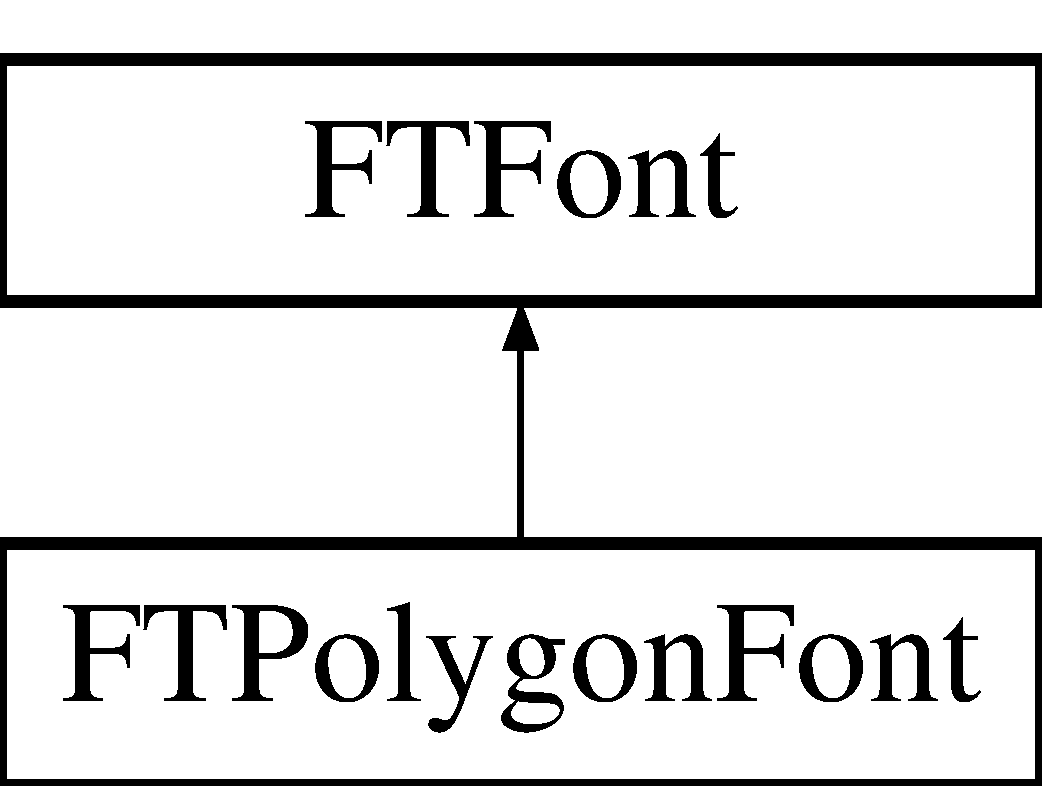
\includegraphics[height=2.000000cm]{classFTPolygonFont}
\end{center}
\end{figure}
\subsection*{Public Member Functions}
\begin{DoxyCompactItemize}
\item 
{\bf FTPolygonFont} (const char $\ast$fontFilePath)
\begin{DoxyCompactList}\small\item\em Open and read a font file. \item\end{DoxyCompactList}\item 
{\bf FTPolygonFont} (const unsigned char $\ast$pBufferBytes, size\_\-t bufferSizeInBytes)
\begin{DoxyCompactList}\small\item\em Open and read a font from a buffer in memory. \item\end{DoxyCompactList}\item 
{\bf $\sim$FTPolygonFont} ()
\begin{DoxyCompactList}\small\item\em Destructor. \item\end{DoxyCompactList}\end{DoxyCompactItemize}
\subsection*{Protected Member Functions}
\begin{DoxyCompactItemize}
\item 
virtual {\bf FTGlyph} $\ast$ {\bf MakeGlyph} (FT\_\-GlyphSlot slot)
\begin{DoxyCompactList}\small\item\em Construct a glyph of the correct type. \item\end{DoxyCompactList}\end{DoxyCompactItemize}


\subsection{Detailed Description}
\doxyref{FTPolygonFont}{p.}{classFTPolygonFont} is a specialisation of the \doxyref{FTFont}{p.}{classFTFont} class for handling tesselated Polygon Mesh fonts. \begin{DoxySeeAlso}{See also}
\doxyref{FTFont}{p.}{classFTFont} 
\end{DoxySeeAlso}


Definition at line 45 of file FTGLPolygonFont.h.



\subsection{Constructor \& Destructor Documentation}
\index{FTPolygonFont@{FTPolygonFont}!FTPolygonFont@{FTPolygonFont}}
\index{FTPolygonFont@{FTPolygonFont}!FTPolygonFont@{FTPolygonFont}}
\subsubsection[{FTPolygonFont}]{\setlength{\rightskip}{0pt plus 5cm}FTPolygonFont::FTPolygonFont (
\begin{DoxyParamCaption}
\item[{const char $\ast$}]{ fontFilePath}
\end{DoxyParamCaption}
)}\label{classFTPolygonFont_a69d65f22dcbe492b44cc0c7340d94d53}


Open and read a font file. 

Sets Error flag.


\begin{DoxyParams}{Parameters}
{\em fontFilePath} & font file path. \\
\hline
\end{DoxyParams}
\index{FTPolygonFont@{FTPolygonFont}!FTPolygonFont@{FTPolygonFont}}
\index{FTPolygonFont@{FTPolygonFont}!FTPolygonFont@{FTPolygonFont}}
\subsubsection[{FTPolygonFont}]{\setlength{\rightskip}{0pt plus 5cm}FTPolygonFont::FTPolygonFont (
\begin{DoxyParamCaption}
\item[{const unsigned char $\ast$}]{ pBufferBytes, }
\item[{size\_\-t}]{ bufferSizeInBytes}
\end{DoxyParamCaption}
)}\label{classFTPolygonFont_a462ed082228153dceec87ec1453e85b2}


Open and read a font from a buffer in memory. 

Sets Error flag. The buffer is owned by the client and is NOT copied by \doxyref{FTGL}{p.}{namespaceFTGL}. The pointer must be valid while using \doxyref{FTGL}{p.}{namespaceFTGL}.


\begin{DoxyParams}{Parameters}
{\em pBufferBytes} & the in-\/memory buffer \\
\hline
{\em bufferSizeInBytes} & the length of the buffer in bytes \\
\hline
\end{DoxyParams}
\index{FTPolygonFont@{FTPolygonFont}!$\sim$FTPolygonFont@{$\sim$FTPolygonFont}}
\index{$\sim$FTPolygonFont@{$\sim$FTPolygonFont}!FTPolygonFont@{FTPolygonFont}}
\subsubsection[{$\sim$FTPolygonFont}]{\setlength{\rightskip}{0pt plus 5cm}FTPolygonFont::$\sim$FTPolygonFont (
\begin{DoxyParamCaption}
{}
\end{DoxyParamCaption}
)}\label{classFTPolygonFont_ad71644a0d27c8f1791b9823cc7153cab}


Destructor. 



\subsection{Member Function Documentation}
\index{FTPolygonFont@{FTPolygonFont}!MakeGlyph@{MakeGlyph}}
\index{MakeGlyph@{MakeGlyph}!FTPolygonFont@{FTPolygonFont}}
\subsubsection[{MakeGlyph}]{\setlength{\rightskip}{0pt plus 5cm}virtual {\bf FTGlyph}$\ast$ FTPolygonFont::MakeGlyph (
\begin{DoxyParamCaption}
\item[{FT\_\-GlyphSlot}]{ slot}
\end{DoxyParamCaption}
)\hspace{0.3cm}{\ttfamily  [protected, virtual]}}\label{classFTPolygonFont_a3ce00692583b8cdddfffbe284c42ccf6}


Construct a glyph of the correct type. 

Clients must override the function and return their specialised \doxyref{FTGlyph}{p.}{classFTGlyph}.


\begin{DoxyParams}{Parameters}
{\em slot} & A FreeType glyph slot. \\
\hline
\end{DoxyParams}
\begin{DoxyReturn}{Returns}
An FT$\ast$$\ast$$\ast$$\ast$Glyph or {\ttfamily null} on failure. 
\end{DoxyReturn}


Implements {\bf FTFont} \doxyref{}{p.}{classFTFont_a07f8bef6c3bd52e7d905e6db17c9b8e6}.



The documentation for this class was generated from the following file:\begin{DoxyCompactItemize}
\item 
{\bf FTGLPolygonFont.h}\end{DoxyCompactItemize}

\section{FTPolygonGlyph Class Reference}
\label{classFTPolygonGlyph}\index{FTPolygonGlyph@{FTPolygonGlyph}}


\doxyref{FTPolygonGlyph}{p.}{classFTPolygonGlyph} is a specialisation of \doxyref{FTGlyph}{p.}{classFTGlyph} for creating tessellated polygon glyphs.  




{\ttfamily \#include $<$FTPolyGlyph.h$>$}

Inheritance diagram for FTPolygonGlyph:\begin{figure}[H]
\begin{center}
\leavevmode
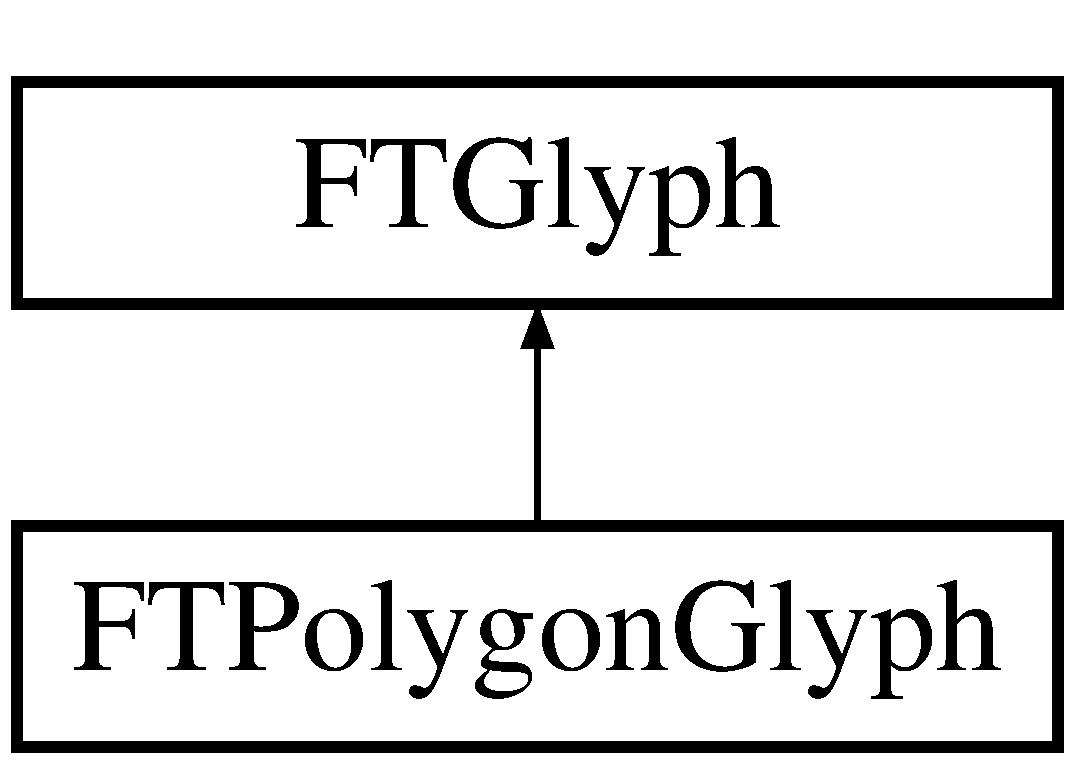
\includegraphics[height=2.000000cm]{classFTPolygonGlyph}
\end{center}
\end{figure}
\subsection*{Public Member Functions}
\begin{DoxyCompactItemize}
\item 
{\bf FTPolygonGlyph} (FT\_\-GlyphSlot glyph, float outset, bool useDisplayList)
\begin{DoxyCompactList}\small\item\em Constructor. \item\end{DoxyCompactList}\item 
virtual {\bf $\sim$FTPolygonGlyph} ()
\begin{DoxyCompactList}\small\item\em Destructor. \item\end{DoxyCompactList}\item 
virtual const {\bf FTPoint} \& {\bf Render} (const {\bf FTPoint} \&pen, int renderMode)
\begin{DoxyCompactList}\small\item\em Render this glyph at the current pen position. \item\end{DoxyCompactList}\end{DoxyCompactItemize}


\subsection{Detailed Description}
\doxyref{FTPolygonGlyph}{p.}{classFTPolygonGlyph} is a specialisation of \doxyref{FTGlyph}{p.}{classFTGlyph} for creating tessellated polygon glyphs. 

Definition at line 43 of file FTPolyGlyph.h.



\subsection{Constructor \& Destructor Documentation}
\index{FTPolygonGlyph@{FTPolygonGlyph}!FTPolygonGlyph@{FTPolygonGlyph}}
\index{FTPolygonGlyph@{FTPolygonGlyph}!FTPolygonGlyph@{FTPolygonGlyph}}
\subsubsection[{FTPolygonGlyph}]{\setlength{\rightskip}{0pt plus 5cm}FTPolygonGlyph::FTPolygonGlyph (
\begin{DoxyParamCaption}
\item[{FT\_\-GlyphSlot}]{ glyph, }
\item[{float}]{ outset, }
\item[{bool}]{ useDisplayList}
\end{DoxyParamCaption}
)}\label{classFTPolygonGlyph_ab3edfc4a5c2a03a714989324389b42ba}


Constructor. 

Sets the Error to Invalid\_\-Outline if the glyphs isn't an outline.


\begin{DoxyParams}{Parameters}
{\em glyph} & The Freetype glyph to be processed \\
\hline
{\em outset} & The outset distance \\
\hline
{\em useDisplayList} & Enable or disable the use of Display Lists for this glyph {\ttfamily true} turns ON display lists. {\ttfamily false} turns OFF display lists. \\
\hline
\end{DoxyParams}
\index{FTPolygonGlyph@{FTPolygonGlyph}!$\sim$FTPolygonGlyph@{$\sim$FTPolygonGlyph}}
\index{$\sim$FTPolygonGlyph@{$\sim$FTPolygonGlyph}!FTPolygonGlyph@{FTPolygonGlyph}}
\subsubsection[{$\sim$FTPolygonGlyph}]{\setlength{\rightskip}{0pt plus 5cm}virtual FTPolygonGlyph::$\sim$FTPolygonGlyph (
\begin{DoxyParamCaption}
{}
\end{DoxyParamCaption}
)\hspace{0.3cm}{\ttfamily  [virtual]}}\label{classFTPolygonGlyph_ab45178cf40ac634a73870d70cf09a80b}


Destructor. 



\subsection{Member Function Documentation}
\index{FTPolygonGlyph@{FTPolygonGlyph}!Render@{Render}}
\index{Render@{Render}!FTPolygonGlyph@{FTPolygonGlyph}}
\subsubsection[{Render}]{\setlength{\rightskip}{0pt plus 5cm}virtual const {\bf FTPoint}\& FTPolygonGlyph::Render (
\begin{DoxyParamCaption}
\item[{const {\bf FTPoint} \&}]{ pen, }
\item[{int}]{ renderMode}
\end{DoxyParamCaption}
)\hspace{0.3cm}{\ttfamily  [virtual]}}\label{classFTPolygonGlyph_ae790f0d5d4d85bafb7c63edf537255b7}


Render this glyph at the current pen position. 


\begin{DoxyParams}{Parameters}
{\em pen} & The current pen position. \\
\hline
{\em renderMode} & Render mode to display \\
\hline
\end{DoxyParams}
\begin{DoxyReturn}{Returns}
The advance distance for this glyph. 
\end{DoxyReturn}


Implements {\bf FTGlyph} \doxyref{}{p.}{classFTGlyph_abcf3aef56d4bf022f6d95d5e287800df}.



The documentation for this class was generated from the following file:\begin{DoxyCompactItemize}
\item 
{\bf FTPolyGlyph.h}\end{DoxyCompactItemize}

\section{FTSimpleLayout Class Reference}
\label{classFTSimpleLayout}\index{FTSimpleLayout@{FTSimpleLayout}}


\doxyref{FTSimpleLayout}{p.}{classFTSimpleLayout} is a specialisation of \doxyref{FTLayout}{p.}{classFTLayout} for simple text boxes.  




{\ttfamily \#include $<$FTSimpleLayout.h$>$}

Inheritance diagram for FTSimpleLayout:\begin{figure}[H]
\begin{center}
\leavevmode
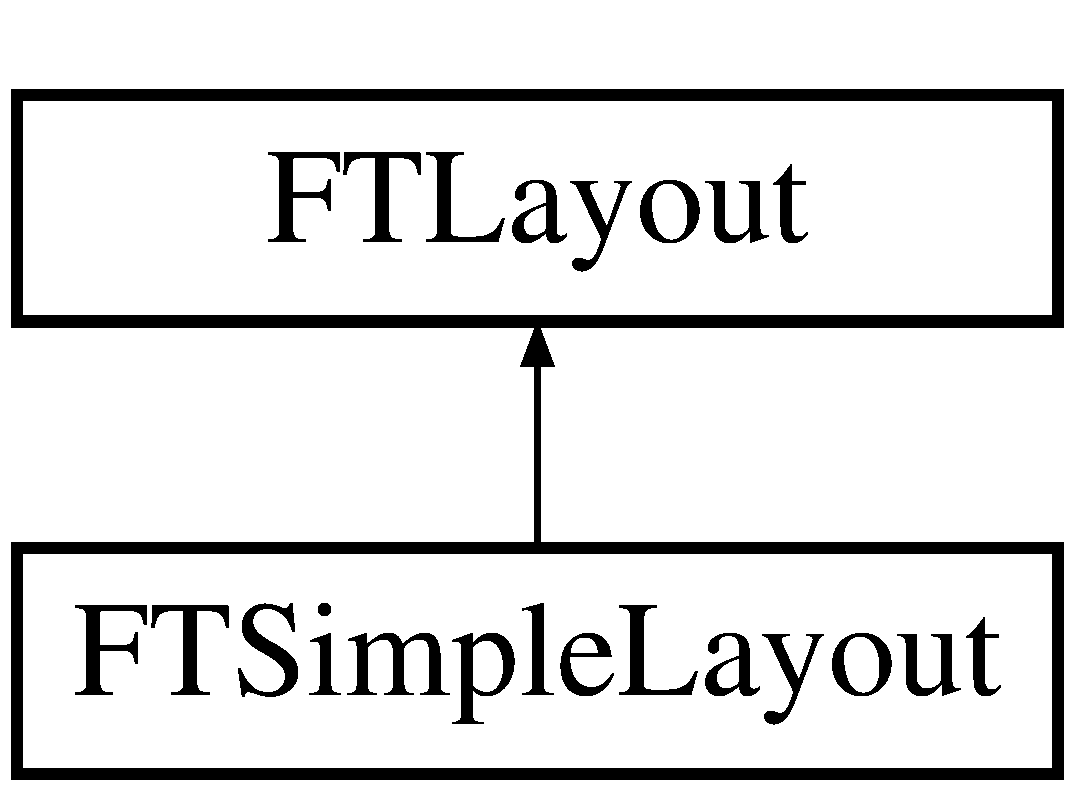
\includegraphics[height=2.000000cm]{classFTSimpleLayout}
\end{center}
\end{figure}
\subsection*{Public Member Functions}
\begin{DoxyCompactItemize}
\item 
{\bf FTSimpleLayout} ()
\begin{DoxyCompactList}\small\item\em Initializes line spacing to 1.0, alignment to ALIGN\_\-LEFT and wrap to 100.0. \item\end{DoxyCompactList}\item 
{\bf $\sim$FTSimpleLayout} ()
\begin{DoxyCompactList}\small\item\em Destructor. \item\end{DoxyCompactList}\item 
virtual {\bf FTBBox} {\bf BBox} (const char $\ast$string, const int len=-\/1, {\bf FTPoint} position={\bf FTPoint}())
\begin{DoxyCompactList}\small\item\em Get the bounding box for a formatted string. \item\end{DoxyCompactList}\item 
virtual {\bf FTBBox} {\bf BBox} (const wchar\_\-t $\ast$string, const int len=-\/1, {\bf FTPoint} position={\bf FTPoint}())
\begin{DoxyCompactList}\small\item\em Get the bounding box for a formatted string. \item\end{DoxyCompactList}\item 
virtual void {\bf Render} (const char $\ast$string, const int len=-\/1, {\bf FTPoint} position={\bf FTPoint}(), int renderMode=FTGL::RENDER\_\-ALL)
\begin{DoxyCompactList}\small\item\em Render a string of characters. \item\end{DoxyCompactList}\item 
virtual void {\bf Render} (const wchar\_\-t $\ast$string, const int len=-\/1, {\bf FTPoint} position={\bf FTPoint}(), int renderMode=FTGL::RENDER\_\-ALL)
\begin{DoxyCompactList}\small\item\em Render a string of characters. \item\end{DoxyCompactList}\item 
void {\bf SetFont} ({\bf FTFont} $\ast$fontInit)
\begin{DoxyCompactList}\small\item\em Set the font to use for rendering the text. \item\end{DoxyCompactList}\item 
{\bf FTFont} $\ast$ {\bf GetFont} ()
\item 
void {\bf SetLineLength} (const float LineLength)
\begin{DoxyCompactList}\small\item\em The maximum line length for formatting text. \item\end{DoxyCompactList}\item 
float {\bf GetLineLength} () const 
\item 
void {\bf SetAlignment} (const {\bf FTGL::TextAlignment} Alignment)
\begin{DoxyCompactList}\small\item\em The text alignment mode used to distribute space within a line or rendered text. \item\end{DoxyCompactList}\item 
{\bf FTGL::TextAlignment} {\bf GetAlignment} () const 
\item 
void {\bf SetLineSpacing} (const float LineSpacing)
\begin{DoxyCompactList}\small\item\em Sets the line height. \item\end{DoxyCompactList}\item 
float {\bf GetLineSpacing} () const 
\end{DoxyCompactItemize}


\subsection{Detailed Description}
\doxyref{FTSimpleLayout}{p.}{classFTSimpleLayout} is a specialisation of \doxyref{FTLayout}{p.}{classFTLayout} for simple text boxes. This class has basic support for text wrapping, left, right and centered alignment, and text justification.

\begin{DoxySeeAlso}{See also}
\doxyref{FTLayout}{p.}{classFTLayout} 
\end{DoxySeeAlso}


Definition at line 49 of file FTSimpleLayout.h.



\subsection{Constructor \& Destructor Documentation}
\index{FTSimpleLayout@{FTSimpleLayout}!FTSimpleLayout@{FTSimpleLayout}}
\index{FTSimpleLayout@{FTSimpleLayout}!FTSimpleLayout@{FTSimpleLayout}}
\subsubsection[{FTSimpleLayout}]{\setlength{\rightskip}{0pt plus 5cm}FTSimpleLayout::FTSimpleLayout (
\begin{DoxyParamCaption}
{}
\end{DoxyParamCaption}
)}\label{classFTSimpleLayout_a5627935363d9b0b3b7e02d1a237a3084}


Initializes line spacing to 1.0, alignment to ALIGN\_\-LEFT and wrap to 100.0. 

\index{FTSimpleLayout@{FTSimpleLayout}!$\sim$FTSimpleLayout@{$\sim$FTSimpleLayout}}
\index{$\sim$FTSimpleLayout@{$\sim$FTSimpleLayout}!FTSimpleLayout@{FTSimpleLayout}}
\subsubsection[{$\sim$FTSimpleLayout}]{\setlength{\rightskip}{0pt plus 5cm}FTSimpleLayout::$\sim$FTSimpleLayout (
\begin{DoxyParamCaption}
{}
\end{DoxyParamCaption}
)}\label{classFTSimpleLayout_af924484b92ee910a8261ed4d27ad94a8}


Destructor. 



\subsection{Member Function Documentation}
\index{FTSimpleLayout@{FTSimpleLayout}!BBox@{BBox}}
\index{BBox@{BBox}!FTSimpleLayout@{FTSimpleLayout}}
\subsubsection[{BBox}]{\setlength{\rightskip}{0pt plus 5cm}virtual {\bf FTBBox} FTSimpleLayout::BBox (
\begin{DoxyParamCaption}
\item[{const char $\ast$}]{ string, }
\item[{const int}]{ len = {\ttfamily -\/1}, }
\item[{{\bf FTPoint}}]{ position = {\ttfamily {\bf FTPoint}()}}
\end{DoxyParamCaption}
)\hspace{0.3cm}{\ttfamily  [virtual]}}\label{classFTSimpleLayout_a132c938c66912fe0b2360152349f887c}


Get the bounding box for a formatted string. 


\begin{DoxyParams}{Parameters}
{\em string} & A char string. \\
\hline
{\em len} & The length of the string. If $<$ 0 then all characters will be checked until a null character is encountered (optional). \\
\hline
{\em position} & The pen position of the first character (optional). \\
\hline
\end{DoxyParams}
\begin{DoxyReturn}{Returns}
The corresponding bounding box. 
\end{DoxyReturn}


Implements {\bf FTLayout} \doxyref{}{p.}{classFTLayout_ae79561f22ee39e69ce27d84b1d47fe2e}.

\index{FTSimpleLayout@{FTSimpleLayout}!BBox@{BBox}}
\index{BBox@{BBox}!FTSimpleLayout@{FTSimpleLayout}}
\subsubsection[{BBox}]{\setlength{\rightskip}{0pt plus 5cm}virtual {\bf FTBBox} FTSimpleLayout::BBox (
\begin{DoxyParamCaption}
\item[{const wchar\_\-t $\ast$}]{ string, }
\item[{const int}]{ len = {\ttfamily -\/1}, }
\item[{{\bf FTPoint}}]{ position = {\ttfamily {\bf FTPoint}()}}
\end{DoxyParamCaption}
)\hspace{0.3cm}{\ttfamily  [virtual]}}\label{classFTSimpleLayout_afdec41319af9fbeec0316e38d0661107}


Get the bounding box for a formatted string. 


\begin{DoxyParams}{Parameters}
{\em string} & A wchar\_\-t string. \\
\hline
{\em len} & The length of the string. If $<$ 0 then all characters will be checked until a null character is encountered (optional). \\
\hline
{\em position} & The pen position of the first character (optional). \\
\hline
\end{DoxyParams}
\begin{DoxyReturn}{Returns}
The corresponding bounding box. 
\end{DoxyReturn}


Implements {\bf FTLayout} \doxyref{}{p.}{classFTLayout_abf64582771a2281d901af1e074535c2a}.

\index{FTSimpleLayout@{FTSimpleLayout}!GetAlignment@{GetAlignment}}
\index{GetAlignment@{GetAlignment}!FTSimpleLayout@{FTSimpleLayout}}
\subsubsection[{GetAlignment}]{\setlength{\rightskip}{0pt plus 5cm}{\bf FTGL::TextAlignment} FTSimpleLayout::GetAlignment (
\begin{DoxyParamCaption}
{}
\end{DoxyParamCaption}
) const}\label{classFTSimpleLayout_a98afc657f353d719a84cba5576717a5b}
\begin{DoxyReturn}{Returns}
The text alignment mode. 
\end{DoxyReturn}
\index{FTSimpleLayout@{FTSimpleLayout}!GetFont@{GetFont}}
\index{GetFont@{GetFont}!FTSimpleLayout@{FTSimpleLayout}}
\subsubsection[{GetFont}]{\setlength{\rightskip}{0pt plus 5cm}{\bf FTFont}$\ast$ FTSimpleLayout::GetFont (
\begin{DoxyParamCaption}
{}
\end{DoxyParamCaption}
)}\label{classFTSimpleLayout_a0c14d2816d57c13ca71bef1e106d6ab3}
\begin{DoxyReturn}{Returns}
The current font. 
\end{DoxyReturn}
\index{FTSimpleLayout@{FTSimpleLayout}!GetLineLength@{GetLineLength}}
\index{GetLineLength@{GetLineLength}!FTSimpleLayout@{FTSimpleLayout}}
\subsubsection[{GetLineLength}]{\setlength{\rightskip}{0pt plus 5cm}float FTSimpleLayout::GetLineLength (
\begin{DoxyParamCaption}
{}
\end{DoxyParamCaption}
) const}\label{classFTSimpleLayout_acc1572a775a397847bfab19524f2fa62}
\begin{DoxyReturn}{Returns}
The current line length. 
\end{DoxyReturn}
\index{FTSimpleLayout@{FTSimpleLayout}!GetLineSpacing@{GetLineSpacing}}
\index{GetLineSpacing@{GetLineSpacing}!FTSimpleLayout@{FTSimpleLayout}}
\subsubsection[{GetLineSpacing}]{\setlength{\rightskip}{0pt plus 5cm}float FTSimpleLayout::GetLineSpacing (
\begin{DoxyParamCaption}
{}
\end{DoxyParamCaption}
) const}\label{classFTSimpleLayout_acb297d1855834539378de845182005c3}
\begin{DoxyReturn}{Returns}
The line spacing. 
\end{DoxyReturn}
\index{FTSimpleLayout@{FTSimpleLayout}!Render@{Render}}
\index{Render@{Render}!FTSimpleLayout@{FTSimpleLayout}}
\subsubsection[{Render}]{\setlength{\rightskip}{0pt plus 5cm}virtual void FTSimpleLayout::Render (
\begin{DoxyParamCaption}
\item[{const wchar\_\-t $\ast$}]{ string, }
\item[{const int}]{ len = {\ttfamily -\/1}, }
\item[{{\bf FTPoint}}]{ position = {\ttfamily {\bf FTPoint}()}, }
\item[{int}]{ renderMode = {\ttfamily FTGL::RENDER\_\-ALL}}
\end{DoxyParamCaption}
)\hspace{0.3cm}{\ttfamily  [virtual]}}\label{classFTSimpleLayout_aeea681385258bf9cd20c355555c9dbaf}


Render a string of characters. 


\begin{DoxyParams}{Parameters}
{\em string} & wchar\_\-t string to be output. \\
\hline
{\em len} & The length of the string. If $<$ 0 then all characters will be displayed until a null character is encountered (optional). \\
\hline
{\em position} & The pen position of the first character (optional). \\
\hline
{\em renderMode} & Render mode to display (optional) \\
\hline
\end{DoxyParams}


Implements {\bf FTLayout} \doxyref{}{p.}{classFTLayout_a793a7b371c885420d73acc56a667d53a}.

\index{FTSimpleLayout@{FTSimpleLayout}!Render@{Render}}
\index{Render@{Render}!FTSimpleLayout@{FTSimpleLayout}}
\subsubsection[{Render}]{\setlength{\rightskip}{0pt plus 5cm}virtual void FTSimpleLayout::Render (
\begin{DoxyParamCaption}
\item[{const char $\ast$}]{ string, }
\item[{const int}]{ len = {\ttfamily -\/1}, }
\item[{{\bf FTPoint}}]{ position = {\ttfamily {\bf FTPoint}()}, }
\item[{int}]{ renderMode = {\ttfamily FTGL::RENDER\_\-ALL}}
\end{DoxyParamCaption}
)\hspace{0.3cm}{\ttfamily  [virtual]}}\label{classFTSimpleLayout_afc122918b71e571155ca714eeb5c4888}


Render a string of characters. 


\begin{DoxyParams}{Parameters}
{\em string} & 'C' style string to be output. \\
\hline
{\em len} & The length of the string. If $<$ 0 then all characters will be displayed until a null character is encountered (optional). \\
\hline
{\em position} & The pen position of the first character (optional). \\
\hline
{\em renderMode} & Render mode to display (optional) \\
\hline
\end{DoxyParams}


Implements {\bf FTLayout} \doxyref{}{p.}{classFTLayout_a0e18bf877bbfe871e93ec0ebf1437a0f}.

\index{FTSimpleLayout@{FTSimpleLayout}!SetAlignment@{SetAlignment}}
\index{SetAlignment@{SetAlignment}!FTSimpleLayout@{FTSimpleLayout}}
\subsubsection[{SetAlignment}]{\setlength{\rightskip}{0pt plus 5cm}void FTSimpleLayout::SetAlignment (
\begin{DoxyParamCaption}
\item[{const {\bf FTGL::TextAlignment}}]{ Alignment}
\end{DoxyParamCaption}
)}\label{classFTSimpleLayout_a1aa39810095a4149d6795d159f3a8989}


The text alignment mode used to distribute space within a line or rendered text. 


\begin{DoxyParams}{Parameters}
{\em Alignment} & The new alignment mode. \\
\hline
\end{DoxyParams}
\index{FTSimpleLayout@{FTSimpleLayout}!SetFont@{SetFont}}
\index{SetFont@{SetFont}!FTSimpleLayout@{FTSimpleLayout}}
\subsubsection[{SetFont}]{\setlength{\rightskip}{0pt plus 5cm}void FTSimpleLayout::SetFont (
\begin{DoxyParamCaption}
\item[{{\bf FTFont} $\ast$}]{ fontInit}
\end{DoxyParamCaption}
)}\label{classFTSimpleLayout_a75492e803d5bc6dee379f2af1656c63d}


Set the font to use for rendering the text. 


\begin{DoxyParams}{Parameters}
{\em fontInit} & A pointer to the new font. The font is referenced by this but will not be disposed of when this is deleted. \\
\hline
\end{DoxyParams}
\index{FTSimpleLayout@{FTSimpleLayout}!SetLineLength@{SetLineLength}}
\index{SetLineLength@{SetLineLength}!FTSimpleLayout@{FTSimpleLayout}}
\subsubsection[{SetLineLength}]{\setlength{\rightskip}{0pt plus 5cm}void FTSimpleLayout::SetLineLength (
\begin{DoxyParamCaption}
\item[{const float}]{ LineLength}
\end{DoxyParamCaption}
)}\label{classFTSimpleLayout_afbe232e3486ce1afce63dae3a11cb0c0}


The maximum line length for formatting text. 


\begin{DoxyParams}{Parameters}
{\em LineLength} & The new line length. \\
\hline
\end{DoxyParams}
\index{FTSimpleLayout@{FTSimpleLayout}!SetLineSpacing@{SetLineSpacing}}
\index{SetLineSpacing@{SetLineSpacing}!FTSimpleLayout@{FTSimpleLayout}}
\subsubsection[{SetLineSpacing}]{\setlength{\rightskip}{0pt plus 5cm}void FTSimpleLayout::SetLineSpacing (
\begin{DoxyParamCaption}
\item[{const float}]{ LineSpacing}
\end{DoxyParamCaption}
)}\label{classFTSimpleLayout_a683607be7b7ee5c2272b63b3461ce749}


Sets the line height. 


\begin{DoxyParams}{Parameters}
{\em LineSpacing} & The height of each line of text expressed as a percentage of the current fonts line height. \\
\hline
\end{DoxyParams}


The documentation for this class was generated from the following file:\begin{DoxyCompactItemize}
\item 
{\bf FTSimpleLayout.h}\end{DoxyCompactItemize}

\section{FTTextureFont Class Reference}
\label{classFTTextureFont}\index{FTTextureFont@{FTTextureFont}}


\doxyref{FTTextureFont}{p.}{classFTTextureFont} is a specialisation of the \doxyref{FTFont}{p.}{classFTFont} class for handling Texture mapped fonts.  




{\ttfamily \#include $<$FTGLTextureFont.h$>$}

Inheritance diagram for FTTextureFont:\begin{figure}[H]
\begin{center}
\leavevmode
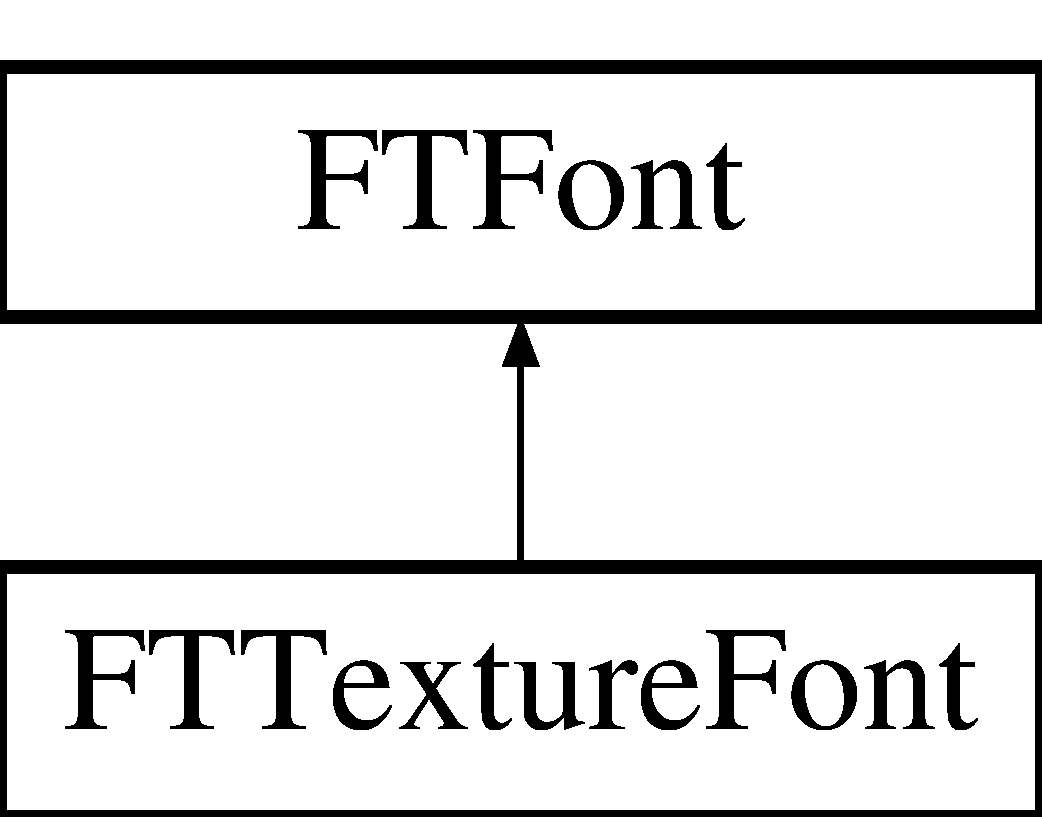
\includegraphics[height=2.000000cm]{classFTTextureFont}
\end{center}
\end{figure}
\subsection*{Public Member Functions}
\begin{DoxyCompactItemize}
\item 
{\bf FTTextureFont} (const char $\ast$fontFilePath)
\begin{DoxyCompactList}\small\item\em Open and read a font file. \item\end{DoxyCompactList}\item 
{\bf FTTextureFont} (const unsigned char $\ast$pBufferBytes, size\_\-t bufferSizeInBytes)
\begin{DoxyCompactList}\small\item\em Open and read a font from a buffer in memory. \item\end{DoxyCompactList}\item 
virtual {\bf $\sim$FTTextureFont} ()
\begin{DoxyCompactList}\small\item\em Destructor. \item\end{DoxyCompactList}\end{DoxyCompactItemize}
\subsection*{Protected Member Functions}
\begin{DoxyCompactItemize}
\item 
virtual {\bf FTGlyph} $\ast$ {\bf MakeGlyph} (FT\_\-GlyphSlot slot)
\begin{DoxyCompactList}\small\item\em Construct a glyph of the correct type. \item\end{DoxyCompactList}\end{DoxyCompactItemize}


\subsection{Detailed Description}
\doxyref{FTTextureFont}{p.}{classFTTextureFont} is a specialisation of the \doxyref{FTFont}{p.}{classFTFont} class for handling Texture mapped fonts. \begin{DoxySeeAlso}{See also}
\doxyref{FTFont}{p.}{classFTFont} 
\end{DoxySeeAlso}


Definition at line 45 of file FTGLTextureFont.h.



\subsection{Constructor \& Destructor Documentation}
\index{FTTextureFont@{FTTextureFont}!FTTextureFont@{FTTextureFont}}
\index{FTTextureFont@{FTTextureFont}!FTTextureFont@{FTTextureFont}}
\subsubsection[{FTTextureFont}]{\setlength{\rightskip}{0pt plus 5cm}FTTextureFont::FTTextureFont (
\begin{DoxyParamCaption}
\item[{const char $\ast$}]{ fontFilePath}
\end{DoxyParamCaption}
)}\label{classFTTextureFont_aa11644acda0fd096cc65af6e135346bf}


Open and read a font file. 

Sets Error flag.


\begin{DoxyParams}{Parameters}
{\em fontFilePath} & font file path. \\
\hline
\end{DoxyParams}
\index{FTTextureFont@{FTTextureFont}!FTTextureFont@{FTTextureFont}}
\index{FTTextureFont@{FTTextureFont}!FTTextureFont@{FTTextureFont}}
\subsubsection[{FTTextureFont}]{\setlength{\rightskip}{0pt plus 5cm}FTTextureFont::FTTextureFont (
\begin{DoxyParamCaption}
\item[{const unsigned char $\ast$}]{ pBufferBytes, }
\item[{size\_\-t}]{ bufferSizeInBytes}
\end{DoxyParamCaption}
)}\label{classFTTextureFont_a435d40b8d0b4fb0932ac54e5399afaae}


Open and read a font from a buffer in memory. 

Sets Error flag. The buffer is owned by the client and is NOT copied by \doxyref{FTGL}{p.}{namespaceFTGL}. The pointer must be valid while using \doxyref{FTGL}{p.}{namespaceFTGL}.


\begin{DoxyParams}{Parameters}
{\em pBufferBytes} & the in-\/memory buffer \\
\hline
{\em bufferSizeInBytes} & the length of the buffer in bytes \\
\hline
\end{DoxyParams}
\index{FTTextureFont@{FTTextureFont}!$\sim$FTTextureFont@{$\sim$FTTextureFont}}
\index{$\sim$FTTextureFont@{$\sim$FTTextureFont}!FTTextureFont@{FTTextureFont}}
\subsubsection[{$\sim$FTTextureFont}]{\setlength{\rightskip}{0pt plus 5cm}virtual FTTextureFont::$\sim$FTTextureFont (
\begin{DoxyParamCaption}
{}
\end{DoxyParamCaption}
)\hspace{0.3cm}{\ttfamily  [virtual]}}\label{classFTTextureFont_acfdd9bb8234363690f82853c9e9fa60f}


Destructor. 



\subsection{Member Function Documentation}
\index{FTTextureFont@{FTTextureFont}!MakeGlyph@{MakeGlyph}}
\index{MakeGlyph@{MakeGlyph}!FTTextureFont@{FTTextureFont}}
\subsubsection[{MakeGlyph}]{\setlength{\rightskip}{0pt plus 5cm}virtual {\bf FTGlyph}$\ast$ FTTextureFont::MakeGlyph (
\begin{DoxyParamCaption}
\item[{FT\_\-GlyphSlot}]{ slot}
\end{DoxyParamCaption}
)\hspace{0.3cm}{\ttfamily  [protected, virtual]}}\label{classFTTextureFont_a3873876ac71776fcb9a3afe6e6e726e6}


Construct a glyph of the correct type. 

Clients must override the function and return their specialised \doxyref{FTGlyph}{p.}{classFTGlyph}.


\begin{DoxyParams}{Parameters}
{\em slot} & A FreeType glyph slot. \\
\hline
\end{DoxyParams}
\begin{DoxyReturn}{Returns}
An FT$\ast$$\ast$$\ast$$\ast$Glyph or {\ttfamily null} on failure. 
\end{DoxyReturn}


Implements {\bf FTFont} \doxyref{}{p.}{classFTFont_a07f8bef6c3bd52e7d905e6db17c9b8e6}.



The documentation for this class was generated from the following file:\begin{DoxyCompactItemize}
\item 
{\bf FTGLTextureFont.h}\end{DoxyCompactItemize}

\section{FTTextureGlyph Class Reference}
\label{classFTTextureGlyph}\index{FTTextureGlyph@{FTTextureGlyph}}


\doxyref{FTTextureGlyph}{p.}{classFTTextureGlyph} is a specialisation of \doxyref{FTGlyph}{p.}{classFTGlyph} for creating texture glyphs.  




{\ttfamily \#include $<$FTTextureGlyph.h$>$}

Inheritance diagram for FTTextureGlyph:\begin{figure}[H]
\begin{center}
\leavevmode
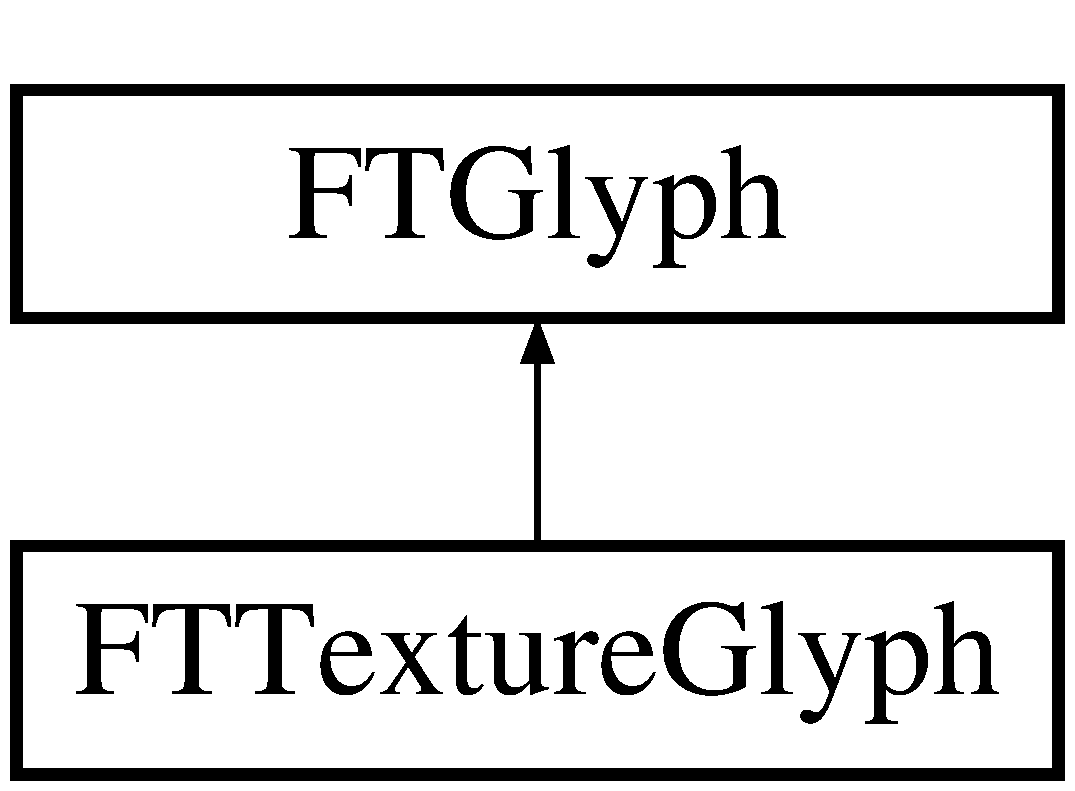
\includegraphics[height=2.000000cm]{classFTTextureGlyph}
\end{center}
\end{figure}
\subsection*{Public Member Functions}
\begin{DoxyCompactItemize}
\item 
{\bf FTTextureGlyph} (FT\_\-GlyphSlot glyph, int id, int xOffset, int yOffset, int width, int height)
\begin{DoxyCompactList}\small\item\em Constructor. \item\end{DoxyCompactList}\item 
virtual {\bf $\sim$FTTextureGlyph} ()
\begin{DoxyCompactList}\small\item\em Destructor. \item\end{DoxyCompactList}\item 
virtual const {\bf FTPoint} \& {\bf Render} (const {\bf FTPoint} \&pen, int renderMode)
\begin{DoxyCompactList}\small\item\em Render this glyph at the current pen position. \item\end{DoxyCompactList}\end{DoxyCompactItemize}


\subsection{Detailed Description}
\doxyref{FTTextureGlyph}{p.}{classFTTextureGlyph} is a specialisation of \doxyref{FTGlyph}{p.}{classFTGlyph} for creating texture glyphs. 

Definition at line 43 of file FTTextureGlyph.h.



\subsection{Constructor \& Destructor Documentation}
\index{FTTextureGlyph@{FTTextureGlyph}!FTTextureGlyph@{FTTextureGlyph}}
\index{FTTextureGlyph@{FTTextureGlyph}!FTTextureGlyph@{FTTextureGlyph}}
\subsubsection[{FTTextureGlyph}]{\setlength{\rightskip}{0pt plus 5cm}FTTextureGlyph::FTTextureGlyph (
\begin{DoxyParamCaption}
\item[{FT\_\-GlyphSlot}]{ glyph, }
\item[{int}]{ id, }
\item[{int}]{ xOffset, }
\item[{int}]{ yOffset, }
\item[{int}]{ width, }
\item[{int}]{ height}
\end{DoxyParamCaption}
)}\label{classFTTextureGlyph_a4e09ffe9a4cca361ea8052411c114b69}


Constructor. 


\begin{DoxyParams}{Parameters}
{\em glyph} & The Freetype glyph to be processed \\
\hline
{\em id} & The id of the texture that this glyph will be drawn in \\
\hline
{\em xOffset} & The x offset into the parent texture to draw this glyph \\
\hline
{\em yOffset} & The y offset into the parent texture to draw this glyph \\
\hline
{\em width} & The width of the parent texture \\
\hline
{\em height} & The height (number of rows) of the parent texture \\
\hline
\end{DoxyParams}
\index{FTTextureGlyph@{FTTextureGlyph}!$\sim$FTTextureGlyph@{$\sim$FTTextureGlyph}}
\index{$\sim$FTTextureGlyph@{$\sim$FTTextureGlyph}!FTTextureGlyph@{FTTextureGlyph}}
\subsubsection[{$\sim$FTTextureGlyph}]{\setlength{\rightskip}{0pt plus 5cm}virtual FTTextureGlyph::$\sim$FTTextureGlyph (
\begin{DoxyParamCaption}
{}
\end{DoxyParamCaption}
)\hspace{0.3cm}{\ttfamily  [virtual]}}\label{classFTTextureGlyph_ab0467ed99fc200ba43f2b0fb30f99eb9}


Destructor. 



\subsection{Member Function Documentation}
\index{FTTextureGlyph@{FTTextureGlyph}!Render@{Render}}
\index{Render@{Render}!FTTextureGlyph@{FTTextureGlyph}}
\subsubsection[{Render}]{\setlength{\rightskip}{0pt plus 5cm}virtual const {\bf FTPoint}\& FTTextureGlyph::Render (
\begin{DoxyParamCaption}
\item[{const {\bf FTPoint} \&}]{ pen, }
\item[{int}]{ renderMode}
\end{DoxyParamCaption}
)\hspace{0.3cm}{\ttfamily  [virtual]}}\label{classFTTextureGlyph_a23d91684651a5cc913e6232c60dc58f4}


Render this glyph at the current pen position. 


\begin{DoxyParams}{Parameters}
{\em pen} & The current pen position. \\
\hline
{\em renderMode} & Render mode to display \\
\hline
\end{DoxyParams}
\begin{DoxyReturn}{Returns}
The advance distance for this glyph. 
\end{DoxyReturn}


Implements {\bf FTGlyph} \doxyref{}{p.}{classFTGlyph_abcf3aef56d4bf022f6d95d5e287800df}.



The documentation for this class was generated from the following file:\begin{DoxyCompactItemize}
\item 
{\bf FTTextureGlyph.h}\end{DoxyCompactItemize}

\chapter{File Documentation}
\section{faq.dox File Reference}
\label{faq_8dox}\index{faq.dox@{faq.dox}}

\section{FTBBox.h File Reference}
\label{FTBBox_8h}\index{FTBBox.h@{FTBBox.h}}
{\ttfamily \#include $<$FTGL/ftgl.h$>$}\par
\subsection*{Data Structures}
\begin{DoxyCompactItemize}
\item 
class {\bf FTBBox}
\begin{DoxyCompactList}\small\item\em \doxyref{FTBBox}{p.}{classFTBBox} is a convenience class for handling bounding boxes. \item\end{DoxyCompactList}\end{DoxyCompactItemize}

\section{FTBitmapGlyph.h File Reference}
\label{FTBitmapGlyph_8h}\index{FTBitmapGlyph.h@{FTBitmapGlyph.h}}
{\ttfamily \#include $<$FTGL/ftgl.h$>$}\par
\subsection*{Data Structures}
\begin{DoxyCompactItemize}
\item 
class {\bf FTBitmapGlyph}
\begin{DoxyCompactList}\small\item\em \doxyref{FTBitmapGlyph}{p.}{classFTBitmapGlyph} is a specialisation of \doxyref{FTGlyph}{p.}{classFTGlyph} for creating bitmaps. \item\end{DoxyCompactList}\end{DoxyCompactItemize}
\subsection*{Functions}
\begin{DoxyCompactItemize}
\item 
{\bf FTGLglyph} $\ast$ {\bf ftglCreateBitmapGlyph} (FT\_\-GlyphSlot glyph)
\begin{DoxyCompactList}\small\item\em Create a specialisation of FTGLglyph for creating bitmaps. \item\end{DoxyCompactList}\end{DoxyCompactItemize}


\subsection{Function Documentation}
\index{FTBitmapGlyph.h@{FTBitmapGlyph.h}!ftglCreateBitmapGlyph@{ftglCreateBitmapGlyph}}
\index{ftglCreateBitmapGlyph@{ftglCreateBitmapGlyph}!FTBitmapGlyph.h@{FTBitmapGlyph.h}}
\subsubsection[{ftglCreateBitmapGlyph}]{\setlength{\rightskip}{0pt plus 5cm}{\bf FTGLglyph}$\ast$ ftglCreateBitmapGlyph (
\begin{DoxyParamCaption}
\item[{FT\_\-GlyphSlot}]{ glyph}
\end{DoxyParamCaption}
)}\label{FTBitmapGlyph_8h_afc2f914a981c1e942b5be71c02c5bda9}


Create a specialisation of FTGLglyph for creating bitmaps. 


\begin{DoxyParams}{Parameters}
{\em glyph} & The Freetype glyph to be processed \\
\hline
\end{DoxyParams}
\begin{DoxyReturn}{Returns}
An FTGLglyph$\ast$ object. 
\end{DoxyReturn}

\section{FTBuffer.h File Reference}
\label{FTBuffer_8h}\index{FTBuffer.h@{FTBuffer.h}}
{\ttfamily \#include $<$FTGL/ftgl.h$>$}\par
\subsection*{Data Structures}
\begin{DoxyCompactItemize}
\item 
class {\bf FTBuffer}
\begin{DoxyCompactList}\small\item\em \doxyref{FTBuffer}{p.}{classFTBuffer} is a helper class for pixel buffers. \item\end{DoxyCompactList}\end{DoxyCompactItemize}

\section{FTBufferFont.h File Reference}
\label{FTBufferFont_8h}\index{FTBufferFont.h@{FTBufferFont.h}}
{\ttfamily \#include $<$FTGL/ftgl.h$>$}\par
\subsection*{Data Structures}
\begin{DoxyCompactItemize}
\item 
class {\bf FTBufferFont}
\begin{DoxyCompactList}\small\item\em \doxyref{FTBufferFont}{p.}{classFTBufferFont} is a specialisation of the \doxyref{FTFont}{p.}{classFTFont} class for handling memory buffer fonts. \item\end{DoxyCompactList}\end{DoxyCompactItemize}
\subsection*{Functions}
\begin{DoxyCompactItemize}
\item 
{\bf FTGLfont} $\ast$ {\bf ftglCreateBufferFont} (const char $\ast$file)
\begin{DoxyCompactList}\small\item\em Create a specialised FTGLfont object for handling memory buffer fonts. \item\end{DoxyCompactList}\end{DoxyCompactItemize}


\subsection{Function Documentation}
\index{FTBufferFont.h@{FTBufferFont.h}!ftglCreateBufferFont@{ftglCreateBufferFont}}
\index{ftglCreateBufferFont@{ftglCreateBufferFont}!FTBufferFont.h@{FTBufferFont.h}}
\subsubsection[{ftglCreateBufferFont}]{\setlength{\rightskip}{0pt plus 5cm}{\bf FTGLfont}$\ast$ ftglCreateBufferFont (
\begin{DoxyParamCaption}
\item[{const char $\ast$}]{ file}
\end{DoxyParamCaption}
)}\label{FTBufferFont_8h_a163bd4dbfc2d258d71b265fcb9bbc5b7}


Create a specialised FTGLfont object for handling memory buffer fonts. 


\begin{DoxyParams}{Parameters}
{\em file} & The font file name. \\
\hline
\end{DoxyParams}
\begin{DoxyReturn}{Returns}
An FTGLfont$\ast$ object.
\end{DoxyReturn}
\begin{DoxySeeAlso}{See also}
\doxyref{FTGLfont}{p.}{FTFont_8h_af121f8e0374785b92e3155992d703b17} 
\end{DoxySeeAlso}

\section{FTBufferGlyph.h File Reference}
\label{FTBufferGlyph_8h}\index{FTBufferGlyph.h@{FTBufferGlyph.h}}
{\ttfamily \#include $<$FTGL/ftgl.h$>$}\par
\subsection*{Data Structures}
\begin{DoxyCompactItemize}
\item 
class {\bf FTBufferGlyph}
\begin{DoxyCompactList}\small\item\em \doxyref{FTBufferGlyph}{p.}{classFTBufferGlyph} is a specialisation of \doxyref{FTGlyph}{p.}{classFTGlyph} for memory buffer rendering. \item\end{DoxyCompactList}\end{DoxyCompactItemize}

\section{FTExtrdGlyph.h File Reference}
\label{FTExtrdGlyph_8h}\index{FTExtrdGlyph.h@{FTExtrdGlyph.h}}
{\ttfamily \#include $<$FTGL/ftgl.h$>$}\par
\subsection*{Data Structures}
\begin{DoxyCompactItemize}
\item 
class {\bf FTExtrudeGlyph}
\begin{DoxyCompactList}\small\item\em \doxyref{FTExtrudeGlyph}{p.}{classFTExtrudeGlyph} is a specialisation of \doxyref{FTGlyph}{p.}{classFTGlyph} for creating tessellated extruded polygon glyphs. \item\end{DoxyCompactList}\end{DoxyCompactItemize}
\subsection*{Defines}
\begin{DoxyCompactItemize}
\item 
\#define {\bf FTExtrdGlyph}~{\bf FTExtrudeGlyph}
\end{DoxyCompactItemize}
\subsection*{Functions}
\begin{DoxyCompactItemize}
\item 
{\bf FTGLglyph} $\ast$ {\bf ftglCreateExtrudeGlyph} (FT\_\-GlyphSlot glyph, float depth, float frontOutset, float backOutset, int useDisplayList)
\begin{DoxyCompactList}\small\item\em Create a specialisation of FTGLglyph for creating tessellated extruded polygon glyphs. \item\end{DoxyCompactList}\end{DoxyCompactItemize}


\subsection{Define Documentation}
\index{FTExtrdGlyph.h@{FTExtrdGlyph.h}!FTExtrdGlyph@{FTExtrdGlyph}}
\index{FTExtrdGlyph@{FTExtrdGlyph}!FTExtrdGlyph.h@{FTExtrdGlyph.h}}
\subsubsection[{FTExtrdGlyph}]{\setlength{\rightskip}{0pt plus 5cm}\#define FTExtrdGlyph~{\bf FTExtrudeGlyph}}\label{FTExtrdGlyph_8h_a8ef94254dc520e02f8013247b660081e}


Definition at line 77 of file FTExtrdGlyph.h.



\subsection{Function Documentation}
\index{FTExtrdGlyph.h@{FTExtrdGlyph.h}!ftglCreateExtrudeGlyph@{ftglCreateExtrudeGlyph}}
\index{ftglCreateExtrudeGlyph@{ftglCreateExtrudeGlyph}!FTExtrdGlyph.h@{FTExtrdGlyph.h}}
\subsubsection[{ftglCreateExtrudeGlyph}]{\setlength{\rightskip}{0pt plus 5cm}{\bf FTGLglyph}$\ast$ ftglCreateExtrudeGlyph (
\begin{DoxyParamCaption}
\item[{FT\_\-GlyphSlot}]{ glyph, }
\item[{float}]{ depth, }
\item[{float}]{ frontOutset, }
\item[{float}]{ backOutset, }
\item[{int}]{ useDisplayList}
\end{DoxyParamCaption}
)}\label{FTExtrdGlyph_8h_a325fc3b9c3a867c2d947e4c97caee92e}


Create a specialisation of FTGLglyph for creating tessellated extruded polygon glyphs. 


\begin{DoxyParams}{Parameters}
{\em glyph} & The Freetype glyph to be processed \\
\hline
{\em depth} & The distance along the z axis to extrude the glyph \\
\hline
{\em frontOutset} & outset contour size \\
\hline
{\em backOutset} & outset contour size \\
\hline
{\em useDisplayList} & Enable or disable the use of Display Lists for this glyph {\ttfamily true} turns ON display lists. {\ttfamily false} turns OFF display lists. \\
\hline
\end{DoxyParams}
\begin{DoxyReturn}{Returns}
An FTGLglyph$\ast$ object. 
\end{DoxyReturn}

\section{FTFont.h File Reference}
\label{FTFont_8h}\index{FTFont.h@{FTFont.h}}
{\ttfamily \#include $<$FTGL/ftgl.h$>$}\par
\subsection*{Data Structures}
\begin{DoxyCompactItemize}
\item 
class {\bf FTFont}
\begin{DoxyCompactList}\small\item\em \doxyref{FTFont}{p.}{classFTFont} is the public interface for the \doxyref{FTGL}{p.}{namespaceFTGL} library. \item\end{DoxyCompactList}\end{DoxyCompactItemize}
\subsection*{Typedefs}
\begin{DoxyCompactItemize}
\item 
typedef struct \_\-FTGLfont {\bf FTGLfont}
\end{DoxyCompactItemize}
\subsection*{Functions}
\begin{DoxyCompactItemize}
\item 
{\bf FTGLfont} $\ast$ {\bf ftglCreateCustomFont} (char const $\ast$fontFilePath, void $\ast$data, {\bf FTGLglyph} $\ast$($\ast$makeglyphCallback)(FT\_\-GlyphSlot, void $\ast$))
\begin{DoxyCompactList}\small\item\em Create a custom \doxyref{FTGL}{p.}{namespaceFTGL} font object. \item\end{DoxyCompactList}\item 
void {\bf ftglDestroyFont} ({\bf FTGLfont} $\ast$font)
\begin{DoxyCompactList}\small\item\em Destroy an \doxyref{FTGL}{p.}{namespaceFTGL} font object. \item\end{DoxyCompactList}\item 
int {\bf ftglAttachFile} ({\bf FTGLfont} $\ast$font, const char $\ast$path)
\begin{DoxyCompactList}\small\item\em Attach auxilliary file to font e.g. \item\end{DoxyCompactList}\item 
int {\bf ftglAttachData} ({\bf FTGLfont} $\ast$font, const unsigned char $\ast$data, size\_\-t size)
\begin{DoxyCompactList}\small\item\em Attach auxilliary data to font, e.g. \item\end{DoxyCompactList}\item 
int {\bf ftglSetFontCharMap} ({\bf FTGLfont} $\ast$font, FT\_\-Encoding encoding)
\begin{DoxyCompactList}\small\item\em Set the character map for the face. \item\end{DoxyCompactList}\item 
unsigned int {\bf ftglGetFontCharMapCount} ({\bf FTGLfont} $\ast$font)
\begin{DoxyCompactList}\small\item\em Get the number of character maps in this face. \item\end{DoxyCompactList}\item 
FT\_\-Encoding $\ast$ {\bf ftglGetFontCharMapList} ({\bf FTGLfont} $\ast$font)
\begin{DoxyCompactList}\small\item\em Get a list of character maps in this face. \item\end{DoxyCompactList}\item 
int {\bf ftglSetFontFaceSize} ({\bf FTGLfont} $\ast$font, unsigned int size, unsigned int res)
\begin{DoxyCompactList}\small\item\em Set the char size for the current face. \item\end{DoxyCompactList}\item 
unsigned int {\bf ftglGetFontFaceSize} ({\bf FTGLfont} $\ast$font)
\begin{DoxyCompactList}\small\item\em Get the current face size in points (1/72 inch). \item\end{DoxyCompactList}\item 
void {\bf ftglSetFontDepth} ({\bf FTGLfont} $\ast$font, float depth)
\begin{DoxyCompactList}\small\item\em Set the extrusion distance for the font. \item\end{DoxyCompactList}\item 
void {\bf ftglSetFontOutset} ({\bf FTGLfont} $\ast$font, float front, float back)
\begin{DoxyCompactList}\small\item\em Set the outset distance for the font. \item\end{DoxyCompactList}\item 
void {\bf ftglSetFontDisplayList} ({\bf FTGLfont} $\ast$font, int useList)
\begin{DoxyCompactList}\small\item\em Enable or disable the use of Display Lists inside \doxyref{FTGL}{p.}{namespaceFTGL}. \item\end{DoxyCompactList}\item 
float {\bf ftglGetFontAscender} ({\bf FTGLfont} $\ast$font)
\begin{DoxyCompactList}\small\item\em Get the global ascender height for the face. \item\end{DoxyCompactList}\item 
float {\bf ftglGetFontDescender} ({\bf FTGLfont} $\ast$font)
\begin{DoxyCompactList}\small\item\em Gets the global descender height for the face. \item\end{DoxyCompactList}\item 
float {\bf ftglGetFontLineHeight} ({\bf FTGLfont} $\ast$font)
\begin{DoxyCompactList}\small\item\em Gets the line spacing for the font. \item\end{DoxyCompactList}\item 
void {\bf ftglGetFontBBox} ({\bf FTGLfont} $\ast$font, const char $\ast$string, int len, float bounds[6])
\begin{DoxyCompactList}\small\item\em Get the bounding box for a string. \item\end{DoxyCompactList}\item 
float {\bf ftglGetFontAdvance} ({\bf FTGLfont} $\ast$font, const char $\ast$string)
\begin{DoxyCompactList}\small\item\em Get the advance width for a string. \item\end{DoxyCompactList}\item 
void {\bf ftglRenderFont} ({\bf FTGLfont} $\ast$font, const char $\ast$string, int mode)
\begin{DoxyCompactList}\small\item\em Render a string of characters. \item\end{DoxyCompactList}\item 
FT\_\-Error {\bf ftglGetFontError} ({\bf FTGLfont} $\ast$font)
\begin{DoxyCompactList}\small\item\em Query a font for errors. \item\end{DoxyCompactList}\end{DoxyCompactItemize}


\subsection{Typedef Documentation}
\index{FTFont.h@{FTFont.h}!FTGLfont@{FTGLfont}}
\index{FTGLfont@{FTGLfont}!FTFont.h@{FTFont.h}}
\subsubsection[{FTGLfont}]{\setlength{\rightskip}{0pt plus 5cm}typedef struct \_\-FTGLfont {\bf FTGLfont}}\label{FTFont_8h_af121f8e0374785b92e3155992d703b17}


Definition at line 399 of file FTFont.h.



\subsection{Function Documentation}
\index{FTFont.h@{FTFont.h}!ftglAttachData@{ftglAttachData}}
\index{ftglAttachData@{ftglAttachData}!FTFont.h@{FTFont.h}}
\subsubsection[{ftglAttachData}]{\setlength{\rightskip}{0pt plus 5cm}int ftglAttachData (
\begin{DoxyParamCaption}
\item[{{\bf FTGLfont} $\ast$}]{ font, }
\item[{const unsigned char $\ast$}]{ data, }
\item[{size\_\-t}]{ size}
\end{DoxyParamCaption}
)}\label{FTFont_8h_ad9fba15428fb163a34f9ee824e748162}


Attach auxilliary data to font, e.g. 

font metrics, from memory.

Note: not all font formats implement this function.


\begin{DoxyParams}{Parameters}
{\em font} & An FTGLfont$\ast$ object. \\
\hline
{\em data} & The in-\/memory buffer. \\
\hline
{\em size} & The length of the buffer in bytes. \\
\hline
\end{DoxyParams}
\begin{DoxyReturn}{Returns}
1 if file has been attached successfully. 
\end{DoxyReturn}
\index{FTFont.h@{FTFont.h}!ftglAttachFile@{ftglAttachFile}}
\index{ftglAttachFile@{ftglAttachFile}!FTFont.h@{FTFont.h}}
\subsubsection[{ftglAttachFile}]{\setlength{\rightskip}{0pt plus 5cm}int ftglAttachFile (
\begin{DoxyParamCaption}
\item[{{\bf FTGLfont} $\ast$}]{ font, }
\item[{const char $\ast$}]{ path}
\end{DoxyParamCaption}
)}\label{FTFont_8h_a4452c327ff636fc2f0ecb1859687bfe0}


Attach auxilliary file to font e.g. 

font metrics.

Note: not all font formats implement this function.


\begin{DoxyParams}{Parameters}
{\em font} & An FTGLfont$\ast$ object. \\
\hline
{\em path} & Auxilliary font file path. \\
\hline
\end{DoxyParams}
\begin{DoxyReturn}{Returns}
1 if file has been attached successfully. 
\end{DoxyReturn}
\index{FTFont.h@{FTFont.h}!ftglCreateCustomFont@{ftglCreateCustomFont}}
\index{ftglCreateCustomFont@{ftglCreateCustomFont}!FTFont.h@{FTFont.h}}
\subsubsection[{ftglCreateCustomFont}]{\setlength{\rightskip}{0pt plus 5cm}{\bf FTGLfont}$\ast$ ftglCreateCustomFont (
\begin{DoxyParamCaption}
\item[{char const $\ast$}]{ fontFilePath, }
\item[{void $\ast$}]{ data, }
\item[{{\bf FTGLglyph} $\ast$($\ast$)(FT\_\-GlyphSlot, void $\ast$)}]{ makeglyphCallback}
\end{DoxyParamCaption}
)}\label{FTFont_8h_a3f54c50d3bfa9b5c0b103b0f9a2debb2}


Create a custom \doxyref{FTGL}{p.}{namespaceFTGL} font object. 


\begin{DoxyParams}{Parameters}
{\em fontFilePath} & The font file name. \\
\hline
{\em data} & A pointer to private data that will be passed to callbacks. \\
\hline
{\em makeglyphCallback} & A glyph-\/making callback function. \\
\hline
\end{DoxyParams}
\begin{DoxyReturn}{Returns}
An FTGLfont$\ast$ object. 
\end{DoxyReturn}
\index{FTFont.h@{FTFont.h}!ftglDestroyFont@{ftglDestroyFont}}
\index{ftglDestroyFont@{ftglDestroyFont}!FTFont.h@{FTFont.h}}
\subsubsection[{ftglDestroyFont}]{\setlength{\rightskip}{0pt plus 5cm}void ftglDestroyFont (
\begin{DoxyParamCaption}
\item[{{\bf FTGLfont} $\ast$}]{ font}
\end{DoxyParamCaption}
)}\label{FTFont_8h_af0dc4b1c8987895d19e863416ae8d174}


Destroy an \doxyref{FTGL}{p.}{namespaceFTGL} font object. 


\begin{DoxyParams}{Parameters}
{\em font} & An FTGLfont$\ast$ object. \\
\hline
\end{DoxyParams}
\index{FTFont.h@{FTFont.h}!ftglGetFontAdvance@{ftglGetFontAdvance}}
\index{ftglGetFontAdvance@{ftglGetFontAdvance}!FTFont.h@{FTFont.h}}
\subsubsection[{ftglGetFontAdvance}]{\setlength{\rightskip}{0pt plus 5cm}float ftglGetFontAdvance (
\begin{DoxyParamCaption}
\item[{{\bf FTGLfont} $\ast$}]{ font, }
\item[{const char $\ast$}]{ string}
\end{DoxyParamCaption}
)}\label{FTFont_8h_a0886ea1dd82291182b2c9acd43f24571}


Get the advance width for a string. 


\begin{DoxyParams}{Parameters}
{\em font} & An FTGLfont$\ast$ object. \\
\hline
{\em string} & A char string. \\
\hline
\end{DoxyParams}
\begin{DoxyReturn}{Returns}
Advance width 
\end{DoxyReturn}
\index{FTFont.h@{FTFont.h}!ftglGetFontAscender@{ftglGetFontAscender}}
\index{ftglGetFontAscender@{ftglGetFontAscender}!FTFont.h@{FTFont.h}}
\subsubsection[{ftglGetFontAscender}]{\setlength{\rightskip}{0pt plus 5cm}float ftglGetFontAscender (
\begin{DoxyParamCaption}
\item[{{\bf FTGLfont} $\ast$}]{ font}
\end{DoxyParamCaption}
)}\label{FTFont_8h_a6f931a3b2bfad1511e80324717a7f00e}


Get the global ascender height for the face. 


\begin{DoxyParams}{Parameters}
{\em font} & An FTGLfont$\ast$ object. \\
\hline
\end{DoxyParams}
\begin{DoxyReturn}{Returns}
Ascender height 
\end{DoxyReturn}
\index{FTFont.h@{FTFont.h}!ftglGetFontBBox@{ftglGetFontBBox}}
\index{ftglGetFontBBox@{ftglGetFontBBox}!FTFont.h@{FTFont.h}}
\subsubsection[{ftglGetFontBBox}]{\setlength{\rightskip}{0pt plus 5cm}void ftglGetFontBBox (
\begin{DoxyParamCaption}
\item[{{\bf FTGLfont} $\ast$}]{ font, }
\item[{const char $\ast$}]{ string, }
\item[{int}]{ len, }
\item[{float}]{ bounds[6]}
\end{DoxyParamCaption}
)}\label{FTFont_8h_ae2f41b36c47bb3cbcb6f3e7f3d12ed74}


Get the bounding box for a string. 


\begin{DoxyParams}{Parameters}
{\em font} & An FTGLfont$\ast$ object. \\
\hline
{\em string} & A char buffer \\
\hline
{\em len} & The length of the string. If $<$ 0 then all characters will be checked until a null character is encountered (optional). \\
\hline
{\em bounds} & An array of 6 float values where the bounding box's lower left near and upper right far 3D coordinates will be stored. \\
\hline
\end{DoxyParams}
\index{FTFont.h@{FTFont.h}!ftglGetFontCharMapCount@{ftglGetFontCharMapCount}}
\index{ftglGetFontCharMapCount@{ftglGetFontCharMapCount}!FTFont.h@{FTFont.h}}
\subsubsection[{ftglGetFontCharMapCount}]{\setlength{\rightskip}{0pt plus 5cm}unsigned int ftglGetFontCharMapCount (
\begin{DoxyParamCaption}
\item[{{\bf FTGLfont} $\ast$}]{ font}
\end{DoxyParamCaption}
)}\label{FTFont_8h_a1ebde0e8531774259e234ccd9d067624}


Get the number of character maps in this face. 


\begin{DoxyParams}{Parameters}
{\em font} & An FTGLfont$\ast$ object. \\
\hline
\end{DoxyParams}
\begin{DoxyReturn}{Returns}
character map count. 
\end{DoxyReturn}
\index{FTFont.h@{FTFont.h}!ftglGetFontCharMapList@{ftglGetFontCharMapList}}
\index{ftglGetFontCharMapList@{ftglGetFontCharMapList}!FTFont.h@{FTFont.h}}
\subsubsection[{ftglGetFontCharMapList}]{\setlength{\rightskip}{0pt plus 5cm}FT\_\-Encoding$\ast$ ftglGetFontCharMapList (
\begin{DoxyParamCaption}
\item[{{\bf FTGLfont} $\ast$}]{ font}
\end{DoxyParamCaption}
)}\label{FTFont_8h_a7c7657c95cdbf9f4f84b4754cddc7aca}


Get a list of character maps in this face. 


\begin{DoxyParams}{Parameters}
{\em font} & An FTGLfont$\ast$ object. \\
\hline
\end{DoxyParams}
\begin{DoxyReturn}{Returns}
pointer to the first encoding. 
\end{DoxyReturn}
\index{FTFont.h@{FTFont.h}!ftglGetFontDescender@{ftglGetFontDescender}}
\index{ftglGetFontDescender@{ftglGetFontDescender}!FTFont.h@{FTFont.h}}
\subsubsection[{ftglGetFontDescender}]{\setlength{\rightskip}{0pt plus 5cm}float ftglGetFontDescender (
\begin{DoxyParamCaption}
\item[{{\bf FTGLfont} $\ast$}]{ font}
\end{DoxyParamCaption}
)}\label{FTFont_8h_a210968a0e92685b9b8522c869708425a}


Gets the global descender height for the face. 


\begin{DoxyParams}{Parameters}
{\em font} & An FTGLfont$\ast$ object. \\
\hline
\end{DoxyParams}
\begin{DoxyReturn}{Returns}
Descender height 
\end{DoxyReturn}
\index{FTFont.h@{FTFont.h}!ftglGetFontError@{ftglGetFontError}}
\index{ftglGetFontError@{ftglGetFontError}!FTFont.h@{FTFont.h}}
\subsubsection[{ftglGetFontError}]{\setlength{\rightskip}{0pt plus 5cm}FT\_\-Error ftglGetFontError (
\begin{DoxyParamCaption}
\item[{{\bf FTGLfont} $\ast$}]{ font}
\end{DoxyParamCaption}
)}\label{FTFont_8h_a7c334b38242e448749165dfdac5054fc}


Query a font for errors. 


\begin{DoxyParams}{Parameters}
{\em font} & An FTGLfont$\ast$ object. \\
\hline
\end{DoxyParams}
\begin{DoxyReturn}{Returns}
The current error code. 
\end{DoxyReturn}
\index{FTFont.h@{FTFont.h}!ftglGetFontFaceSize@{ftglGetFontFaceSize}}
\index{ftglGetFontFaceSize@{ftglGetFontFaceSize}!FTFont.h@{FTFont.h}}
\subsubsection[{ftglGetFontFaceSize}]{\setlength{\rightskip}{0pt plus 5cm}unsigned int ftglGetFontFaceSize (
\begin{DoxyParamCaption}
\item[{{\bf FTGLfont} $\ast$}]{ font}
\end{DoxyParamCaption}
)}\label{FTFont_8h_a8440b2e4f21d60eb9e3efc6ca9666bee}


Get the current face size in points (1/72 inch). 


\begin{DoxyParams}{Parameters}
{\em font} & An FTGLfont$\ast$ object. \\
\hline
\end{DoxyParams}
\begin{DoxyReturn}{Returns}
face size 
\end{DoxyReturn}
\index{FTFont.h@{FTFont.h}!ftglGetFontLineHeight@{ftglGetFontLineHeight}}
\index{ftglGetFontLineHeight@{ftglGetFontLineHeight}!FTFont.h@{FTFont.h}}
\subsubsection[{ftglGetFontLineHeight}]{\setlength{\rightskip}{0pt plus 5cm}float ftglGetFontLineHeight (
\begin{DoxyParamCaption}
\item[{{\bf FTGLfont} $\ast$}]{ font}
\end{DoxyParamCaption}
)}\label{FTFont_8h_aab9088d0d1261b75d31cbee909783aed}


Gets the line spacing for the font. 


\begin{DoxyParams}{Parameters}
{\em font} & An FTGLfont$\ast$ object. \\
\hline
\end{DoxyParams}
\begin{DoxyReturn}{Returns}
Line height 
\end{DoxyReturn}
\index{FTFont.h@{FTFont.h}!ftglRenderFont@{ftglRenderFont}}
\index{ftglRenderFont@{ftglRenderFont}!FTFont.h@{FTFont.h}}
\subsubsection[{ftglRenderFont}]{\setlength{\rightskip}{0pt plus 5cm}void ftglRenderFont (
\begin{DoxyParamCaption}
\item[{{\bf FTGLfont} $\ast$}]{ font, }
\item[{const char $\ast$}]{ string, }
\item[{int}]{ mode}
\end{DoxyParamCaption}
)}\label{FTFont_8h_a048872ff0cf567ef94884ee7ea4d16d9}


Render a string of characters. 


\begin{DoxyParams}{Parameters}
{\em font} & An FTGLfont$\ast$ object. \\
\hline
{\em string} & Char string to be output. \\
\hline
{\em mode} & Render mode to display. \\
\hline
\end{DoxyParams}
\index{FTFont.h@{FTFont.h}!ftglSetFontCharMap@{ftglSetFontCharMap}}
\index{ftglSetFontCharMap@{ftglSetFontCharMap}!FTFont.h@{FTFont.h}}
\subsubsection[{ftglSetFontCharMap}]{\setlength{\rightskip}{0pt plus 5cm}int ftglSetFontCharMap (
\begin{DoxyParamCaption}
\item[{{\bf FTGLfont} $\ast$}]{ font, }
\item[{FT\_\-Encoding}]{ encoding}
\end{DoxyParamCaption}
)}\label{FTFont_8h_a905390158041bc80509997c414133ddc}


Set the character map for the face. 


\begin{DoxyParams}{Parameters}
{\em font} & An FTGLfont$\ast$ object. \\
\hline
{\em encoding} & Freetype enumerate for char map code. \\
\hline
\end{DoxyParams}
\begin{DoxyReturn}{Returns}
1 if charmap was valid and set correctly. 
\end{DoxyReturn}
\index{FTFont.h@{FTFont.h}!ftglSetFontDepth@{ftglSetFontDepth}}
\index{ftglSetFontDepth@{ftglSetFontDepth}!FTFont.h@{FTFont.h}}
\subsubsection[{ftglSetFontDepth}]{\setlength{\rightskip}{0pt plus 5cm}void ftglSetFontDepth (
\begin{DoxyParamCaption}
\item[{{\bf FTGLfont} $\ast$}]{ font, }
\item[{float}]{ depth}
\end{DoxyParamCaption}
)}\label{FTFont_8h_a92c51879d3c2ed1bf42350c620421eb2}


Set the extrusion distance for the font. 

Only implemented by \doxyref{FTExtrudeFont}{p.}{classFTExtrudeFont}.


\begin{DoxyParams}{Parameters}
{\em font} & An FTGLfont$\ast$ object. \\
\hline
{\em depth} & The extrusion distance. \\
\hline
\end{DoxyParams}
\index{FTFont.h@{FTFont.h}!ftglSetFontDisplayList@{ftglSetFontDisplayList}}
\index{ftglSetFontDisplayList@{ftglSetFontDisplayList}!FTFont.h@{FTFont.h}}
\subsubsection[{ftglSetFontDisplayList}]{\setlength{\rightskip}{0pt plus 5cm}void ftglSetFontDisplayList (
\begin{DoxyParamCaption}
\item[{{\bf FTGLfont} $\ast$}]{ font, }
\item[{int}]{ useList}
\end{DoxyParamCaption}
)}\label{FTFont_8h_a08f284adddb91d67d6a31077cc0f7ef1}


Enable or disable the use of Display Lists inside \doxyref{FTGL}{p.}{namespaceFTGL}. 


\begin{DoxyParams}{Parameters}
{\em font} & An FTGLfont$\ast$ object. \\
\hline
{\em useList} & 1 turns ON display lists. 0 turns OFF display lists. \\
\hline
\end{DoxyParams}
\index{FTFont.h@{FTFont.h}!ftglSetFontFaceSize@{ftglSetFontFaceSize}}
\index{ftglSetFontFaceSize@{ftglSetFontFaceSize}!FTFont.h@{FTFont.h}}
\subsubsection[{ftglSetFontFaceSize}]{\setlength{\rightskip}{0pt plus 5cm}int ftglSetFontFaceSize (
\begin{DoxyParamCaption}
\item[{{\bf FTGLfont} $\ast$}]{ font, }
\item[{unsigned int}]{ size, }
\item[{unsigned int}]{ res}
\end{DoxyParamCaption}
)}\label{FTFont_8h_a00c8f893cbeb98b663f9755647a34e8c}


Set the char size for the current face. 


\begin{DoxyParams}{Parameters}
{\em font} & An FTGLfont$\ast$ object. \\
\hline
{\em size} & The face size in points (1/72 inch). \\
\hline
{\em res} & The resolution of the target device, or 0 to use the default value of 72. \\
\hline
\end{DoxyParams}
\begin{DoxyReturn}{Returns}
1 if size was set correctly. 
\end{DoxyReturn}
\index{FTFont.h@{FTFont.h}!ftglSetFontOutset@{ftglSetFontOutset}}
\index{ftglSetFontOutset@{ftglSetFontOutset}!FTFont.h@{FTFont.h}}
\subsubsection[{ftglSetFontOutset}]{\setlength{\rightskip}{0pt plus 5cm}void ftglSetFontOutset (
\begin{DoxyParamCaption}
\item[{{\bf FTGLfont} $\ast$}]{ font, }
\item[{float}]{ front, }
\item[{float}]{ back}
\end{DoxyParamCaption}
)}\label{FTFont_8h_aa070c4b773378fe159bd0356183f710e}


Set the outset distance for the font. 

Only \doxyref{FTOutlineFont}{p.}{classFTOutlineFont}, \doxyref{FTPolygonFont}{p.}{classFTPolygonFont} and \doxyref{FTExtrudeFont}{p.}{classFTExtrudeFont} implement front outset. Only \doxyref{FTExtrudeFont}{p.}{classFTExtrudeFont} implements back outset.


\begin{DoxyParams}{Parameters}
{\em font} & An FTGLfont$\ast$ object. \\
\hline
{\em front} & The front outset distance. \\
\hline
{\em back} & The back outset distance. \\
\hline
\end{DoxyParams}

\section{ftgl.dox File Reference}
\label{ftgl_8dox}\index{ftgl.dox@{ftgl.dox}}

\section{ftgl.h File Reference}
\label{ftgl_8h}\index{ftgl.h@{ftgl.h}}
{\ttfamily \#include $<$ft2build.h$>$}\par
{\ttfamily \#include $<$FT\_\-FREETYPE\_\-H$>$}\par
{\ttfamily \#include $<$FT\_\-GLYPH\_\-H$>$}\par
{\ttfamily \#include $<$FT\_\-OUTLINE\_\-H$>$}\par
{\ttfamily \#include $<$FTGL/FTPoint.h$>$}\par
{\ttfamily \#include $<$FTGL/FTBBox.h$>$}\par
{\ttfamily \#include $<$FTGL/FTBuffer.h$>$}\par
{\ttfamily \#include $<$FTGL/FTGlyph.h$>$}\par
{\ttfamily \#include $<$FTGL/FTBitmapGlyph.h$>$}\par
{\ttfamily \#include $<$FTGL/FTBufferGlyph.h$>$}\par
{\ttfamily \#include $<$FTGL/FTExtrdGlyph.h$>$}\par
{\ttfamily \#include $<$FTGL/FTOutlineGlyph.h$>$}\par
{\ttfamily \#include $<$FTGL/FTPixmapGlyph.h$>$}\par
{\ttfamily \#include $<$FTGL/FTPolyGlyph.h$>$}\par
{\ttfamily \#include $<$FTGL/FTTextureGlyph.h$>$}\par
{\ttfamily \#include $<$FTGL/FTFont.h$>$}\par
{\ttfamily \#include $<$FTGL/FTGLBitmapFont.h$>$}\par
{\ttfamily \#include $<$FTGL/FTBufferFont.h$>$}\par
{\ttfamily \#include $<$FTGL/FTGLExtrdFont.h$>$}\par
{\ttfamily \#include $<$FTGL/FTGLOutlineFont.h$>$}\par
{\ttfamily \#include $<$FTGL/FTGLPixmapFont.h$>$}\par
{\ttfamily \#include $<$FTGL/FTGLPolygonFont.h$>$}\par
{\ttfamily \#include $<$FTGL/FTGLTextureFont.h$>$}\par
{\ttfamily \#include $<$FTGL/FTLayout.h$>$}\par
{\ttfamily \#include $<$FTGL/FTSimpleLayout.h$>$}\par
\subsection*{Namespaces}
\begin{DoxyCompactItemize}
\item 
namespace {\bf FTGL}
\end{DoxyCompactItemize}
\subsection*{Defines}
\begin{DoxyCompactItemize}
\item 
\#define {\bf FTGL\_\-BEGIN\_\-C\_\-DECLS}~extern \char`\"{}C\char`\"{} \{ namespace FTGL \{
\item 
\#define {\bf FTGL\_\-END\_\-C\_\-DECLS}~\} \}
\item 
\#define {\bf FTGL\_\-EXPORT}
\end{DoxyCompactItemize}
\subsection*{Typedefs}
\begin{DoxyCompactItemize}
\item 
typedef double {\bf FTGL\_\-DOUBLE}
\item 
typedef float {\bf FTGL\_\-FLOAT}
\end{DoxyCompactItemize}
\subsection*{Enumerations}
\begin{DoxyCompactItemize}
\item 
enum {\bf FTGL::RenderMode} \{ {\bf FTGL::RENDER\_\-FRONT} =  0x0001, 
{\bf FTGL::RENDER\_\-BACK} =  0x0002, 
{\bf FTGL::RENDER\_\-SIDE} =  0x0004, 
{\bf FTGL::RENDER\_\-ALL} =  0xffff
 \}
\item 
enum {\bf FTGL::TextAlignment} \{ {\bf FTGL::ALIGN\_\-LEFT} =  0, 
{\bf FTGL::ALIGN\_\-CENTER} =  1, 
{\bf FTGL::ALIGN\_\-RIGHT} =  2, 
{\bf FTGL::ALIGN\_\-JUSTIFY} =  3
 \}
\end{DoxyCompactItemize}


\subsection{Define Documentation}
\index{ftgl.h@{ftgl.h}!FTGL\_\-BEGIN\_\-C\_\-DECLS@{FTGL\_\-BEGIN\_\-C\_\-DECLS}}
\index{FTGL\_\-BEGIN\_\-C\_\-DECLS@{FTGL\_\-BEGIN\_\-C\_\-DECLS}!ftgl.h@{ftgl.h}}
\subsubsection[{FTGL\_\-BEGIN\_\-C\_\-DECLS}]{\setlength{\rightskip}{0pt plus 5cm}\#define FTGL\_\-BEGIN\_\-C\_\-DECLS~extern \char`\"{}C\char`\"{} \{ namespace FTGL \{}\label{ftgl_8h_a1543f6485dcd3ef6db0a10396071a6f6}


Definition at line 43 of file ftgl.h.

\index{ftgl.h@{ftgl.h}!FTGL\_\-END\_\-C\_\-DECLS@{FTGL\_\-END\_\-C\_\-DECLS}}
\index{FTGL\_\-END\_\-C\_\-DECLS@{FTGL\_\-END\_\-C\_\-DECLS}!ftgl.h@{ftgl.h}}
\subsubsection[{FTGL\_\-END\_\-C\_\-DECLS}]{\setlength{\rightskip}{0pt plus 5cm}\#define FTGL\_\-END\_\-C\_\-DECLS~\} \}}\label{ftgl_8h_aba8b33a81b5c655eb7c4b358419a17d5}


Definition at line 44 of file ftgl.h.

\index{ftgl.h@{ftgl.h}!FTGL\_\-EXPORT@{FTGL\_\-EXPORT}}
\index{FTGL\_\-EXPORT@{FTGL\_\-EXPORT}!ftgl.h@{ftgl.h}}
\subsubsection[{FTGL\_\-EXPORT}]{\setlength{\rightskip}{0pt plus 5cm}\#define FTGL\_\-EXPORT}\label{ftgl_8h_ae472b08d77a4ead09abe74fe37220270}


Definition at line 107 of file ftgl.h.



\subsection{Typedef Documentation}
\index{ftgl.h@{ftgl.h}!FTGL\_\-DOUBLE@{FTGL\_\-DOUBLE}}
\index{FTGL\_\-DOUBLE@{FTGL\_\-DOUBLE}!ftgl.h@{ftgl.h}}
\subsubsection[{FTGL\_\-DOUBLE}]{\setlength{\rightskip}{0pt plus 5cm}typedef double {\bf FTGL\_\-DOUBLE}}\label{ftgl_8h_ae792fb2619b3890381a8b68babbdac74}


Definition at line 38 of file ftgl.h.

\index{ftgl.h@{ftgl.h}!FTGL\_\-FLOAT@{FTGL\_\-FLOAT}}
\index{FTGL\_\-FLOAT@{FTGL\_\-FLOAT}!ftgl.h@{ftgl.h}}
\subsubsection[{FTGL\_\-FLOAT}]{\setlength{\rightskip}{0pt plus 5cm}typedef float {\bf FTGL\_\-FLOAT}}\label{ftgl_8h_ad08e479bb6a0dbe611100e8549d55a1b}


Definition at line 39 of file ftgl.h.


\section{FTGLBitmapFont.h File Reference}
\label{FTGLBitmapFont_8h}\index{FTGLBitmapFont.h@{FTGLBitmapFont.h}}
{\ttfamily \#include $<$FTGL/ftgl.h$>$}\par
\subsection*{Data Structures}
\begin{DoxyCompactItemize}
\item 
class {\bf FTBitmapFont}
\begin{DoxyCompactList}\small\item\em \doxyref{FTBitmapFont}{p.}{classFTBitmapFont} is a specialisation of the \doxyref{FTFont}{p.}{classFTFont} class for handling Bitmap fonts. \item\end{DoxyCompactList}\end{DoxyCompactItemize}
\subsection*{Defines}
\begin{DoxyCompactItemize}
\item 
\#define {\bf FTGLBitmapFont}~{\bf FTBitmapFont}
\end{DoxyCompactItemize}
\subsection*{Functions}
\begin{DoxyCompactItemize}
\item 
{\bf FTGLfont} $\ast$ {\bf ftglCreateBitmapFont} (const char $\ast$file)
\begin{DoxyCompactList}\small\item\em Create a specialised FTGLfont object for handling bitmap fonts. \item\end{DoxyCompactList}\end{DoxyCompactItemize}


\subsection{Define Documentation}
\index{FTGLBitmapFont.h@{FTGLBitmapFont.h}!FTGLBitmapFont@{FTGLBitmapFont}}
\index{FTGLBitmapFont@{FTGLBitmapFont}!FTGLBitmapFont.h@{FTGLBitmapFont.h}}
\subsubsection[{FTGLBitmapFont}]{\setlength{\rightskip}{0pt plus 5cm}\#define FTGLBitmapFont~{\bf FTBitmapFont}}\label{FTGLBitmapFont_8h_a5a0ae88b982de0bc58245611c0eaea7f}


Definition at line 84 of file FTGLBitmapFont.h.



\subsection{Function Documentation}
\index{FTGLBitmapFont.h@{FTGLBitmapFont.h}!ftglCreateBitmapFont@{ftglCreateBitmapFont}}
\index{ftglCreateBitmapFont@{ftglCreateBitmapFont}!FTGLBitmapFont.h@{FTGLBitmapFont.h}}
\subsubsection[{ftglCreateBitmapFont}]{\setlength{\rightskip}{0pt plus 5cm}{\bf FTGLfont}$\ast$ ftglCreateBitmapFont (
\begin{DoxyParamCaption}
\item[{const char $\ast$}]{ file}
\end{DoxyParamCaption}
)}\label{FTGLBitmapFont_8h_a251621a53a7a115544f55a937e5b6a23}


Create a specialised FTGLfont object for handling bitmap fonts. 


\begin{DoxyParams}{Parameters}
{\em file} & The font file name. \\
\hline
\end{DoxyParams}
\begin{DoxyReturn}{Returns}
An FTGLfont$\ast$ object.
\end{DoxyReturn}
\begin{DoxySeeAlso}{See also}
\doxyref{FTGLfont}{p.}{FTFont_8h_af121f8e0374785b92e3155992d703b17} 
\end{DoxySeeAlso}

\section{FTGLExtrdFont.h File Reference}
\label{FTGLExtrdFont_8h}\index{FTGLExtrdFont.h@{FTGLExtrdFont.h}}
{\ttfamily \#include $<$FTGL/ftgl.h$>$}\par
\subsection*{Data Structures}
\begin{DoxyCompactItemize}
\item 
class {\bf FTExtrudeFont}
\begin{DoxyCompactList}\small\item\em \doxyref{FTExtrudeFont}{p.}{classFTExtrudeFont} is a specialisation of the \doxyref{FTFont}{p.}{classFTFont} class for handling extruded Polygon fonts. \item\end{DoxyCompactList}\end{DoxyCompactItemize}
\subsection*{Defines}
\begin{DoxyCompactItemize}
\item 
\#define {\bf FTGLExtrdFont}~{\bf FTExtrudeFont}
\end{DoxyCompactItemize}
\subsection*{Functions}
\begin{DoxyCompactItemize}
\item 
{\bf FTGLfont} $\ast$ {\bf ftglCreateExtrudeFont} (const char $\ast$file)
\begin{DoxyCompactList}\small\item\em Create a specialised FTGLfont object for handling extruded poygon fonts. \item\end{DoxyCompactList}\end{DoxyCompactItemize}


\subsection{Define Documentation}
\index{FTGLExtrdFont.h@{FTGLExtrdFont.h}!FTGLExtrdFont@{FTGLExtrdFont}}
\index{FTGLExtrdFont@{FTGLExtrdFont}!FTGLExtrdFont.h@{FTGLExtrdFont.h}}
\subsubsection[{FTGLExtrdFont}]{\setlength{\rightskip}{0pt plus 5cm}\#define FTGLExtrdFont~{\bf FTExtrudeFont}}\label{FTGLExtrdFont_8h_ac73714aec43cd6a5db9e345e8bcbf156}


Definition at line 85 of file FTGLExtrdFont.h.



\subsection{Function Documentation}
\index{FTGLExtrdFont.h@{FTGLExtrdFont.h}!ftglCreateExtrudeFont@{ftglCreateExtrudeFont}}
\index{ftglCreateExtrudeFont@{ftglCreateExtrudeFont}!FTGLExtrdFont.h@{FTGLExtrdFont.h}}
\subsubsection[{ftglCreateExtrudeFont}]{\setlength{\rightskip}{0pt plus 5cm}{\bf FTGLfont}$\ast$ ftglCreateExtrudeFont (
\begin{DoxyParamCaption}
\item[{const char $\ast$}]{ file}
\end{DoxyParamCaption}
)}\label{FTGLExtrdFont_8h_a719d8cef62a1ea7dc9899ba7ca995aed}


Create a specialised FTGLfont object for handling extruded poygon fonts. 


\begin{DoxyParams}{Parameters}
{\em file} & The font file name. \\
\hline
\end{DoxyParams}
\begin{DoxyReturn}{Returns}
An FTGLfont$\ast$ object.
\end{DoxyReturn}
\begin{DoxySeeAlso}{See also}
\doxyref{FTGLfont}{p.}{FTFont_8h_af121f8e0374785b92e3155992d703b17} 

\doxyref{ftglCreatePolygonFont}{p.}{FTGLPolygonFont_8h_ab77241cfc465279b1c50593039ffccca} 
\end{DoxySeeAlso}

\section{FTGLOutlineFont.h File Reference}
\label{FTGLOutlineFont_8h}\index{FTGLOutlineFont.h@{FTGLOutlineFont.h}}
{\ttfamily \#include $<$FTGL/ftgl.h$>$}\par
\subsection*{Data Structures}
\begin{DoxyCompactItemize}
\item 
class {\bf FTOutlineFont}
\begin{DoxyCompactList}\small\item\em \doxyref{FTOutlineFont}{p.}{classFTOutlineFont} is a specialisation of the \doxyref{FTFont}{p.}{classFTFont} class for handling Vector Outline fonts. \item\end{DoxyCompactList}\end{DoxyCompactItemize}
\subsection*{Defines}
\begin{DoxyCompactItemize}
\item 
\#define {\bf FTGLOutlineFont}~{\bf FTOutlineFont}
\end{DoxyCompactItemize}
\subsection*{Functions}
\begin{DoxyCompactItemize}
\item 
{\bf FTGLfont} $\ast$ {\bf ftglCreateOutlineFont} (const char $\ast$file)
\begin{DoxyCompactList}\small\item\em Create a specialised FTGLfont object for handling vector outline fonts. \item\end{DoxyCompactList}\end{DoxyCompactItemize}


\subsection{Define Documentation}
\index{FTGLOutlineFont.h@{FTGLOutlineFont.h}!FTGLOutlineFont@{FTGLOutlineFont}}
\index{FTGLOutlineFont@{FTGLOutlineFont}!FTGLOutlineFont.h@{FTGLOutlineFont.h}}
\subsubsection[{FTGLOutlineFont}]{\setlength{\rightskip}{0pt plus 5cm}\#define FTGLOutlineFont~{\bf FTOutlineFont}}\label{FTGLOutlineFont_8h_aecd5d091bda0002e7bf4861a7a37a372}


Definition at line 84 of file FTGLOutlineFont.h.



\subsection{Function Documentation}
\index{FTGLOutlineFont.h@{FTGLOutlineFont.h}!ftglCreateOutlineFont@{ftglCreateOutlineFont}}
\index{ftglCreateOutlineFont@{ftglCreateOutlineFont}!FTGLOutlineFont.h@{FTGLOutlineFont.h}}
\subsubsection[{ftglCreateOutlineFont}]{\setlength{\rightskip}{0pt plus 5cm}{\bf FTGLfont}$\ast$ ftglCreateOutlineFont (
\begin{DoxyParamCaption}
\item[{const char $\ast$}]{ file}
\end{DoxyParamCaption}
)}\label{FTGLOutlineFont_8h_af423f4bc4f6717239176e2ebdb19f498}


Create a specialised FTGLfont object for handling vector outline fonts. 


\begin{DoxyParams}{Parameters}
{\em file} & The font file name. \\
\hline
\end{DoxyParams}
\begin{DoxyReturn}{Returns}
An FTGLfont$\ast$ object.
\end{DoxyReturn}
\begin{DoxySeeAlso}{See also}
\doxyref{FTGLfont}{p.}{FTFont_8h_af121f8e0374785b92e3155992d703b17} 
\end{DoxySeeAlso}

\section{FTGLPixmapFont.h File Reference}
\label{FTGLPixmapFont_8h}\index{FTGLPixmapFont.h@{FTGLPixmapFont.h}}
{\ttfamily \#include $<$FTGL/ftgl.h$>$}\par
\subsection*{Data Structures}
\begin{DoxyCompactItemize}
\item 
class {\bf FTPixmapFont}
\begin{DoxyCompactList}\small\item\em \doxyref{FTPixmapFont}{p.}{classFTPixmapFont} is a specialisation of the \doxyref{FTFont}{p.}{classFTFont} class for handling Pixmap (Grey Scale) fonts. \item\end{DoxyCompactList}\end{DoxyCompactItemize}
\subsection*{Defines}
\begin{DoxyCompactItemize}
\item 
\#define {\bf FTGLPixmapFont}~{\bf FTPixmapFont}
\end{DoxyCompactItemize}
\subsection*{Functions}
\begin{DoxyCompactItemize}
\item 
{\bf FTGLfont} $\ast$ {\bf ftglCreatePixmapFont} (const char $\ast$file)
\begin{DoxyCompactList}\small\item\em Create a specialised FTGLfont object for handling pixmap (grey scale) fonts. \item\end{DoxyCompactList}\end{DoxyCompactItemize}


\subsection{Define Documentation}
\index{FTGLPixmapFont.h@{FTGLPixmapFont.h}!FTGLPixmapFont@{FTGLPixmapFont}}
\index{FTGLPixmapFont@{FTGLPixmapFont}!FTGLPixmapFont.h@{FTGLPixmapFont.h}}
\subsubsection[{FTGLPixmapFont}]{\setlength{\rightskip}{0pt plus 5cm}\#define FTGLPixmapFont~{\bf FTPixmapFont}}\label{FTGLPixmapFont_8h_a956bde64ce9c81ab74bc8d5c0f059929}


Definition at line 84 of file FTGLPixmapFont.h.



\subsection{Function Documentation}
\index{FTGLPixmapFont.h@{FTGLPixmapFont.h}!ftglCreatePixmapFont@{ftglCreatePixmapFont}}
\index{ftglCreatePixmapFont@{ftglCreatePixmapFont}!FTGLPixmapFont.h@{FTGLPixmapFont.h}}
\subsubsection[{ftglCreatePixmapFont}]{\setlength{\rightskip}{0pt plus 5cm}{\bf FTGLfont}$\ast$ ftglCreatePixmapFont (
\begin{DoxyParamCaption}
\item[{const char $\ast$}]{ file}
\end{DoxyParamCaption}
)}\label{FTGLPixmapFont_8h_a74e7a832d440bfd68d1e67e1ad6a6657}


Create a specialised FTGLfont object for handling pixmap (grey scale) fonts. 


\begin{DoxyParams}{Parameters}
{\em file} & The font file name. \\
\hline
\end{DoxyParams}
\begin{DoxyReturn}{Returns}
An FTGLfont$\ast$ object.
\end{DoxyReturn}
\begin{DoxySeeAlso}{See also}
\doxyref{FTGLfont}{p.}{FTFont_8h_af121f8e0374785b92e3155992d703b17} 
\end{DoxySeeAlso}

\section{FTGLPolygonFont.h File Reference}
\label{FTGLPolygonFont_8h}\index{FTGLPolygonFont.h@{FTGLPolygonFont.h}}
{\ttfamily \#include $<$FTGL/ftgl.h$>$}\par
\subsection*{Data Structures}
\begin{DoxyCompactItemize}
\item 
class {\bf FTPolygonFont}
\begin{DoxyCompactList}\small\item\em \doxyref{FTPolygonFont}{p.}{classFTPolygonFont} is a specialisation of the \doxyref{FTFont}{p.}{classFTFont} class for handling tesselated Polygon Mesh fonts. \item\end{DoxyCompactList}\end{DoxyCompactItemize}
\subsection*{Defines}
\begin{DoxyCompactItemize}
\item 
\#define {\bf FTGLPolygonFont}~{\bf FTPolygonFont}
\end{DoxyCompactItemize}
\subsection*{Functions}
\begin{DoxyCompactItemize}
\item 
{\bf FTGLfont} $\ast$ {\bf ftglCreatePolygonFont} (const char $\ast$file)
\begin{DoxyCompactList}\small\item\em Create a specialised FTGLfont object for handling tesselated polygon mesh fonts. \item\end{DoxyCompactList}\end{DoxyCompactItemize}


\subsection{Define Documentation}
\index{FTGLPolygonFont.h@{FTGLPolygonFont.h}!FTGLPolygonFont@{FTGLPolygonFont}}
\index{FTGLPolygonFont@{FTGLPolygonFont}!FTGLPolygonFont.h@{FTGLPolygonFont.h}}
\subsubsection[{FTGLPolygonFont}]{\setlength{\rightskip}{0pt plus 5cm}\#define FTGLPolygonFont~{\bf FTPolygonFont}}\label{FTGLPolygonFont_8h_af0b96a5b7b29828d73eab9c9c733a312}


Definition at line 84 of file FTGLPolygonFont.h.



\subsection{Function Documentation}
\index{FTGLPolygonFont.h@{FTGLPolygonFont.h}!ftglCreatePolygonFont@{ftglCreatePolygonFont}}
\index{ftglCreatePolygonFont@{ftglCreatePolygonFont}!FTGLPolygonFont.h@{FTGLPolygonFont.h}}
\subsubsection[{ftglCreatePolygonFont}]{\setlength{\rightskip}{0pt plus 5cm}{\bf FTGLfont}$\ast$ ftglCreatePolygonFont (
\begin{DoxyParamCaption}
\item[{const char $\ast$}]{ file}
\end{DoxyParamCaption}
)}\label{FTGLPolygonFont_8h_ab77241cfc465279b1c50593039ffccca}


Create a specialised FTGLfont object for handling tesselated polygon mesh fonts. 


\begin{DoxyParams}{Parameters}
{\em file} & The font file name. \\
\hline
\end{DoxyParams}
\begin{DoxyReturn}{Returns}
An FTGLfont$\ast$ object.
\end{DoxyReturn}
\begin{DoxySeeAlso}{See also}
\doxyref{FTGLfont}{p.}{FTFont_8h_af121f8e0374785b92e3155992d703b17} 
\end{DoxySeeAlso}

\section{FTGLTextureFont.h File Reference}
\label{FTGLTextureFont_8h}\index{FTGLTextureFont.h@{FTGLTextureFont.h}}
{\ttfamily \#include $<$FTGL/ftgl.h$>$}\par
\subsection*{Data Structures}
\begin{DoxyCompactItemize}
\item 
class {\bf FTTextureFont}
\begin{DoxyCompactList}\small\item\em \doxyref{FTTextureFont}{p.}{classFTTextureFont} is a specialisation of the \doxyref{FTFont}{p.}{classFTFont} class for handling Texture mapped fonts. \item\end{DoxyCompactList}\end{DoxyCompactItemize}
\subsection*{Defines}
\begin{DoxyCompactItemize}
\item 
\#define {\bf FTGLTextureFont}~{\bf FTTextureFont}
\end{DoxyCompactItemize}
\subsection*{Functions}
\begin{DoxyCompactItemize}
\item 
{\bf FTGLfont} $\ast$ {\bf ftglCreateTextureFont} (const char $\ast$file)
\begin{DoxyCompactList}\small\item\em Create a specialised FTGLfont object for handling texture-\/mapped fonts. \item\end{DoxyCompactList}\end{DoxyCompactItemize}


\subsection{Define Documentation}
\index{FTGLTextureFont.h@{FTGLTextureFont.h}!FTGLTextureFont@{FTGLTextureFont}}
\index{FTGLTextureFont@{FTGLTextureFont}!FTGLTextureFont.h@{FTGLTextureFont.h}}
\subsubsection[{FTGLTextureFont}]{\setlength{\rightskip}{0pt plus 5cm}\#define FTGLTextureFont~{\bf FTTextureFont}}\label{FTGLTextureFont_8h_a8a06271563072135e6d3cb376357dc79}


Definition at line 84 of file FTGLTextureFont.h.



\subsection{Function Documentation}
\index{FTGLTextureFont.h@{FTGLTextureFont.h}!ftglCreateTextureFont@{ftglCreateTextureFont}}
\index{ftglCreateTextureFont@{ftglCreateTextureFont}!FTGLTextureFont.h@{FTGLTextureFont.h}}
\subsubsection[{ftglCreateTextureFont}]{\setlength{\rightskip}{0pt plus 5cm}{\bf FTGLfont}$\ast$ ftglCreateTextureFont (
\begin{DoxyParamCaption}
\item[{const char $\ast$}]{ file}
\end{DoxyParamCaption}
)}\label{FTGLTextureFont_8h_ab58068e81535015756ca574a2577ca31}


Create a specialised FTGLfont object for handling texture-\/mapped fonts. 


\begin{DoxyParams}{Parameters}
{\em file} & The font file name. \\
\hline
\end{DoxyParams}
\begin{DoxyReturn}{Returns}
An FTGLfont$\ast$ object.
\end{DoxyReturn}
\begin{DoxySeeAlso}{See also}
\doxyref{FTGLfont}{p.}{FTFont_8h_af121f8e0374785b92e3155992d703b17} 
\end{DoxySeeAlso}

\section{FTGlyph.h File Reference}
\label{FTGlyph_8h}\index{FTGlyph.h@{FTGlyph.h}}
{\ttfamily \#include $<$FTGL/ftgl.h$>$}\par
\subsection*{Data Structures}
\begin{DoxyCompactItemize}
\item 
class {\bf FTGlyph}
\begin{DoxyCompactList}\small\item\em \doxyref{FTGlyph}{p.}{classFTGlyph} is the base class for \doxyref{FTGL}{p.}{namespaceFTGL} glyphs. \item\end{DoxyCompactList}\end{DoxyCompactItemize}
\subsection*{Typedefs}
\begin{DoxyCompactItemize}
\item 
typedef struct \_\-FTGLglyph {\bf FTGLglyph}
\end{DoxyCompactItemize}
\subsection*{Functions}
\begin{DoxyCompactItemize}
\item 
{\bf FTGLglyph} $\ast$ {\bf ftglCreateCustomGlyph} ({\bf FTGLglyph} $\ast$base, void $\ast$data, void($\ast$renderCallback)({\bf FTGLglyph} $\ast$, void $\ast$, {\bf FTGL\_\-DOUBLE}, {\bf FTGL\_\-DOUBLE}, int, {\bf FTGL\_\-DOUBLE} $\ast$, {\bf FTGL\_\-DOUBLE} $\ast$), void($\ast$destroyCallback)({\bf FTGLglyph} $\ast$, void $\ast$))
\begin{DoxyCompactList}\small\item\em Create a custom \doxyref{FTGL}{p.}{namespaceFTGL} glyph object. \item\end{DoxyCompactList}\item 
void {\bf ftglDestroyGlyph} ({\bf FTGLglyph} $\ast$glyph)
\begin{DoxyCompactList}\small\item\em Destroy an \doxyref{FTGL}{p.}{namespaceFTGL} glyph object. \item\end{DoxyCompactList}\item 
void {\bf ftglRenderGlyph} ({\bf FTGLglyph} $\ast$glyph, {\bf FTGL\_\-DOUBLE} penx, {\bf FTGL\_\-DOUBLE} peny, int renderMode, {\bf FTGL\_\-DOUBLE} $\ast$advancex, {\bf FTGL\_\-DOUBLE} $\ast$advancey)
\begin{DoxyCompactList}\small\item\em Render a glyph at the current pen position and compute the corresponding advance. \item\end{DoxyCompactList}\item 
float {\bf ftglGetGlyphAdvance} ({\bf FTGLglyph} $\ast$glyph)
\begin{DoxyCompactList}\small\item\em Return the advance for a glyph. \item\end{DoxyCompactList}\item 
void {\bf ftglGetGlyphBBox} ({\bf FTGLglyph} $\ast$glyph, float bounds[6])
\begin{DoxyCompactList}\small\item\em Return the bounding box for a glyph. \item\end{DoxyCompactList}\item 
FT\_\-Error {\bf ftglGetGlyphError} ({\bf FTGLglyph} $\ast$glyph)
\begin{DoxyCompactList}\small\item\em Query a glyph for errors. \item\end{DoxyCompactList}\end{DoxyCompactItemize}


\subsection{Typedef Documentation}
\index{FTGlyph.h@{FTGlyph.h}!FTGLglyph@{FTGLglyph}}
\index{FTGLglyph@{FTGLglyph}!FTGlyph.h@{FTGlyph.h}}
\subsubsection[{FTGLglyph}]{\setlength{\rightskip}{0pt plus 5cm}typedef struct \_\-FTGLglyph {\bf FTGLglyph}}\label{FTGlyph_8h_a155b37e19e0844502e473bb32c31a558}


Definition at line 133 of file FTGlyph.h.



\subsection{Function Documentation}
\index{FTGlyph.h@{FTGlyph.h}!ftglCreateCustomGlyph@{ftglCreateCustomGlyph}}
\index{ftglCreateCustomGlyph@{ftglCreateCustomGlyph}!FTGlyph.h@{FTGlyph.h}}
\subsubsection[{ftglCreateCustomGlyph}]{\setlength{\rightskip}{0pt plus 5cm}{\bf FTGLglyph}$\ast$ ftglCreateCustomGlyph (
\begin{DoxyParamCaption}
\item[{{\bf FTGLglyph} $\ast$}]{ base, }
\item[{void $\ast$}]{ data, }
\item[{void($\ast$)({\bf FTGLglyph} $\ast$, void $\ast$, {\bf FTGL\_\-DOUBLE}, {\bf FTGL\_\-DOUBLE}, int, {\bf FTGL\_\-DOUBLE} $\ast$, {\bf FTGL\_\-DOUBLE} $\ast$)}]{ renderCallback, }
\item[{void($\ast$)({\bf FTGLglyph} $\ast$, void $\ast$)}]{ destroyCallback}
\end{DoxyParamCaption}
)}\label{FTGlyph_8h_a3bb5a45829e31dc34e053998e671c829}


Create a custom \doxyref{FTGL}{p.}{namespaceFTGL} glyph object. 

FIXME: maybe get rid of \char`\"{}base\char`\"{} and have advanceCallback etc. functions


\begin{DoxyParams}{Parameters}
{\em base} & The base FTGLglyph$\ast$ to subclass. \\
\hline
{\em data} & A pointer to private data that will be passed to callbacks. \\
\hline
{\em renderCallback} & A rendering callback function. \\
\hline
{\em destroyCallback} & A callback function to be called upon destruction. \\
\hline
\end{DoxyParams}
\begin{DoxyReturn}{Returns}
An FTGLglyph$\ast$ object. 
\end{DoxyReturn}
\index{FTGlyph.h@{FTGlyph.h}!ftglDestroyGlyph@{ftglDestroyGlyph}}
\index{ftglDestroyGlyph@{ftglDestroyGlyph}!FTGlyph.h@{FTGlyph.h}}
\subsubsection[{ftglDestroyGlyph}]{\setlength{\rightskip}{0pt plus 5cm}void ftglDestroyGlyph (
\begin{DoxyParamCaption}
\item[{{\bf FTGLglyph} $\ast$}]{ glyph}
\end{DoxyParamCaption}
)}\label{FTGlyph_8h_ac877f6b37bdd0d711b5a64aefcb14edb}


Destroy an \doxyref{FTGL}{p.}{namespaceFTGL} glyph object. 


\begin{DoxyParams}{Parameters}
{\em glyph} & An FTGLglyph$\ast$ object. \\
\hline
\end{DoxyParams}
\index{FTGlyph.h@{FTGlyph.h}!ftglGetGlyphAdvance@{ftglGetGlyphAdvance}}
\index{ftglGetGlyphAdvance@{ftglGetGlyphAdvance}!FTGlyph.h@{FTGlyph.h}}
\subsubsection[{ftglGetGlyphAdvance}]{\setlength{\rightskip}{0pt plus 5cm}float ftglGetGlyphAdvance (
\begin{DoxyParamCaption}
\item[{{\bf FTGLglyph} $\ast$}]{ glyph}
\end{DoxyParamCaption}
)}\label{FTGlyph_8h_a245d2f30cd138488d9a9078c56926acc}


Return the advance for a glyph. 


\begin{DoxyParams}{Parameters}
{\em glyph} & An FTGLglyph$\ast$ object. \\
\hline
\end{DoxyParams}
\begin{DoxyReturn}{Returns}
The advance's X component. 
\end{DoxyReturn}
\index{FTGlyph.h@{FTGlyph.h}!ftglGetGlyphBBox@{ftglGetGlyphBBox}}
\index{ftglGetGlyphBBox@{ftglGetGlyphBBox}!FTGlyph.h@{FTGlyph.h}}
\subsubsection[{ftglGetGlyphBBox}]{\setlength{\rightskip}{0pt plus 5cm}void ftglGetGlyphBBox (
\begin{DoxyParamCaption}
\item[{{\bf FTGLglyph} $\ast$}]{ glyph, }
\item[{float}]{ bounds[6]}
\end{DoxyParamCaption}
)}\label{FTGlyph_8h_a0808eac7b90dc8cf99a34b5d4efffec8}


Return the bounding box for a glyph. 


\begin{DoxyParams}{Parameters}
{\em glyph} & An FTGLglyph$\ast$ object. \\
\hline
{\em bounds} & An array of 6 float values where the bounding box's lower left near and upper right far 3D coordinates will be stored. \\
\hline
\end{DoxyParams}
\index{FTGlyph.h@{FTGlyph.h}!ftglGetGlyphError@{ftglGetGlyphError}}
\index{ftglGetGlyphError@{ftglGetGlyphError}!FTGlyph.h@{FTGlyph.h}}
\subsubsection[{ftglGetGlyphError}]{\setlength{\rightskip}{0pt plus 5cm}FT\_\-Error ftglGetGlyphError (
\begin{DoxyParamCaption}
\item[{{\bf FTGLglyph} $\ast$}]{ glyph}
\end{DoxyParamCaption}
)}\label{FTGlyph_8h_a37333224310648a159a8f507d1bb10d7}


Query a glyph for errors. 


\begin{DoxyParams}{Parameters}
{\em glyph} & An FTGLglyph$\ast$ object. \\
\hline
\end{DoxyParams}
\begin{DoxyReturn}{Returns}
The current error code. 
\end{DoxyReturn}
\index{FTGlyph.h@{FTGlyph.h}!ftglRenderGlyph@{ftglRenderGlyph}}
\index{ftglRenderGlyph@{ftglRenderGlyph}!FTGlyph.h@{FTGlyph.h}}
\subsubsection[{ftglRenderGlyph}]{\setlength{\rightskip}{0pt plus 5cm}void ftglRenderGlyph (
\begin{DoxyParamCaption}
\item[{{\bf FTGLglyph} $\ast$}]{ glyph, }
\item[{{\bf FTGL\_\-DOUBLE}}]{ penx, }
\item[{{\bf FTGL\_\-DOUBLE}}]{ peny, }
\item[{int}]{ renderMode, }
\item[{{\bf FTGL\_\-DOUBLE} $\ast$}]{ advancex, }
\item[{{\bf FTGL\_\-DOUBLE} $\ast$}]{ advancey}
\end{DoxyParamCaption}
)}\label{FTGlyph_8h_a12f6eaf22f7d3e0e11831315c5945d8c}


Render a glyph at the current pen position and compute the corresponding advance. 


\begin{DoxyParams}{Parameters}
{\em glyph} & An FTGLglyph$\ast$ object. \\
\hline
{\em penx} & The current pen's X position. \\
\hline
{\em peny} & The current pen's Y position. \\
\hline
{\em renderMode} & Render mode to display \\
\hline
{\em advancex} & A pointer to an FTGL\_\-DOUBLE where to write the advance's X component. \\
\hline
{\em advancey} & A pointer to an FTGL\_\-DOUBLE where to write the advance's Y component. \\
\hline
\end{DoxyParams}

\section{FTLayout.h File Reference}
\label{FTLayout_8h}\index{FTLayout.h@{FTLayout.h}}
{\ttfamily \#include $<$FTGL/ftgl.h$>$}\par
\subsection*{Data Structures}
\begin{DoxyCompactItemize}
\item 
class {\bf FTLayout}
\begin{DoxyCompactList}\small\item\em \doxyref{FTLayout}{p.}{classFTLayout} is the interface for layout managers that render text. \item\end{DoxyCompactList}\end{DoxyCompactItemize}
\subsection*{Typedefs}
\begin{DoxyCompactItemize}
\item 
typedef struct \_\-FTGLlayout {\bf FTGLlayout}
\end{DoxyCompactItemize}
\subsection*{Functions}
\begin{DoxyCompactItemize}
\item 
void {\bf ftglDestroyLayout} ({\bf FTGLlayout} $\ast$layout)
\begin{DoxyCompactList}\small\item\em Destroy an \doxyref{FTGL}{p.}{namespaceFTGL} layout object. \item\end{DoxyCompactList}\item 
void {\bf ftglGetLayoutBBox} ({\bf FTGLlayout} $\ast$layout, const char $\ast$string, float bounds[6])
\begin{DoxyCompactList}\small\item\em Get the bounding box for a string. \item\end{DoxyCompactList}\item 
void {\bf ftglRenderLayout} ({\bf FTGLlayout} $\ast$layout, const char $\ast$string, int mode)
\begin{DoxyCompactList}\small\item\em Render a string of characters. \item\end{DoxyCompactList}\item 
FT\_\-Error {\bf ftglGetLayoutError} ({\bf FTGLlayout} $\ast$layout)
\begin{DoxyCompactList}\small\item\em Query a layout for errors. \item\end{DoxyCompactList}\end{DoxyCompactItemize}


\subsection{Typedef Documentation}
\index{FTLayout.h@{FTLayout.h}!FTGLlayout@{FTGLlayout}}
\index{FTGLlayout@{FTGLlayout}!FTLayout.h@{FTLayout.h}}
\subsubsection[{FTGLlayout}]{\setlength{\rightskip}{0pt plus 5cm}typedef struct \_\-FTGLlayout {\bf FTGLlayout}}\label{FTLayout_8h_a0aeec097978c2d2c070cf463b6d2a00f}


Definition at line 151 of file FTLayout.h.



\subsection{Function Documentation}
\index{FTLayout.h@{FTLayout.h}!ftglDestroyLayout@{ftglDestroyLayout}}
\index{ftglDestroyLayout@{ftglDestroyLayout}!FTLayout.h@{FTLayout.h}}
\subsubsection[{ftglDestroyLayout}]{\setlength{\rightskip}{0pt plus 5cm}void ftglDestroyLayout (
\begin{DoxyParamCaption}
\item[{{\bf FTGLlayout} $\ast$}]{ layout}
\end{DoxyParamCaption}
)}\label{FTLayout_8h_a8a825731fa3f4740fac3549984cf8b6d}


Destroy an \doxyref{FTGL}{p.}{namespaceFTGL} layout object. 


\begin{DoxyParams}{Parameters}
{\em layout} & An FTGLlayout$\ast$ object. \\
\hline
\end{DoxyParams}
\index{FTLayout.h@{FTLayout.h}!ftglGetLayoutBBox@{ftglGetLayoutBBox}}
\index{ftglGetLayoutBBox@{ftglGetLayoutBBox}!FTLayout.h@{FTLayout.h}}
\subsubsection[{ftglGetLayoutBBox}]{\setlength{\rightskip}{0pt plus 5cm}void ftglGetLayoutBBox (
\begin{DoxyParamCaption}
\item[{{\bf FTGLlayout} $\ast$}]{ layout, }
\item[{const char $\ast$}]{ string, }
\item[{float}]{ bounds[6]}
\end{DoxyParamCaption}
)}\label{FTLayout_8h_a39fe0c68f82e72915d980d201cf5fede}


Get the bounding box for a string. 


\begin{DoxyParams}{Parameters}
{\em layout} & An FTGLlayout$\ast$ object. \\
\hline
{\em string} & A char buffer \\
\hline
{\em bounds} & An array of 6 float values where the bounding box's lower left near and upper right far 3D coordinates will be stored. \\
\hline
\end{DoxyParams}
\index{FTLayout.h@{FTLayout.h}!ftglGetLayoutError@{ftglGetLayoutError}}
\index{ftglGetLayoutError@{ftglGetLayoutError}!FTLayout.h@{FTLayout.h}}
\subsubsection[{ftglGetLayoutError}]{\setlength{\rightskip}{0pt plus 5cm}FT\_\-Error ftglGetLayoutError (
\begin{DoxyParamCaption}
\item[{{\bf FTGLlayout} $\ast$}]{ layout}
\end{DoxyParamCaption}
)}\label{FTLayout_8h_a5f9f222eb0bf9997076e3ac7da8e7f71}


Query a layout for errors. 


\begin{DoxyParams}{Parameters}
{\em layout} & An FTGLlayout$\ast$ object. \\
\hline
\end{DoxyParams}
\begin{DoxyReturn}{Returns}
The current error code. 
\end{DoxyReturn}
\index{FTLayout.h@{FTLayout.h}!ftglRenderLayout@{ftglRenderLayout}}
\index{ftglRenderLayout@{ftglRenderLayout}!FTLayout.h@{FTLayout.h}}
\subsubsection[{ftglRenderLayout}]{\setlength{\rightskip}{0pt plus 5cm}void ftglRenderLayout (
\begin{DoxyParamCaption}
\item[{{\bf FTGLlayout} $\ast$}]{ layout, }
\item[{const char $\ast$}]{ string, }
\item[{int}]{ mode}
\end{DoxyParamCaption}
)}\label{FTLayout_8h_a6e5301b487c422a361fdd469136d9536}


Render a string of characters. 


\begin{DoxyParams}{Parameters}
{\em layout} & An FTGLlayout$\ast$ object. \\
\hline
{\em string} & Char string to be output. \\
\hline
{\em mode} & Render mode to display. \\
\hline
\end{DoxyParams}

\section{FTOutlineGlyph.h File Reference}
\label{FTOutlineGlyph_8h}\index{FTOutlineGlyph.h@{FTOutlineGlyph.h}}
{\ttfamily \#include $<$FTGL/ftgl.h$>$}\par
\subsection*{Data Structures}
\begin{DoxyCompactItemize}
\item 
class {\bf FTOutlineGlyph}
\begin{DoxyCompactList}\small\item\em \doxyref{FTOutlineGlyph}{p.}{classFTOutlineGlyph} is a specialisation of \doxyref{FTGlyph}{p.}{classFTGlyph} for creating outlines. \item\end{DoxyCompactList}\end{DoxyCompactItemize}
\subsection*{Functions}
\begin{DoxyCompactItemize}
\item 
{\bf FTGLglyph} $\ast$ {\bf ftglCreateOutlineGlyph} (FT\_\-GlyphSlot glyph, float outset, int useDisplayList)
\begin{DoxyCompactList}\small\item\em Create a specialisation of FTGLglyph for creating outlines. \item\end{DoxyCompactList}\end{DoxyCompactItemize}


\subsection{Function Documentation}
\index{FTOutlineGlyph.h@{FTOutlineGlyph.h}!ftglCreateOutlineGlyph@{ftglCreateOutlineGlyph}}
\index{ftglCreateOutlineGlyph@{ftglCreateOutlineGlyph}!FTOutlineGlyph.h@{FTOutlineGlyph.h}}
\subsubsection[{ftglCreateOutlineGlyph}]{\setlength{\rightskip}{0pt plus 5cm}{\bf FTGLglyph}$\ast$ ftglCreateOutlineGlyph (
\begin{DoxyParamCaption}
\item[{FT\_\-GlyphSlot}]{ glyph, }
\item[{float}]{ outset, }
\item[{int}]{ useDisplayList}
\end{DoxyParamCaption}
)}\label{FTOutlineGlyph_8h_ac167788aa603067e0f10fd0c0dbf0b68}


Create a specialisation of FTGLglyph for creating outlines. 


\begin{DoxyParams}{Parameters}
{\em glyph} & The Freetype glyph to be processed \\
\hline
{\em outset} & outset contour size \\
\hline
{\em useDisplayList} & Enable or disable the use of Display Lists for this glyph {\ttfamily true} turns ON display lists. {\ttfamily false} turns OFF display lists. \\
\hline
\end{DoxyParams}
\begin{DoxyReturn}{Returns}
An FTGLglyph$\ast$ object. 
\end{DoxyReturn}

\section{FTPixmapGlyph.h File Reference}
\label{FTPixmapGlyph_8h}\index{FTPixmapGlyph.h@{FTPixmapGlyph.h}}
{\ttfamily \#include $<$FTGL/ftgl.h$>$}\par
\subsection*{Data Structures}
\begin{DoxyCompactItemize}
\item 
class {\bf FTPixmapGlyph}
\begin{DoxyCompactList}\small\item\em \doxyref{FTPixmapGlyph}{p.}{classFTPixmapGlyph} is a specialisation of \doxyref{FTGlyph}{p.}{classFTGlyph} for creating pixmaps. \item\end{DoxyCompactList}\end{DoxyCompactItemize}
\subsection*{Functions}
\begin{DoxyCompactItemize}
\item 
{\bf FTGLglyph} $\ast$ {\bf ftglCreatePixmapGlyph} (FT\_\-GlyphSlot glyph)
\begin{DoxyCompactList}\small\item\em Create a specialisation of FTGLglyph for creating pixmaps. \item\end{DoxyCompactList}\end{DoxyCompactItemize}


\subsection{Function Documentation}
\index{FTPixmapGlyph.h@{FTPixmapGlyph.h}!ftglCreatePixmapGlyph@{ftglCreatePixmapGlyph}}
\index{ftglCreatePixmapGlyph@{ftglCreatePixmapGlyph}!FTPixmapGlyph.h@{FTPixmapGlyph.h}}
\subsubsection[{ftglCreatePixmapGlyph}]{\setlength{\rightskip}{0pt plus 5cm}{\bf FTGLglyph}$\ast$ ftglCreatePixmapGlyph (
\begin{DoxyParamCaption}
\item[{FT\_\-GlyphSlot}]{ glyph}
\end{DoxyParamCaption}
)}\label{FTPixmapGlyph_8h_a1596c4b05e816f2b2abed896ace68d28}


Create a specialisation of FTGLglyph for creating pixmaps. 


\begin{DoxyParams}{Parameters}
{\em glyph} & The Freetype glyph to be processed \\
\hline
\end{DoxyParams}
\begin{DoxyReturn}{Returns}
An FTGLglyph$\ast$ object. 
\end{DoxyReturn}

\section{FTPoint.h File Reference}
\label{FTPoint_8h}\index{FTPoint.h@{FTPoint.h}}
{\ttfamily \#include $<$FTGL/ftgl.h$>$}\par
\subsection*{Data Structures}
\begin{DoxyCompactItemize}
\item 
class {\bf FTPoint}
\begin{DoxyCompactList}\small\item\em \doxyref{FTPoint}{p.}{classFTPoint} class is a basic 3-\/dimensional point or vector. \item\end{DoxyCompactList}\end{DoxyCompactItemize}

\section{FTPolyGlyph.h File Reference}
\label{FTPolyGlyph_8h}\index{FTPolyGlyph.h@{FTPolyGlyph.h}}
{\ttfamily \#include $<$FTGL/ftgl.h$>$}\par
\subsection*{Data Structures}
\begin{DoxyCompactItemize}
\item 
class {\bf FTPolygonGlyph}
\begin{DoxyCompactList}\small\item\em \doxyref{FTPolygonGlyph}{p.}{classFTPolygonGlyph} is a specialisation of \doxyref{FTGlyph}{p.}{classFTGlyph} for creating tessellated polygon glyphs. \item\end{DoxyCompactList}\end{DoxyCompactItemize}
\subsection*{Defines}
\begin{DoxyCompactItemize}
\item 
\#define {\bf FTPolyGlyph}~{\bf FTPolygonGlyph}
\end{DoxyCompactItemize}
\subsection*{Functions}
\begin{DoxyCompactItemize}
\item 
{\bf FTGLglyph} $\ast$ {\bf ftglCreatePolygonGlyph} (FT\_\-GlyphSlot glyph, float outset, int useDisplayList)
\begin{DoxyCompactList}\small\item\em Create a specialisation of FTGLglyph for creating tessellated polygon glyphs. \item\end{DoxyCompactList}\end{DoxyCompactItemize}


\subsection{Define Documentation}
\index{FTPolyGlyph.h@{FTPolyGlyph.h}!FTPolyGlyph@{FTPolyGlyph}}
\index{FTPolyGlyph@{FTPolyGlyph}!FTPolyGlyph.h@{FTPolyGlyph.h}}
\subsubsection[{FTPolyGlyph}]{\setlength{\rightskip}{0pt plus 5cm}\#define FTPolyGlyph~{\bf FTPolygonGlyph}}\label{FTPolyGlyph_8h_a3b398eed9d3a77c75ae581c07e8c28ef}


Definition at line 74 of file FTPolyGlyph.h.



\subsection{Function Documentation}
\index{FTPolyGlyph.h@{FTPolyGlyph.h}!ftglCreatePolygonGlyph@{ftglCreatePolygonGlyph}}
\index{ftglCreatePolygonGlyph@{ftglCreatePolygonGlyph}!FTPolyGlyph.h@{FTPolyGlyph.h}}
\subsubsection[{ftglCreatePolygonGlyph}]{\setlength{\rightskip}{0pt plus 5cm}{\bf FTGLglyph}$\ast$ ftglCreatePolygonGlyph (
\begin{DoxyParamCaption}
\item[{FT\_\-GlyphSlot}]{ glyph, }
\item[{float}]{ outset, }
\item[{int}]{ useDisplayList}
\end{DoxyParamCaption}
)}\label{FTPolyGlyph_8h_a6e84a92b01c5cf7b08a82c8186db9627}


Create a specialisation of FTGLglyph for creating tessellated polygon glyphs. 


\begin{DoxyParams}{Parameters}
{\em glyph} & The Freetype glyph to be processed \\
\hline
{\em outset} & outset contour size \\
\hline
{\em useDisplayList} & Enable or disable the use of Display Lists for this glyph {\ttfamily true} turns ON display lists. {\ttfamily false} turns OFF display lists. \\
\hline
\end{DoxyParams}
\begin{DoxyReturn}{Returns}
An FTGLglyph$\ast$ object. 
\end{DoxyReturn}

\section{FTSimpleLayout.h File Reference}
\label{FTSimpleLayout_8h}\index{FTSimpleLayout.h@{FTSimpleLayout.h}}
{\ttfamily \#include $<$FTGL/ftgl.h$>$}\par
\subsection*{Data Structures}
\begin{DoxyCompactItemize}
\item 
class {\bf FTSimpleLayout}
\begin{DoxyCompactList}\small\item\em \doxyref{FTSimpleLayout}{p.}{classFTSimpleLayout} is a specialisation of \doxyref{FTLayout}{p.}{classFTLayout} for simple text boxes. \item\end{DoxyCompactList}\end{DoxyCompactItemize}
\subsection*{Functions}
\begin{DoxyCompactItemize}
\item 
{\bf FTGLlayout} $\ast$ {\bf ftglCreateSimpleLayout} (void)
\item 
void {\bf ftglSetLayoutFont} ({\bf FTGLlayout} $\ast$, {\bf FTGLfont} $\ast$)
\item 
{\bf FTGLfont} $\ast$ {\bf ftglGetLayoutFont} ({\bf FTGLlayout} $\ast$)
\item 
void {\bf ftglSetLayoutLineLength} ({\bf FTGLlayout} $\ast$, const float)
\item 
float {\bf ftglGetLayoutLineLength} ({\bf FTGLlayout} $\ast$)
\item 
void {\bf ftglSetLayoutAlignment} ({\bf FTGLlayout} $\ast$, const int)
\item 
int {\bf ftglGetLayoutAlignement} ({\bf FTGLlayout} $\ast$)
\item 
void {\bf ftglSetLayoutLineSpacing} ({\bf FTGLlayout} $\ast$, const float)
\item 
float {\bf ftglGetLayoutLineSpacing} ({\bf FTGLlayout} $\ast$)
\end{DoxyCompactItemize}


\subsection{Function Documentation}
\index{FTSimpleLayout.h@{FTSimpleLayout.h}!ftglCreateSimpleLayout@{ftglCreateSimpleLayout}}
\index{ftglCreateSimpleLayout@{ftglCreateSimpleLayout}!FTSimpleLayout.h@{FTSimpleLayout.h}}
\subsubsection[{ftglCreateSimpleLayout}]{\setlength{\rightskip}{0pt plus 5cm}{\bf FTGLlayout}$\ast$ ftglCreateSimpleLayout (
\begin{DoxyParamCaption}
\item[{void}]{}
\end{DoxyParamCaption}
)}\label{FTSimpleLayout_8h_ad7f352444217b1cc19ed28546a3aa7b7}
\index{FTSimpleLayout.h@{FTSimpleLayout.h}!ftglGetLayoutAlignement@{ftglGetLayoutAlignement}}
\index{ftglGetLayoutAlignement@{ftglGetLayoutAlignement}!FTSimpleLayout.h@{FTSimpleLayout.h}}
\subsubsection[{ftglGetLayoutAlignement}]{\setlength{\rightskip}{0pt plus 5cm}int ftglGetLayoutAlignement (
\begin{DoxyParamCaption}
\item[{{\bf FTGLlayout} $\ast$}]{}
\end{DoxyParamCaption}
)}\label{FTSimpleLayout_8h_a12fbc2d3a77ef03b627140a084dcedd2}
\index{FTSimpleLayout.h@{FTSimpleLayout.h}!ftglGetLayoutFont@{ftglGetLayoutFont}}
\index{ftglGetLayoutFont@{ftglGetLayoutFont}!FTSimpleLayout.h@{FTSimpleLayout.h}}
\subsubsection[{ftglGetLayoutFont}]{\setlength{\rightskip}{0pt plus 5cm}{\bf FTGLfont}$\ast$ ftglGetLayoutFont (
\begin{DoxyParamCaption}
\item[{{\bf FTGLlayout} $\ast$}]{}
\end{DoxyParamCaption}
)}\label{FTSimpleLayout_8h_aa7b85c9fb41e3f35e4ef3850205c15ec}
\index{FTSimpleLayout.h@{FTSimpleLayout.h}!ftglGetLayoutLineLength@{ftglGetLayoutLineLength}}
\index{ftglGetLayoutLineLength@{ftglGetLayoutLineLength}!FTSimpleLayout.h@{FTSimpleLayout.h}}
\subsubsection[{ftglGetLayoutLineLength}]{\setlength{\rightskip}{0pt plus 5cm}float ftglGetLayoutLineLength (
\begin{DoxyParamCaption}
\item[{{\bf FTGLlayout} $\ast$}]{}
\end{DoxyParamCaption}
)}\label{FTSimpleLayout_8h_aa2b86ccde8838104c8c0594955b31af3}
\index{FTSimpleLayout.h@{FTSimpleLayout.h}!ftglGetLayoutLineSpacing@{ftglGetLayoutLineSpacing}}
\index{ftglGetLayoutLineSpacing@{ftglGetLayoutLineSpacing}!FTSimpleLayout.h@{FTSimpleLayout.h}}
\subsubsection[{ftglGetLayoutLineSpacing}]{\setlength{\rightskip}{0pt plus 5cm}float ftglGetLayoutLineSpacing (
\begin{DoxyParamCaption}
\item[{{\bf FTGLlayout} $\ast$}]{}
\end{DoxyParamCaption}
)}\label{FTSimpleLayout_8h_a89e57308c40a9be11adae773b7b60e54}
\index{FTSimpleLayout.h@{FTSimpleLayout.h}!ftglSetLayoutAlignment@{ftglSetLayoutAlignment}}
\index{ftglSetLayoutAlignment@{ftglSetLayoutAlignment}!FTSimpleLayout.h@{FTSimpleLayout.h}}
\subsubsection[{ftglSetLayoutAlignment}]{\setlength{\rightskip}{0pt plus 5cm}void ftglSetLayoutAlignment (
\begin{DoxyParamCaption}
\item[{{\bf FTGLlayout} $\ast$}]{, }
\item[{const }]{ int}
\end{DoxyParamCaption}
)}\label{FTSimpleLayout_8h_a103e1437db97d5609e28064b7e3c466c}
\index{FTSimpleLayout.h@{FTSimpleLayout.h}!ftglSetLayoutFont@{ftglSetLayoutFont}}
\index{ftglSetLayoutFont@{ftglSetLayoutFont}!FTSimpleLayout.h@{FTSimpleLayout.h}}
\subsubsection[{ftglSetLayoutFont}]{\setlength{\rightskip}{0pt plus 5cm}void ftglSetLayoutFont (
\begin{DoxyParamCaption}
\item[{{\bf FTGLlayout} $\ast$}]{, }
\item[{{\bf FTGLfont} $\ast$}]{}
\end{DoxyParamCaption}
)}\label{FTSimpleLayout_8h_ad02decaf16aa69392e9c70cf9819b77f}
\index{FTSimpleLayout.h@{FTSimpleLayout.h}!ftglSetLayoutLineLength@{ftglSetLayoutLineLength}}
\index{ftglSetLayoutLineLength@{ftglSetLayoutLineLength}!FTSimpleLayout.h@{FTSimpleLayout.h}}
\subsubsection[{ftglSetLayoutLineLength}]{\setlength{\rightskip}{0pt plus 5cm}void ftglSetLayoutLineLength (
\begin{DoxyParamCaption}
\item[{{\bf FTGLlayout} $\ast$}]{, }
\item[{const }]{ float}
\end{DoxyParamCaption}
)}\label{FTSimpleLayout_8h_a556b3cfd429094919b58d4545ff4ea6c}
\index{FTSimpleLayout.h@{FTSimpleLayout.h}!ftglSetLayoutLineSpacing@{ftglSetLayoutLineSpacing}}
\index{ftglSetLayoutLineSpacing@{ftglSetLayoutLineSpacing}!FTSimpleLayout.h@{FTSimpleLayout.h}}
\subsubsection[{ftglSetLayoutLineSpacing}]{\setlength{\rightskip}{0pt plus 5cm}void ftglSetLayoutLineSpacing (
\begin{DoxyParamCaption}
\item[{{\bf FTGLlayout} $\ast$}]{, }
\item[{const }]{ float}
\end{DoxyParamCaption}
)}\label{FTSimpleLayout_8h_a862933643046aa43d0bf34411d0716b1}

\section{FTTextureGlyph.h File Reference}
\label{FTTextureGlyph_8h}\index{FTTextureGlyph.h@{FTTextureGlyph.h}}
{\ttfamily \#include $<$FTGL/ftgl.h$>$}\par
\subsection*{Data Structures}
\begin{DoxyCompactItemize}
\item 
class {\bf FTTextureGlyph}
\begin{DoxyCompactList}\small\item\em \doxyref{FTTextureGlyph}{p.}{classFTTextureGlyph} is a specialisation of \doxyref{FTGlyph}{p.}{classFTGlyph} for creating texture glyphs. \item\end{DoxyCompactList}\end{DoxyCompactItemize}
\subsection*{Functions}
\begin{DoxyCompactItemize}
\item 
{\bf FTGLglyph} $\ast$ {\bf ftglCreateTextureGlyph} (FT\_\-GlyphSlot glyph, int id, int xOffset, int yOffset, int width, int height)
\begin{DoxyCompactList}\small\item\em Create a specialisation of FTGLglyph for creating pixmaps. \item\end{DoxyCompactList}\end{DoxyCompactItemize}


\subsection{Function Documentation}
\index{FTTextureGlyph.h@{FTTextureGlyph.h}!ftglCreateTextureGlyph@{ftglCreateTextureGlyph}}
\index{ftglCreateTextureGlyph@{ftglCreateTextureGlyph}!FTTextureGlyph.h@{FTTextureGlyph.h}}
\subsubsection[{ftglCreateTextureGlyph}]{\setlength{\rightskip}{0pt plus 5cm}{\bf FTGLglyph}$\ast$ ftglCreateTextureGlyph (
\begin{DoxyParamCaption}
\item[{FT\_\-GlyphSlot}]{ glyph, }
\item[{int}]{ id, }
\item[{int}]{ xOffset, }
\item[{int}]{ yOffset, }
\item[{int}]{ width, }
\item[{int}]{ height}
\end{DoxyParamCaption}
)}\label{FTTextureGlyph_8h_ab6445b416371daf7646155a435419fe9}


Create a specialisation of FTGLglyph for creating pixmaps. 


\begin{DoxyParams}{Parameters}
{\em glyph} & The Freetype glyph to be processed. \\
\hline
{\em id} & The id of the texture that this glyph will be drawn in. \\
\hline
{\em xOffset} & The x offset into the parent texture to draw this glyph. \\
\hline
{\em yOffset} & The y offset into the parent texture to draw this glyph. \\
\hline
{\em width} & The width of the parent texture. \\
\hline
{\em height} & The height (number of rows) of the parent texture. \\
\hline
\end{DoxyParams}
\begin{DoxyReturn}{Returns}
An FTGLglyph$\ast$ object. 
\end{DoxyReturn}

\section{projects\_\-using\_\-ftgl.txt File Reference}
\label{projects__using__ftgl_8txt}\index{projects\_\-using\_\-ftgl.txt@{projects\_\-using\_\-ftgl.txt}}

\section{tutorial.dox File Reference}
\label{tutorial_8dox}\index{tutorial.dox@{tutorial.dox}}

\printindex
\end{document}
